%%=============================================================================
%% Methodologie
%%=============================================================================

\chapter{\IfLanguageName{dutch}{Methodologie}{Methodology}}%
\label{ch:methodologie}

%% TODO: In dit hoofstuk geef je een korte toelichting over hoe je te werk bent
%% gegaan. Verdeel je onderzoek in grote fasen, en licht in elke fase toe wat
%% de doelstelling was, welke deliverables daar uit gekomen zijn, en welke
%% onderzoeksmethoden je daarbij toegepast hebt. Verantwoord waarom je
%% op deze manier te werk gegaan bent.
%% 
%% Voorbeelden van zulke fasen zijn: literatuurstudie, opstellen van een
%% requirements-analyse, opstellen long-list (bij vergelijkende studie),
%% selectie van geschikte tools (bij vergelijkende studie, "short-list"),
%% opzetten testopstelling/PoC, uitvoeren testen en verzamelen
%% van resultaten, analyse van resultaten, ...
%%
%% !!!!! LET OP !!!!!
%%
%% Het is uitdrukkelijk NIET de bedoeling dat je het grootste deel van de corpus
%% van je bachelorproef in dit hoofstuk verwerkt! Dit hoofdstuk is eerder een
%% kort overzicht van je plan van aanpak.
%%
%% Maak voor elke fase (behalve het literatuuronderzoek) een NIEUW HOOFDSTUK aan
%% en geef het een gepaste titel.

\section{Literatuuronderzoek}

In het literatuuronderzoek is er in detail op zoek gegaan naar de mogelijkheden die er zijn om ETL's te gaan implementeren. Hierbij houden we rekening dat Net IT met Microsoft producten werkt waardoor er vooral naar Azure gekeken wordt. Er is dus ook verder in detail gegaan op Azure Data Factory, Azure Databricks, Azure Synapse Analytics en Microsoft Fabric. Ten slotte is er ook in detail gegaan op andere Azure services. Dit komt doordat we deze gebruiken in de proof-of-concepts.\\

Verder in de bachelorproef zal enkel Azure Data Factory en Azure Databricks vergeleken worden. Dit doordat vanuit Net IT gevraagd was om deze twee te vergelijken. Daarnaast wordt voor data integraties en het implementeren van ETL's en ELT's in Azure Synapse Analytics gebruik gemaakt van Azure Data Factory integraties. Ten slotte is er ook Microsoft Fabric. Doordat dit een platform is dat verschillende Azure tools en services samen brengt zoals bijvoorbeeld Azure Data Factory en Azure Synapse Analytics wordt deze niet meegerekend in de vergelijkende studie.

\section{Vergelijkingscriteria}

Er zullen vergelijkingscriteria opgesteld worden om zo de prestaties van zowel Azure Data Factory als Azure Databricks gestructureerd te beoordelen. 

\section{Proof-of-concepts}

Binnen Net IT wordt data van Microsoft 365 Customer Engagement geëxporteerd naar CSV bestanden en in Azure Data Lake geplaatst. Deze bestanden moeten minstens één keer per dag opgesplitst worden per groep per jaar en zullen moeten doorgestuurd worden naar de klant. Hiervoor moet er dus een ETL geïmplementeerd worden. Doordat er onderzocht wordt naar wat de beste mogelijkheid is voor het implementeren van deze ETL zal er dus een proof-of-concept uitgewerkt worden voor zowel Azure Data Factory en Azure Databricks. Voor het implementeren van deze proof-of-concepts zal er een pipeline gemaakt worden die ook bij de klant gebruikt wordt. De proof-of-concepts maken dus gebruik van data die ook bij de klant wordt gebruikt. Belangrijk hierbij is dat om privacyredenen deze data geanonimiseerd is. \\
    

De tabellen uit data lake die gebruikt worden zijn ``new\_syndicalpremiumrequest'', ``new\_person'', ``new\_bankaccount'', ``new\_year'', ``new\_membership'', ``new\_group'' en ``new\_organizationyear''. Voor zowel Data Factory als Databricks wordt er eerst gekeken naar hoe deze opgezet kunnen worden. Vervolgens wordt er gekeken hoe er samen gewerkt kan worden en hoe source control geïmplementeerd kan worden. Ook gaan we kijken of deze kunnen geïntegreerd worden in bepaalde IDE's. Daarnaast wordt er ook gekeken hoe men data kan ophalen uit data lake met behulp van het Common Data Model. Vervolgens worden de belangrijkste transformaties van de pipeline overlopen. En ten slotte wordt er getoond hoe de data terug naar Azure Data Lake geschreven wordt. Op deze manier kan Data Factory en Databricks makkelijk vergeleken worden. Belangrijk is ook dat er getoond wordt hoe de output van beide pipelines met elkaar vergeleken kan worden om te valideren dat de output hetzelfde is.\\
    

Er wordt steeds gewerkt vanuit de tabel ``new\_syndicalpremiumrequest''. Dit zijn de premies die geëxporteerd worden vanuit Microsoft 365 Customer Engagement. Deze premies worden opgesplitst per groep, per jaar. Voor de huidige proof-of-concepts worden deze premies naar slechts één CSV bestand geëxporteerd. Dit zodat het geëxporteerde CSV bestand van Data Factory dan vergeleken kan worden met het geëxporteerde CSV bestand van Databricks. Het resultaat van de ETL is dus een CSV bestand waarbij elke rij een premie is, hierbij heeft elke premie een groep en referentiejaar.

\section{Uitvoeren van pipelines en verzamelen van resultaten}

In dit deel zal er een testopstelling opgezet worden voor beide pipelines voor het verkrijgen van meetbare vergelijkingscriteria. Aan de hand van de resulterende data zullen grafieken opgesteld worden en interpretaties van deze grafieken genoteerd worden. Daarnaast zullen ook ondervindingen voor de andere vergelijkingscriteria genoteerd worden.

\section{Conclusie}

Aan de hand van de vergelijkingscriteria zullen er conclusies opgesteld worden met aanbevelingen voor Azure Data Factory of Azure Databricks.

% Einde nieuw

%\begin{center}
%    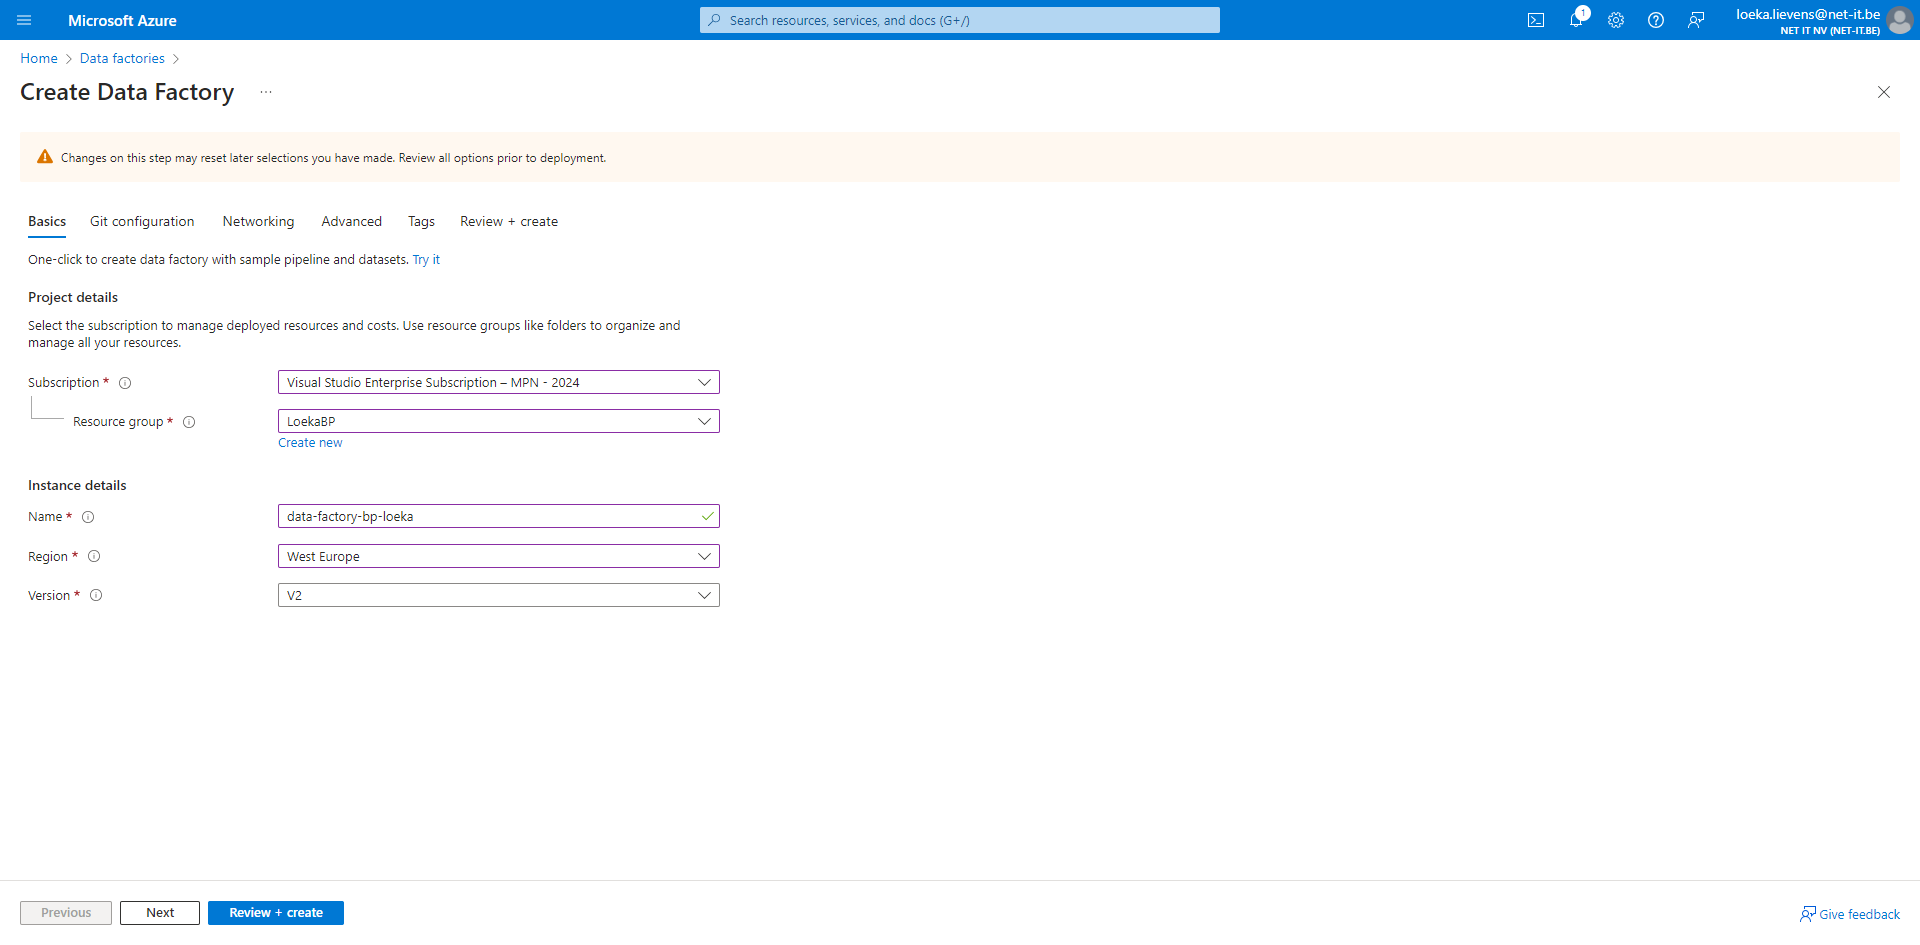
\includegraphics[width=1\textwidth]{./graphics/adf/initial_1.png}
%\end{center}
%
%Selecteer een gewenste subsscription en resource group. Er kan gekozen worden voor een resource group die er al bestaat of om een nieuwe aan te maken. Hier na kan er een naam en gewenste regio gekozen worden. De version laten we staan op V2.
%
%\begin{center}
%    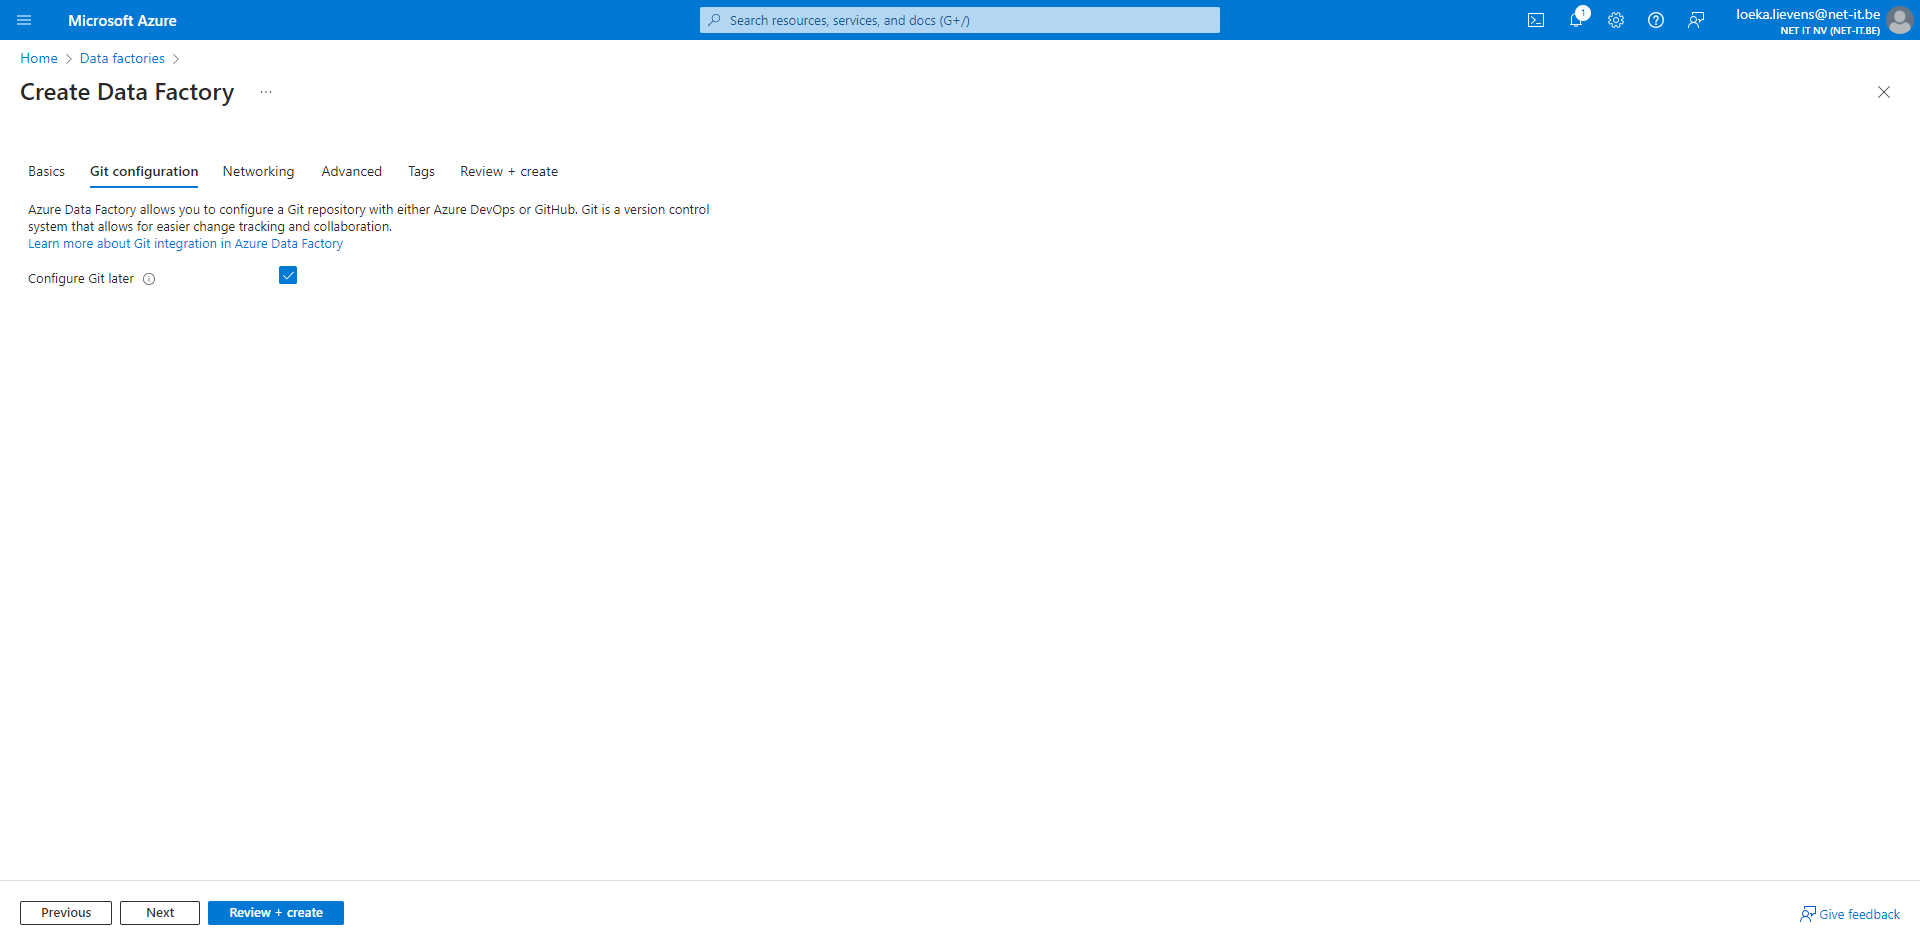
\includegraphics[width=1\textwidth]{./graphics/adf/initial_2.png}
%\end{center}
%
%Door bij de vorige stap op next te klikken kunnen we er voor kiezen om een Git configuratie te gaan toevoegen. Dit zullen we pas later gaan doen. Klik nu op `Review + create` om de data factory aan te maken.
%
%\begin{center}
%    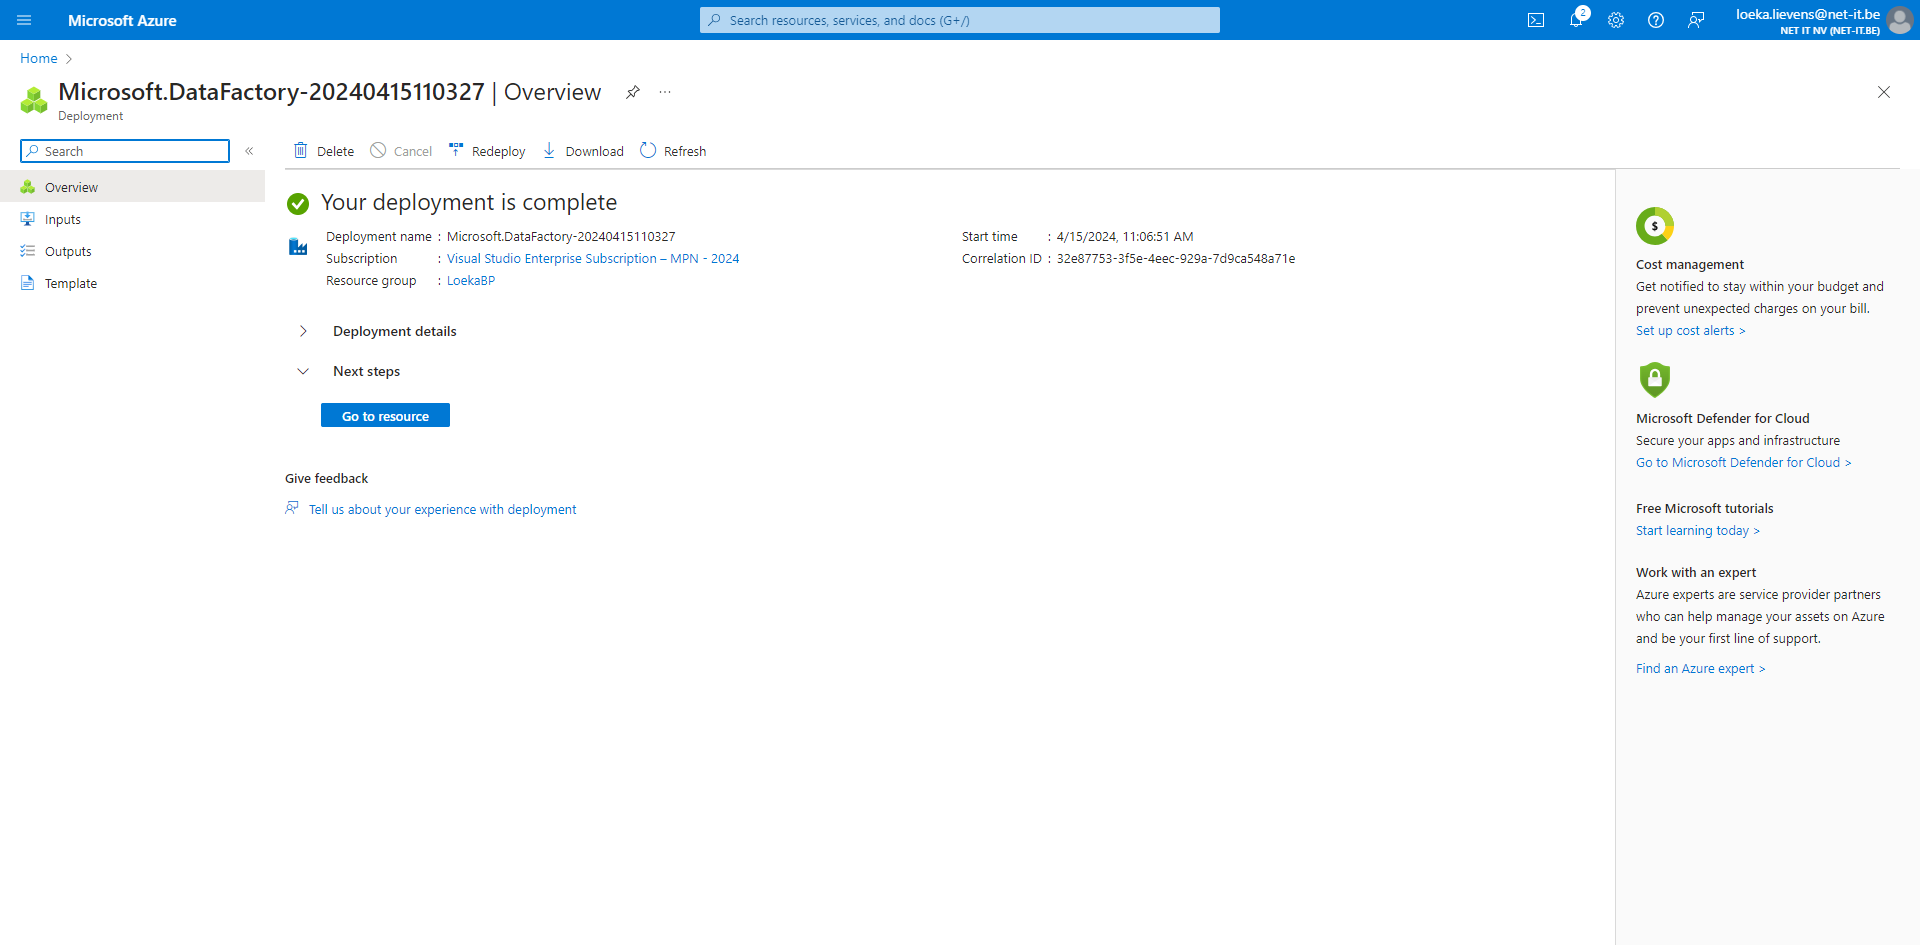
\includegraphics[width=1\textwidth]{./graphics/adf/deployment_complete.png}
%\end{center}
%
%Wanneer onze deployment complete is kunnen we naar onze resource gaan door op `Go to resource` te klikken.
%
%\begin{center}
%    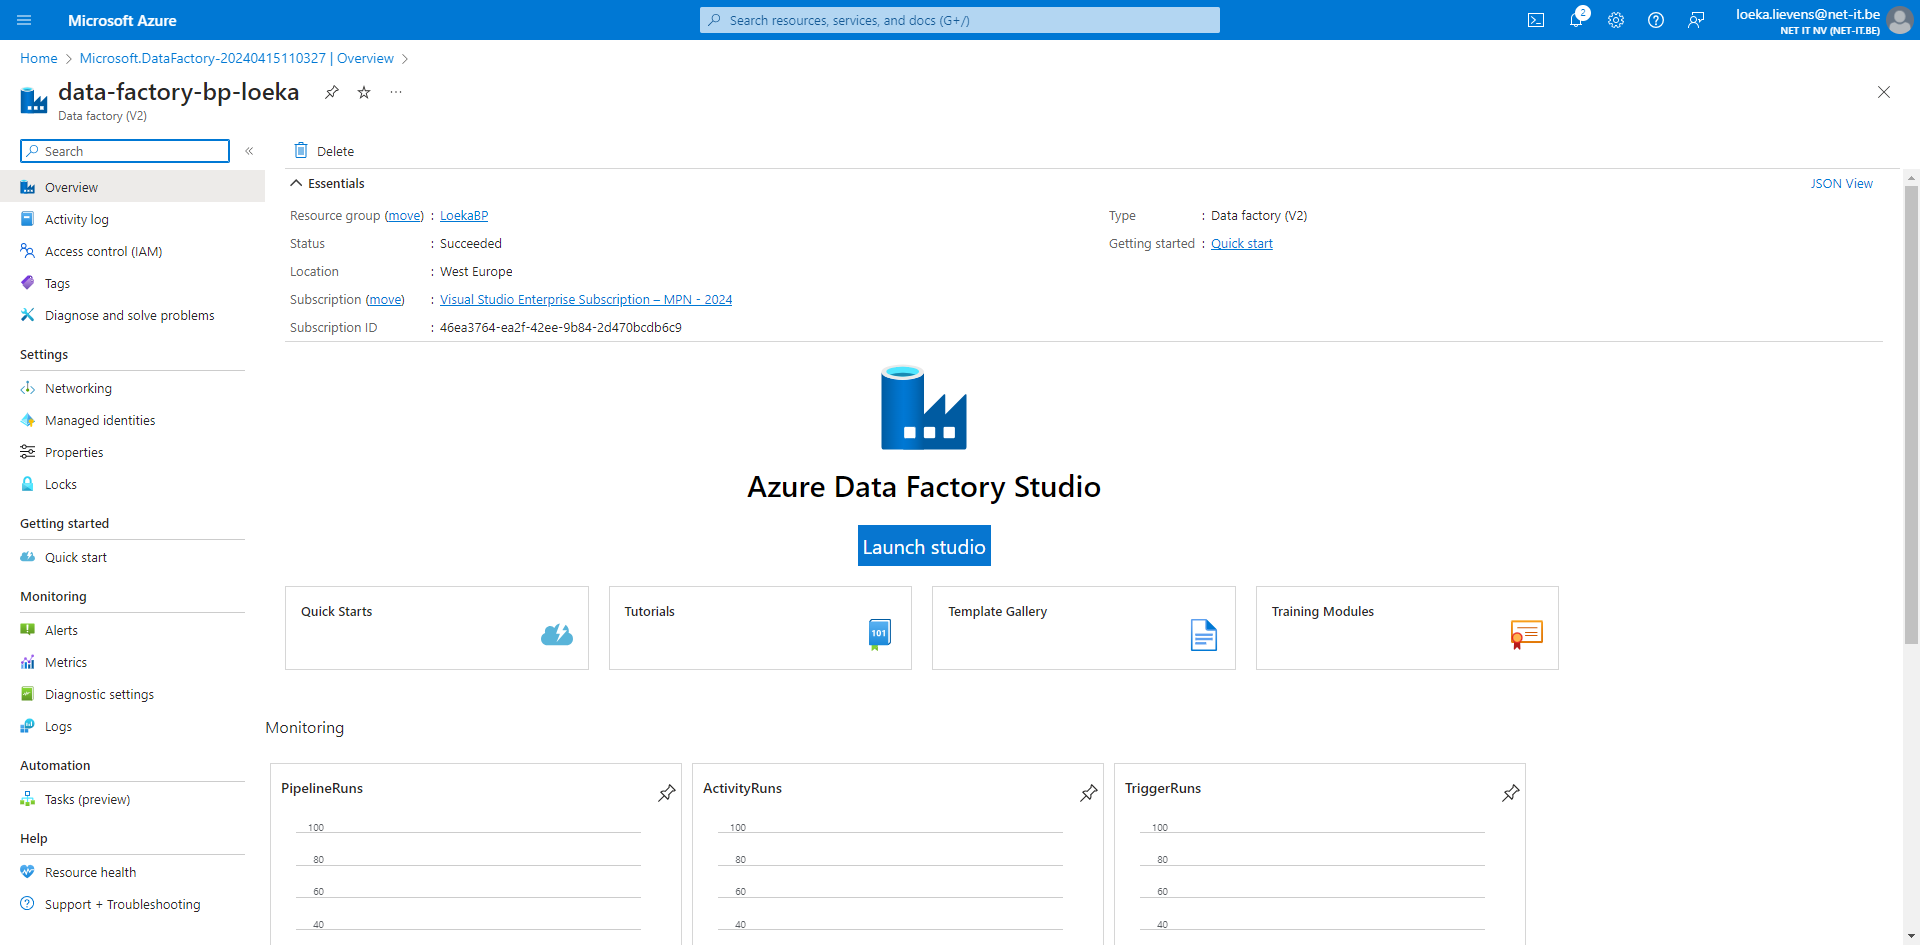
\includegraphics[width=1\textwidth]{./graphics/adf/launch_adf.png}
%\end{center}
%
%Klik nu op `Launch studio` om naar Azure Data Factory Studio te gaan.
%
%\subsubsection{Koppeling met Git}
%
%\begin{center}
%    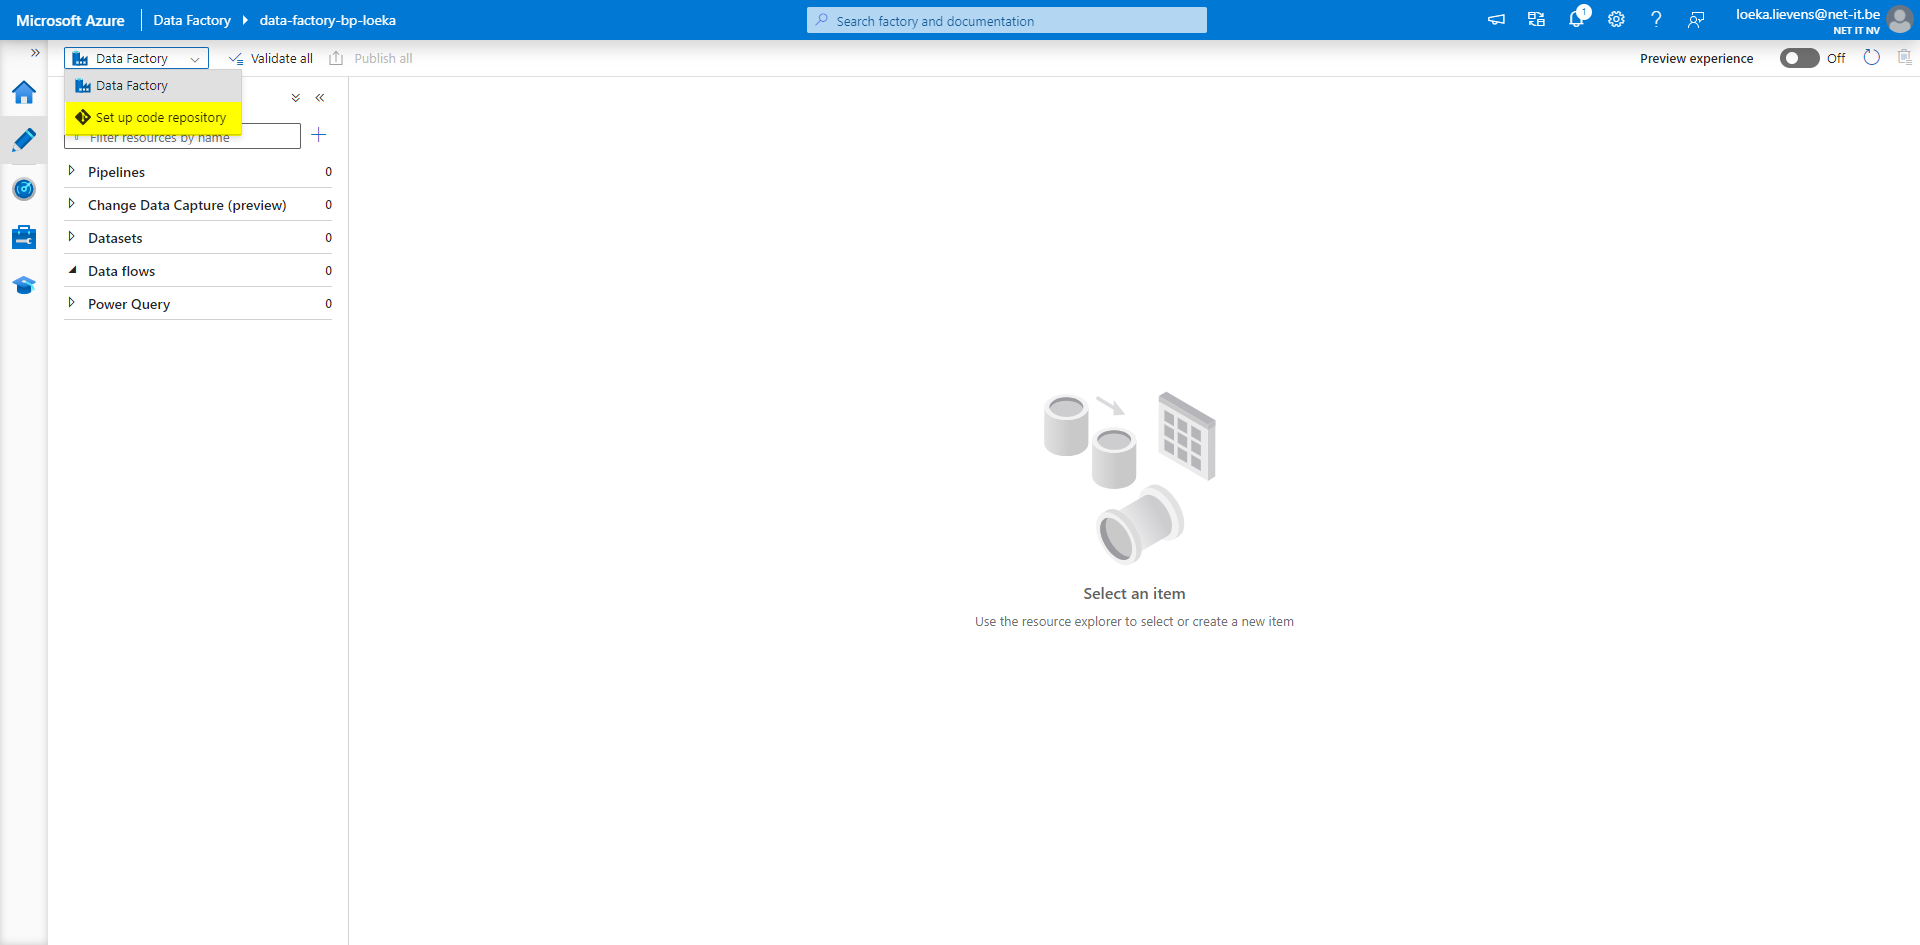
\includegraphics[width=1\textwidth]{./graphics/adf/setup_repository.png}
%\end{center}
%
%Voor we onze ETL gaan implementeren zullen we eerst onze data factory koppelen met Git.
%
%\begin{center}
%    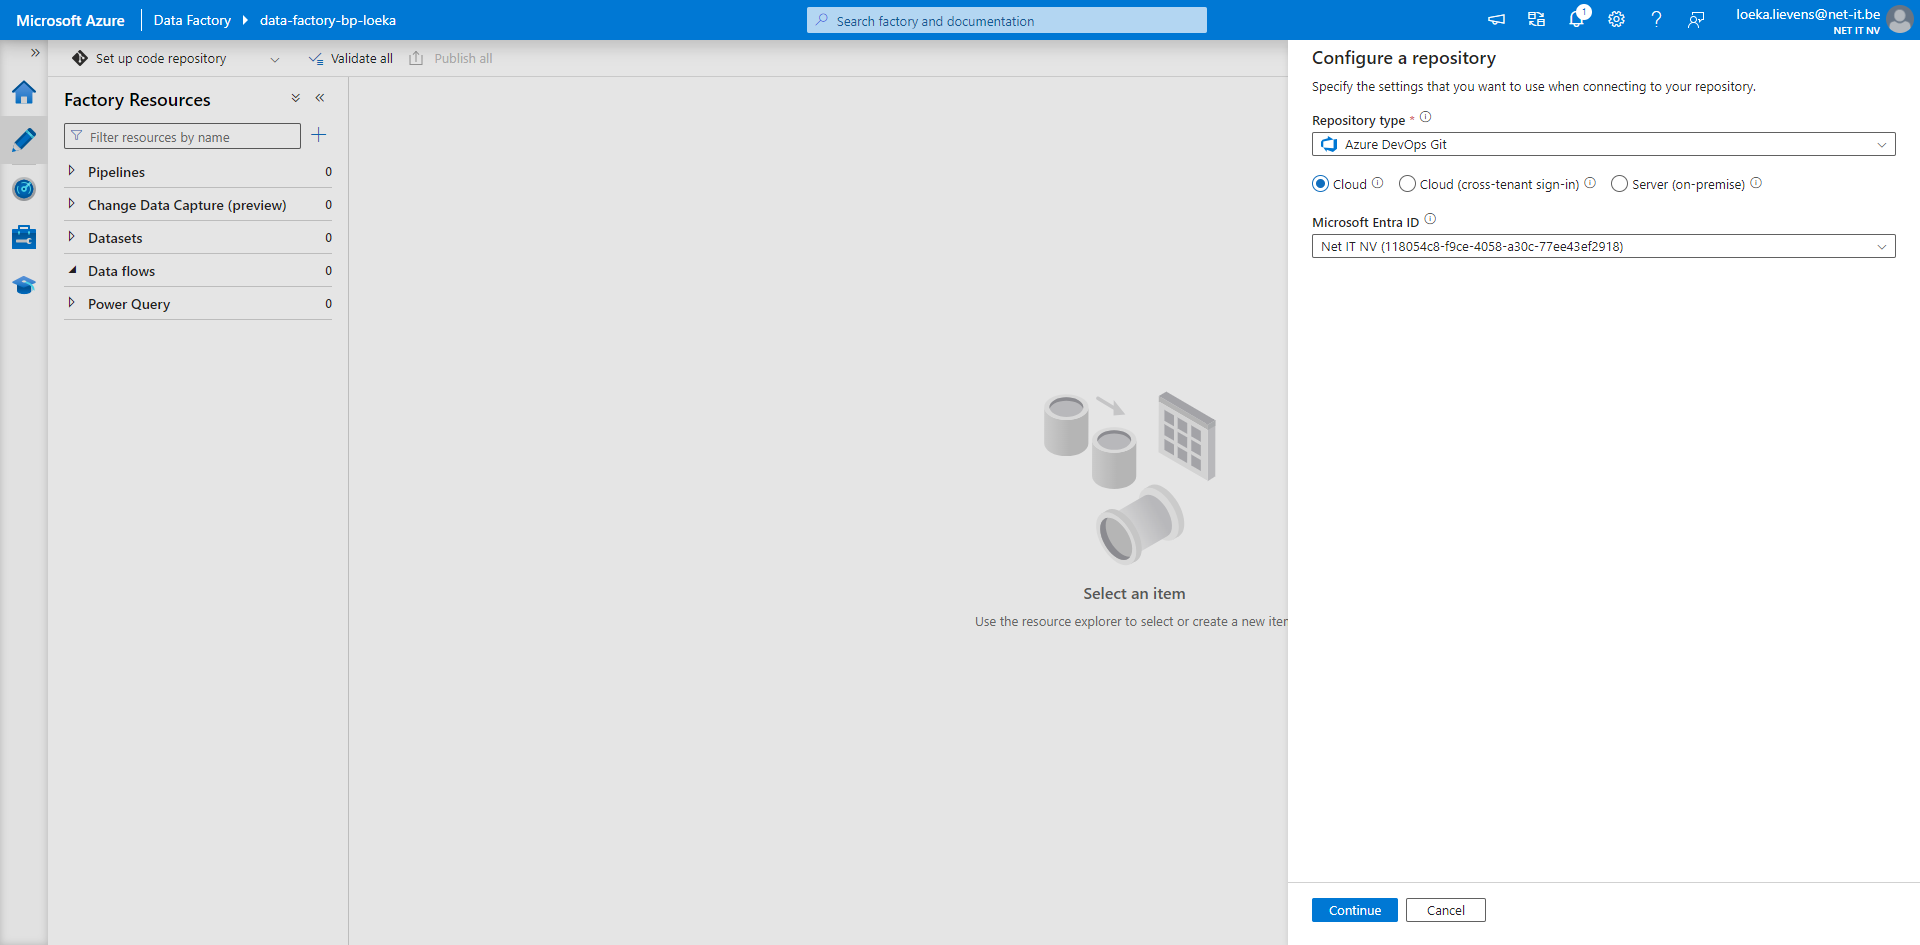
\includegraphics[width=1\textwidth]{./graphics/adf/setup_repository_2.png}
%\end{center}
%
%\begin{center}
%    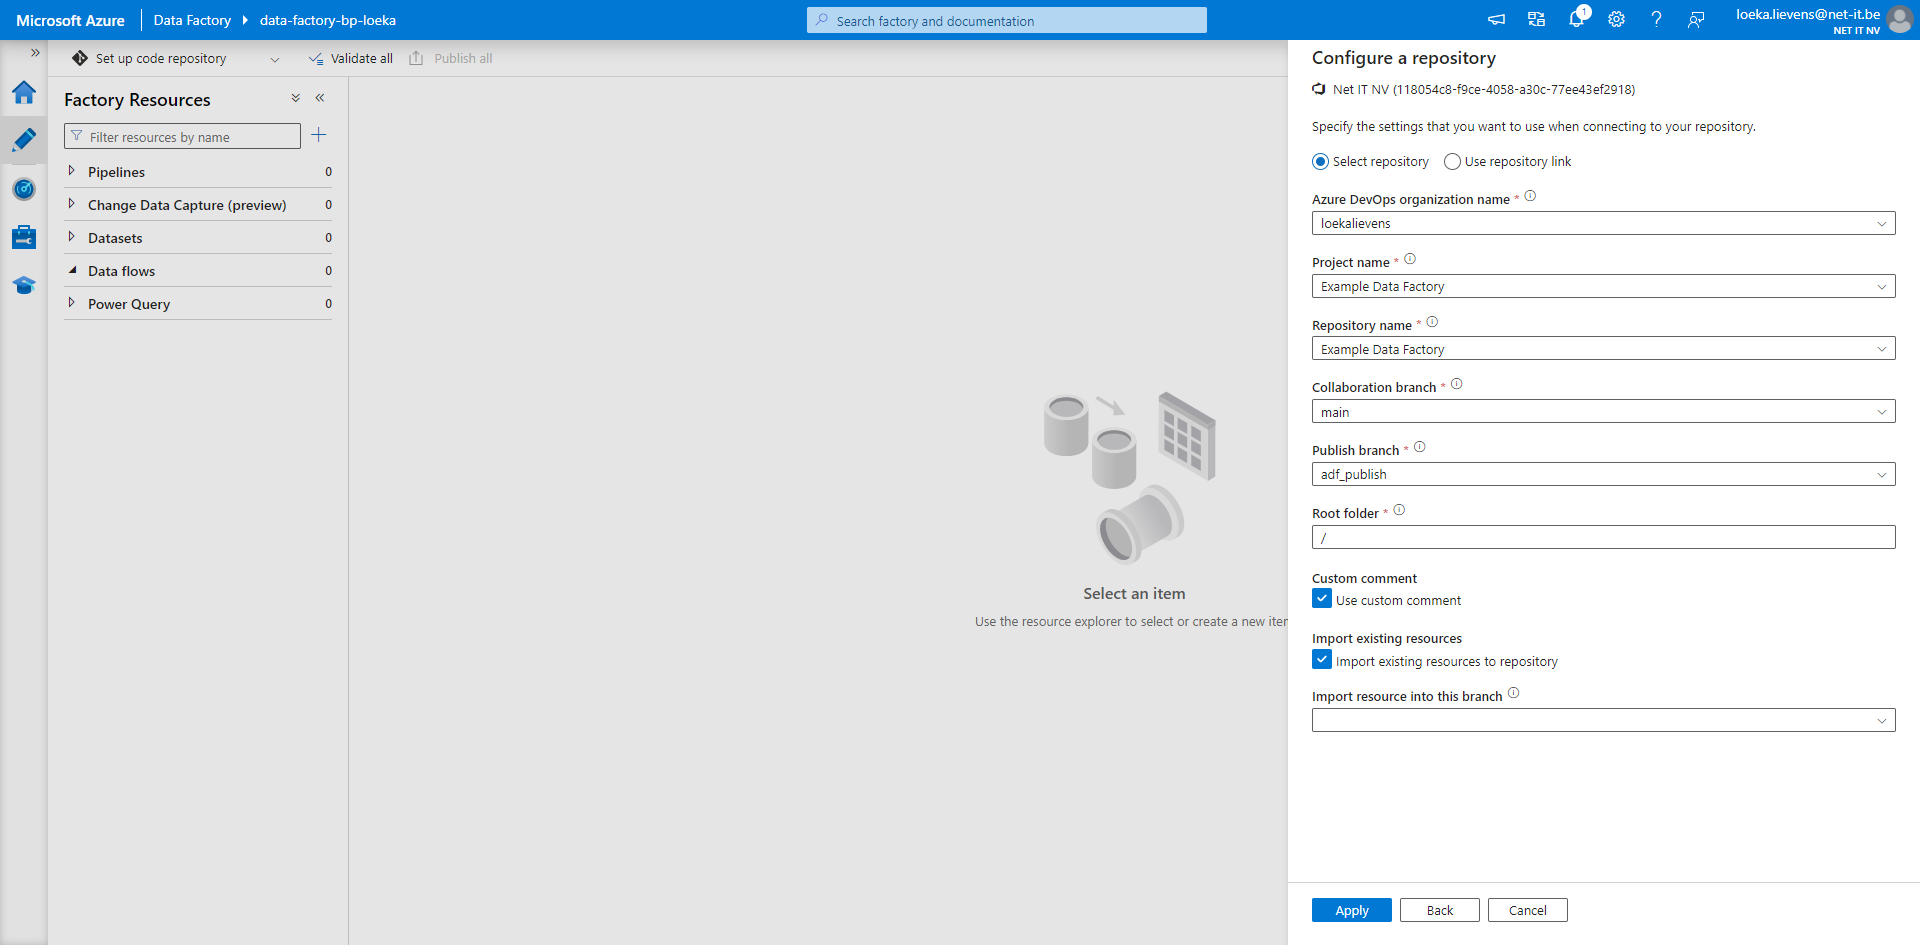
\includegraphics[width=1\textwidth]{./graphics/adf/setup_repository_3.png}
%\end{center}
%
%Binnen Net IT wordt er gewerkt met Azure DevOps Git.
%
%\subsubsection{Het toevoegen van een source}
%
%Telkens wanneer we een source tabel zullen gaan toevoegen zal dit op dezelfde manier gebeuren.
%
%\begin{center}
%    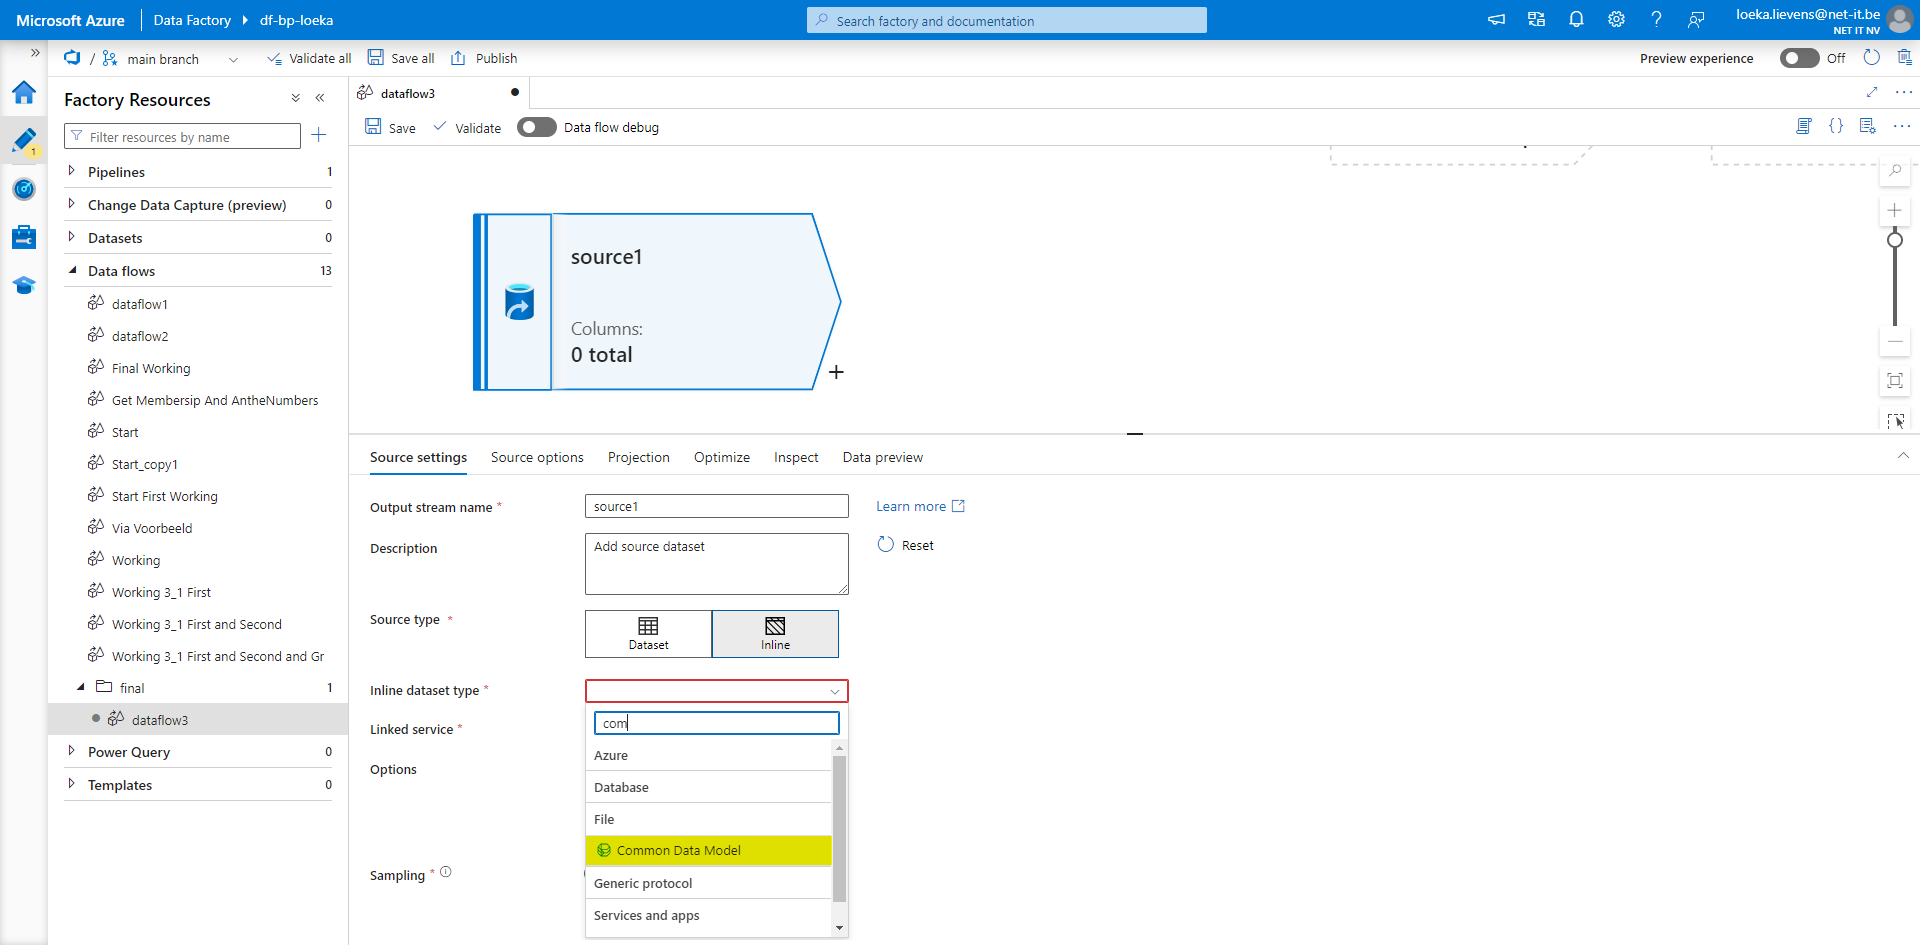
\includegraphics[width=1\textwidth]{./graphics/adf/source_table_1.png}
%\end{center}
%
%Als source type zal er steeds gekozen worden voor inline. Dit doordat we slechts één enkele dataflow zullen gaan aanmaken en geen gedeelde datasets nodig hebben. Als type voor de linked service kiezen we voor Common Data Model.
%
%\begin{center}
%    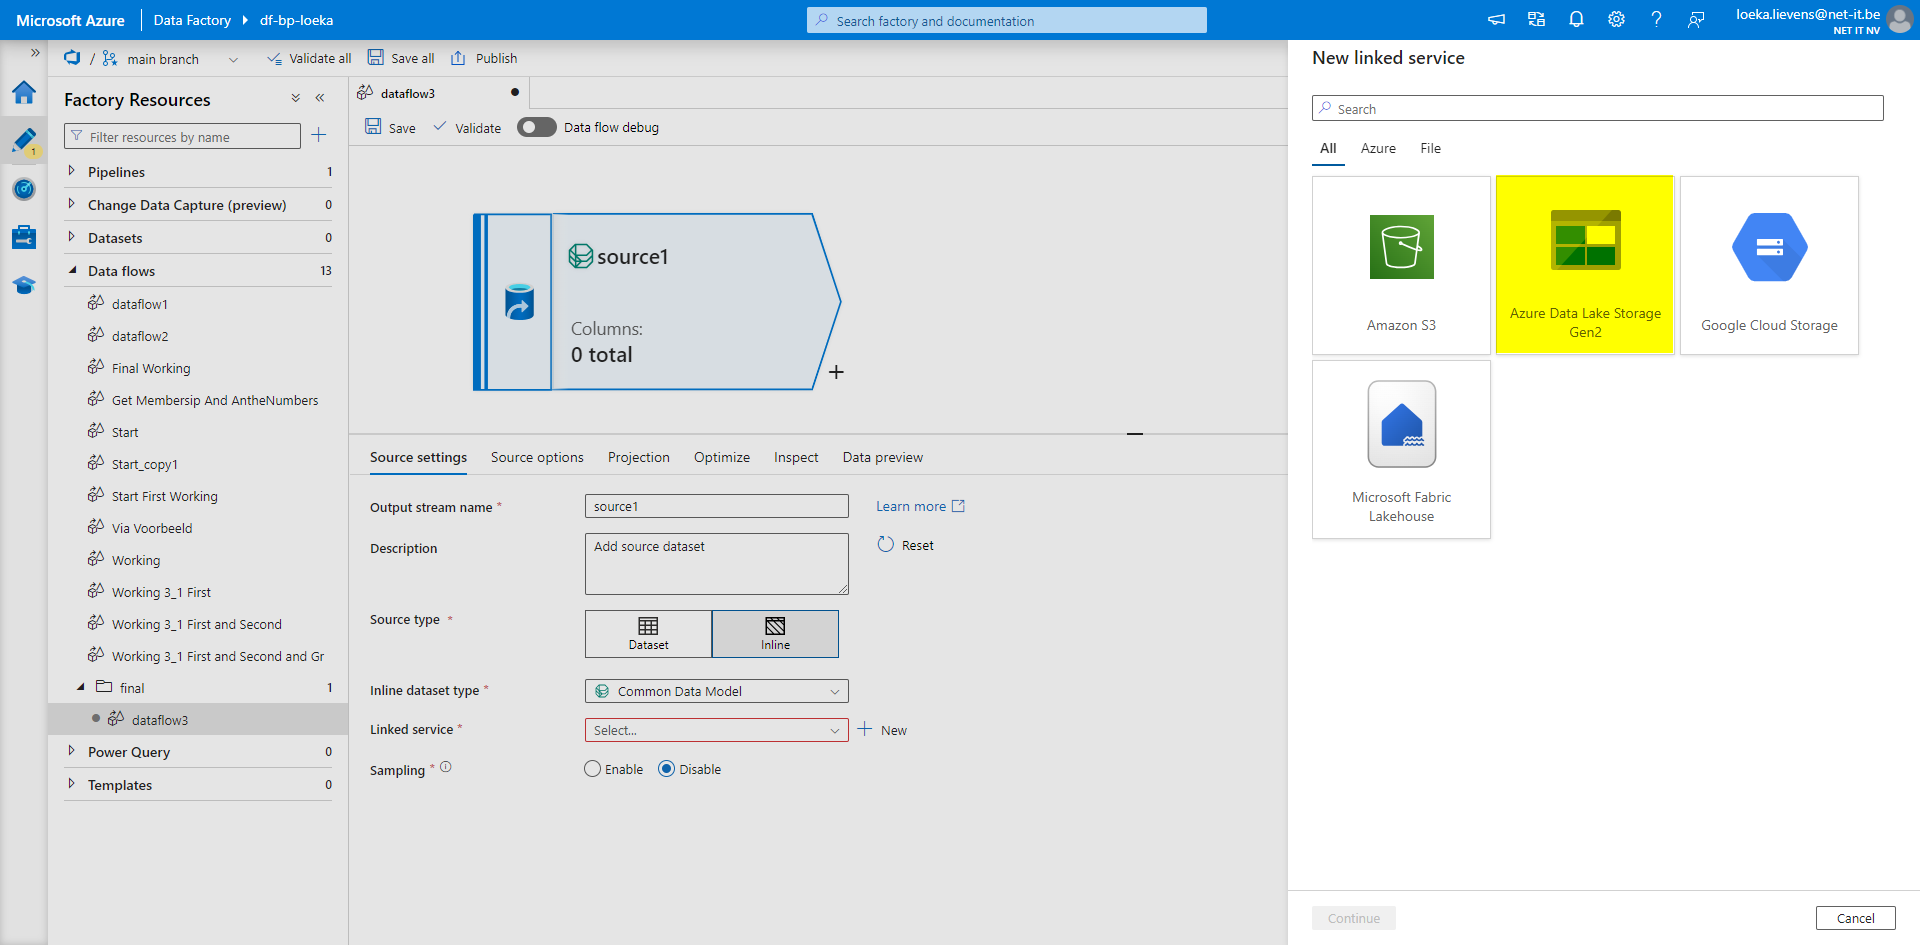
\includegraphics[width=1\textwidth]{./graphics/adf/source_table_2.png}
%\end{center}
%
%Er zal éénmalig een Linked Service aangemaakt moeten worden. Hierbij kiezen we voor Azure Data Lake Storage Gen2.
%
%\begin{center}
%    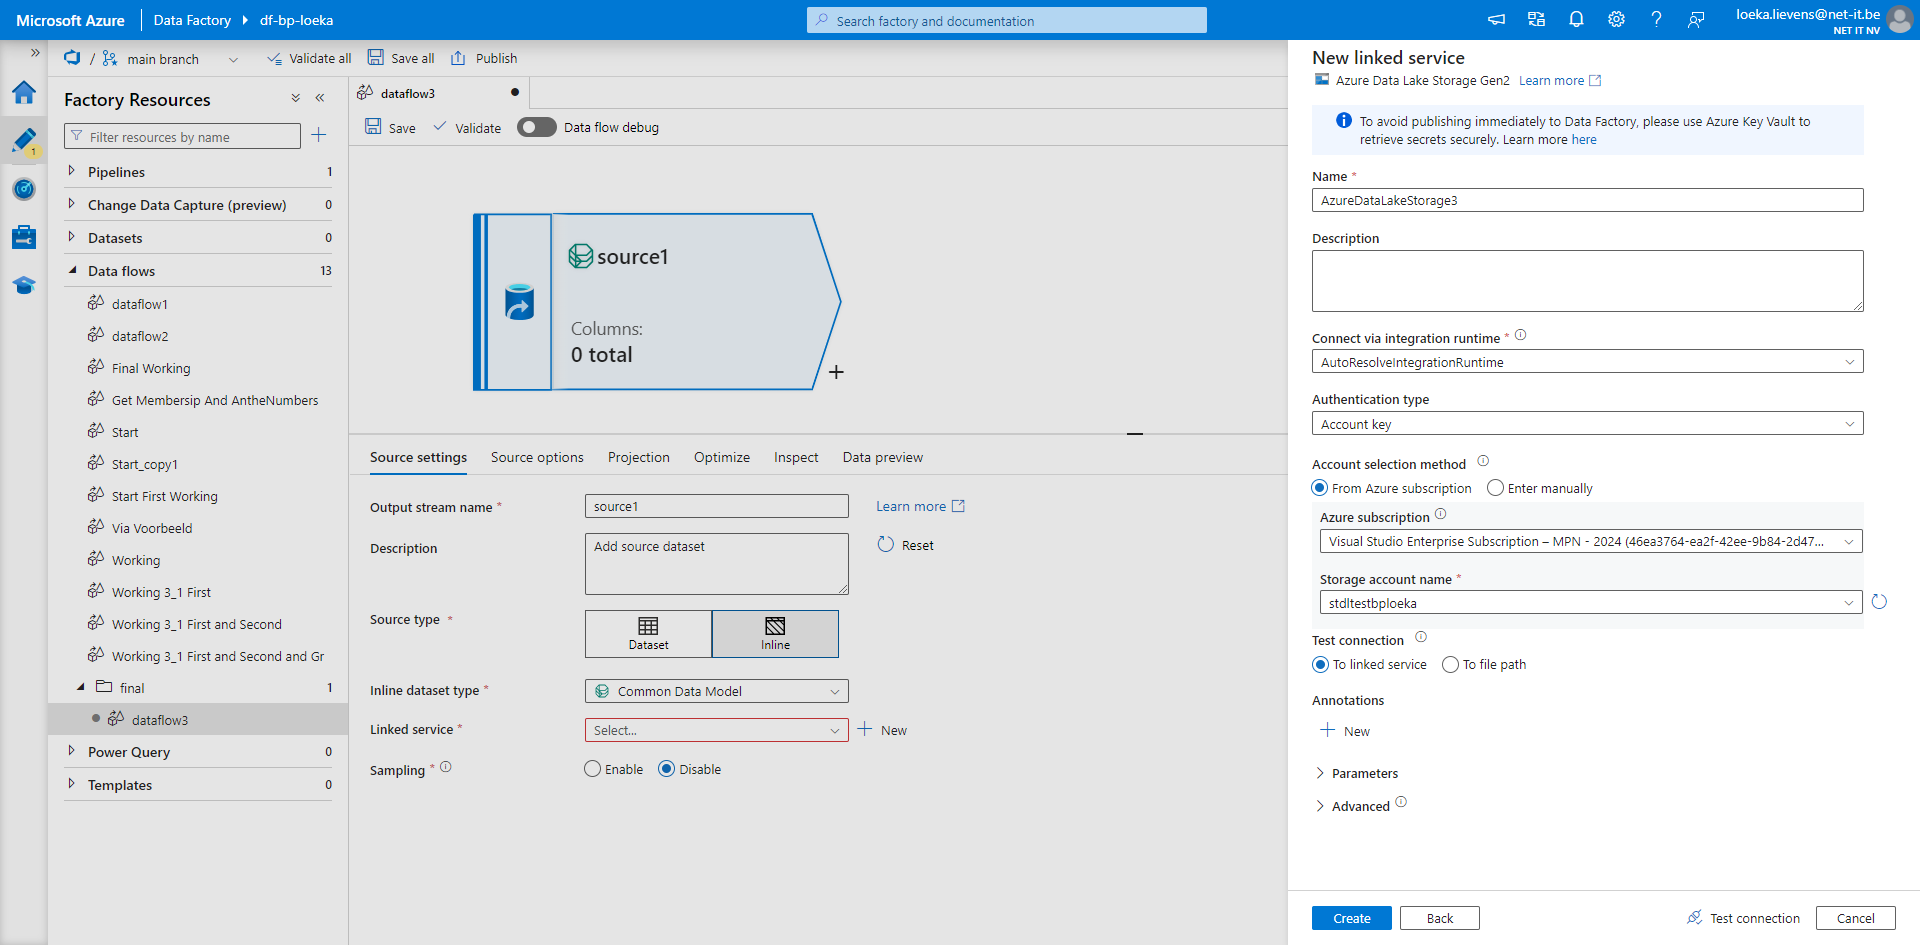
\includegraphics[width=1\textwidth]{./graphics/adf/source_table_3.png}
%\end{center}
%
%We kunnen makkelijk gaan koppelen met de juiste data lake door een Azure Subscription en Storage account name aan te duiden. Door op `Test connection` te klikken kunnen we kijken of de connectie met data lake is gelukt. Door op `Create` te klikken hebben we nu een Linked Service die steeds bij elke Source gebruikt kan worden.
%
%\begin{center}
%    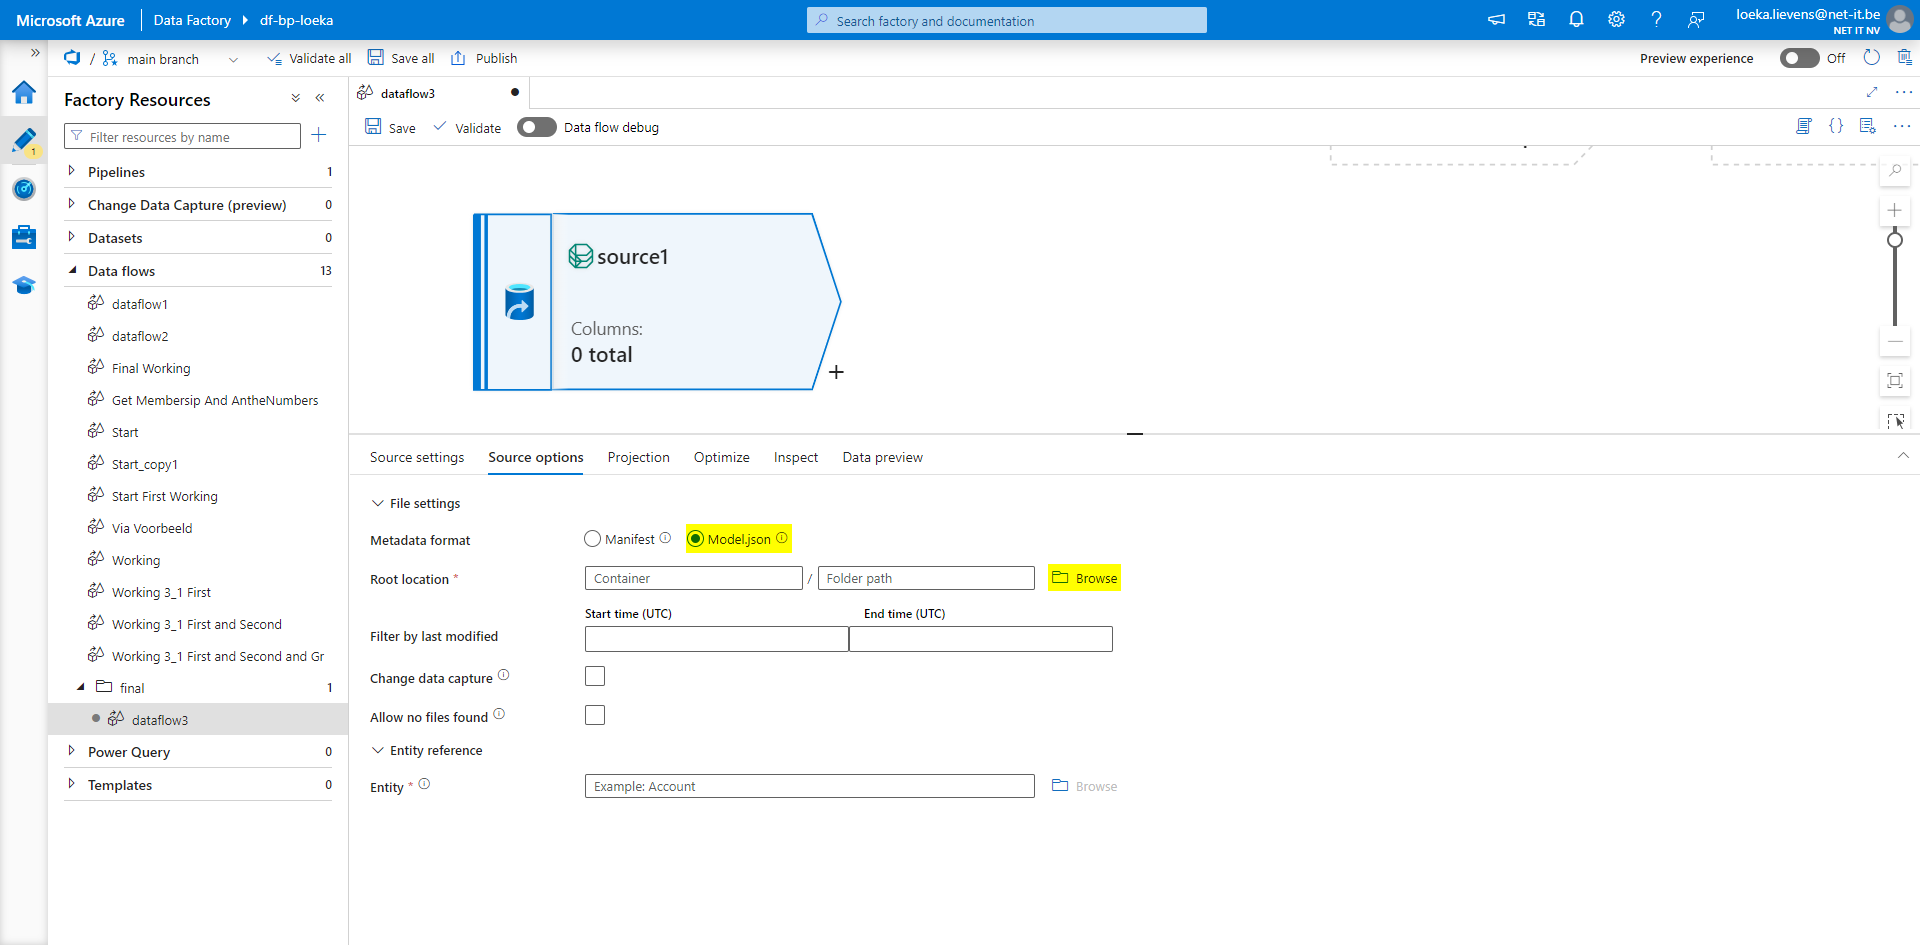
\includegraphics[width=1\textwidth]{./graphics/adf/source_table_4.png}
%\end{center}
%
%Door naar `Source options` te gaan kunnen we `Model.json` gaan aanduiden. Door op `Browse` te klikken kunnen we aanduiden waar het Model.json bestand te vinden is in data lake.
%
%\begin{center}
%    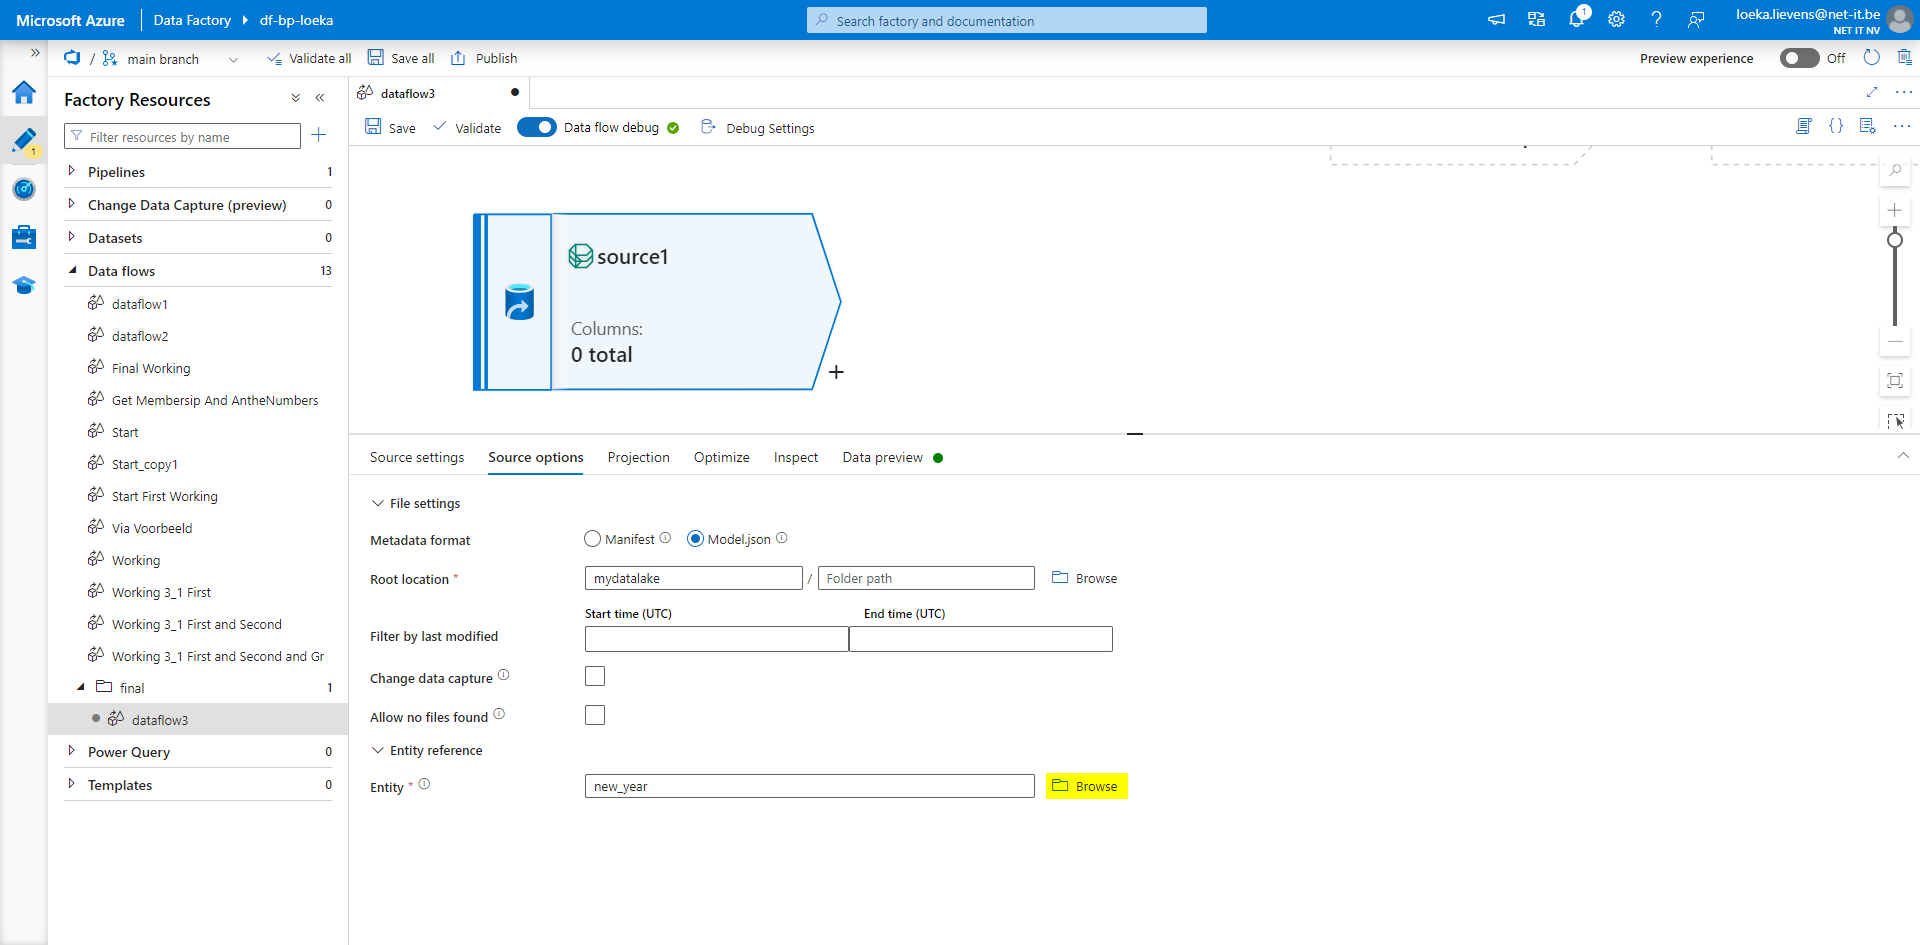
\includegraphics[width=1\textwidth]{./graphics/adf/source_table_5.png}
%\end{center}
%
%Naast `Entity` kunnen we nu op `Browse` klikken om de gewenste entity te gaan importeren. Let op: hier voor zal Data flow debug aan moeten staan.
%
%\begin{center}
%    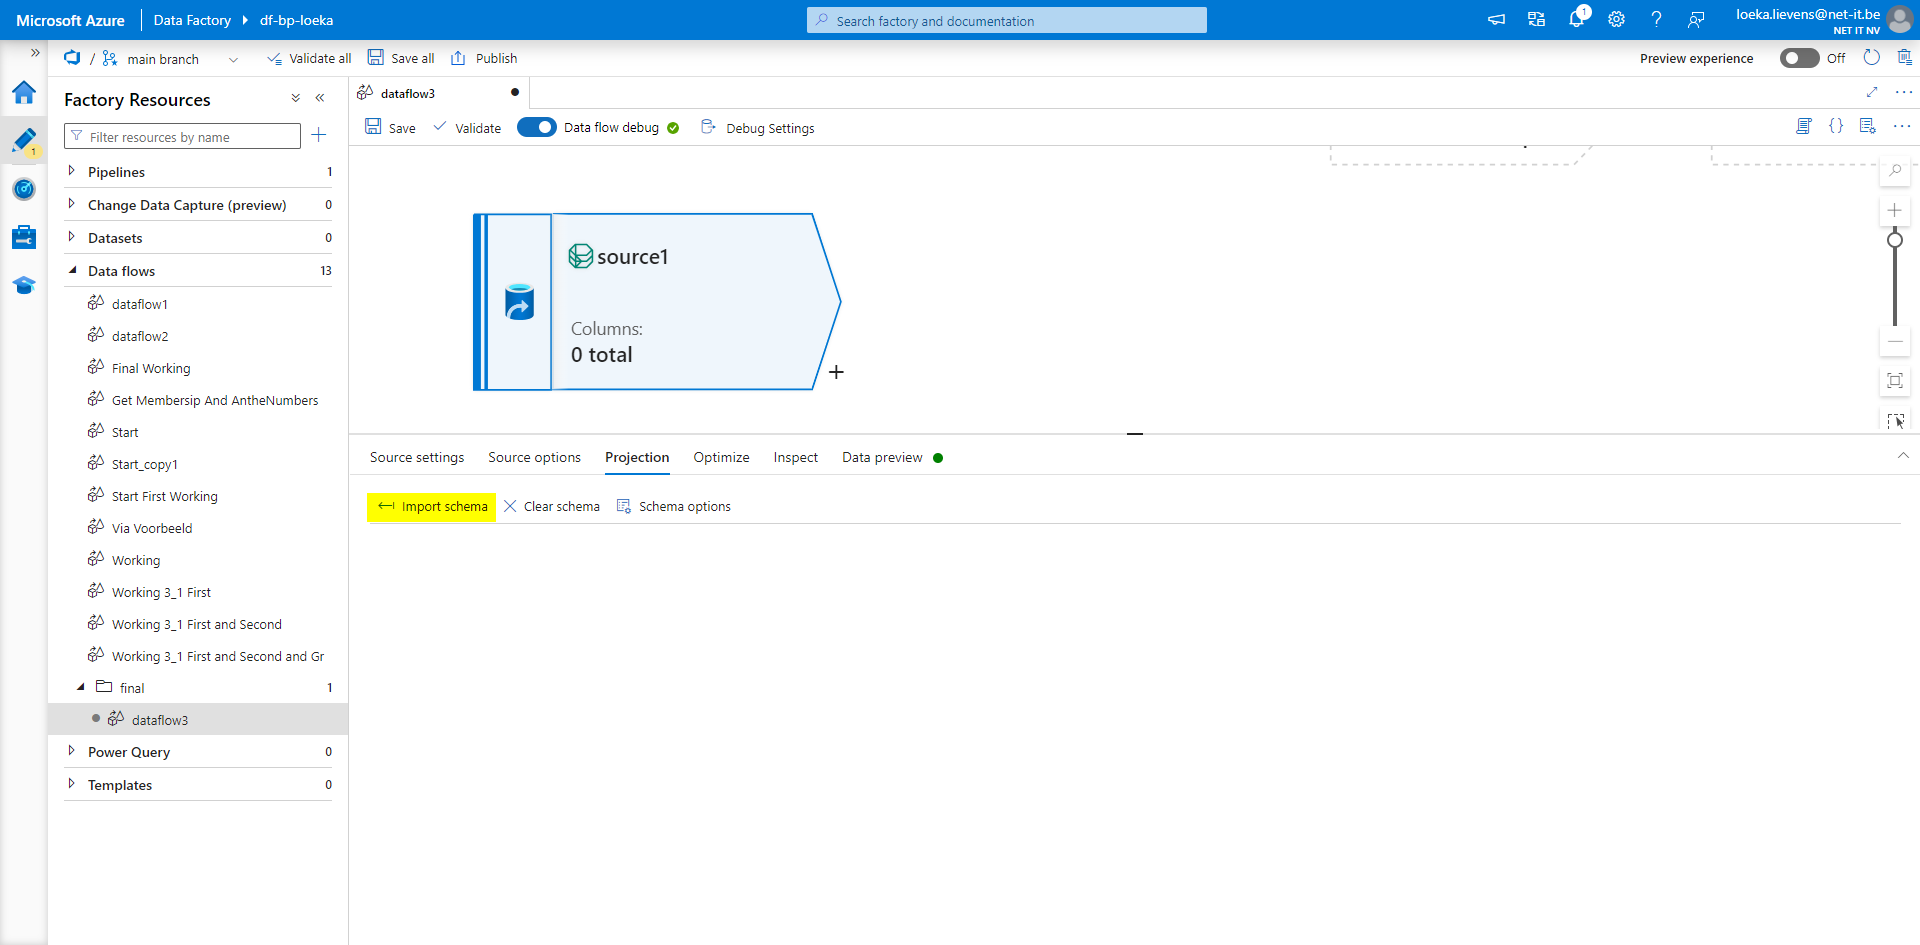
\includegraphics[width=1\textwidth]{./graphics/adf/source_table_6.png}
%\end{center}
%
%Door naar `Projection` te gaan kunnen we nu op `Import schema` klikken.
%
%\begin{center}
%    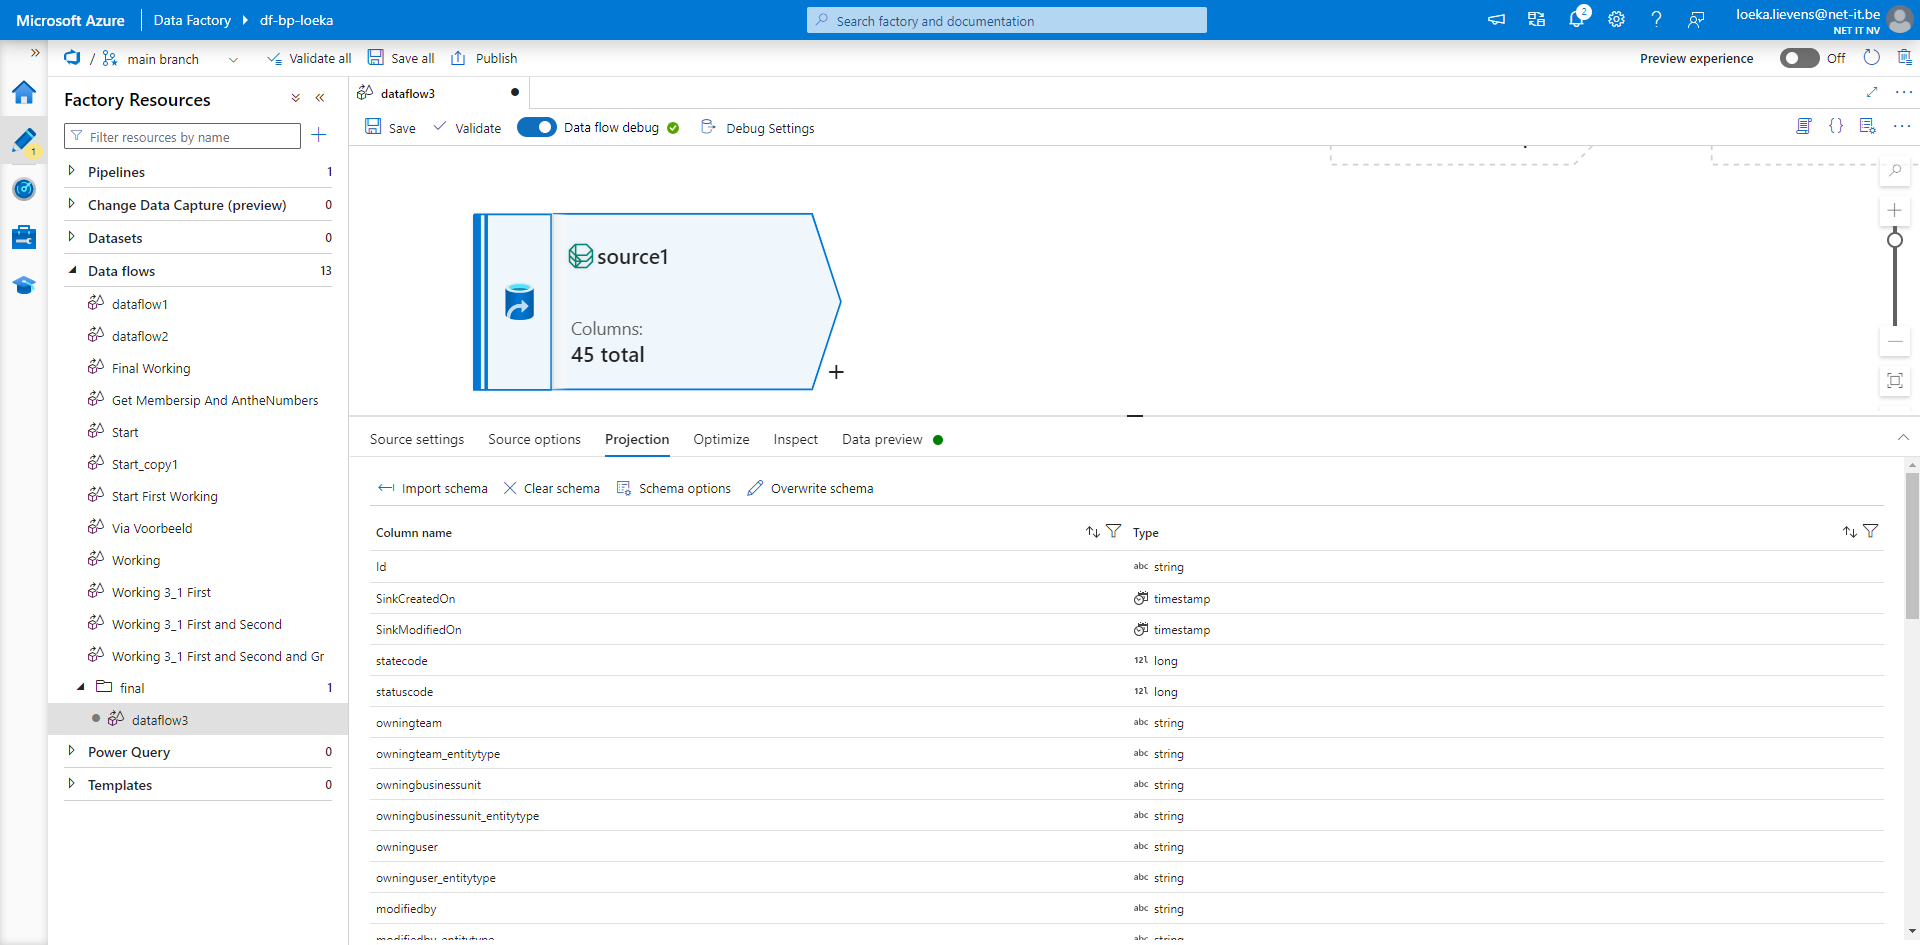
\includegraphics[width=1\textwidth]{./graphics/adf/source_table_7.png}
%\end{center}
%
%De foto hierboven toont een voorbeeld van een geïmporteerd schema.
%
%\begin{center}
%    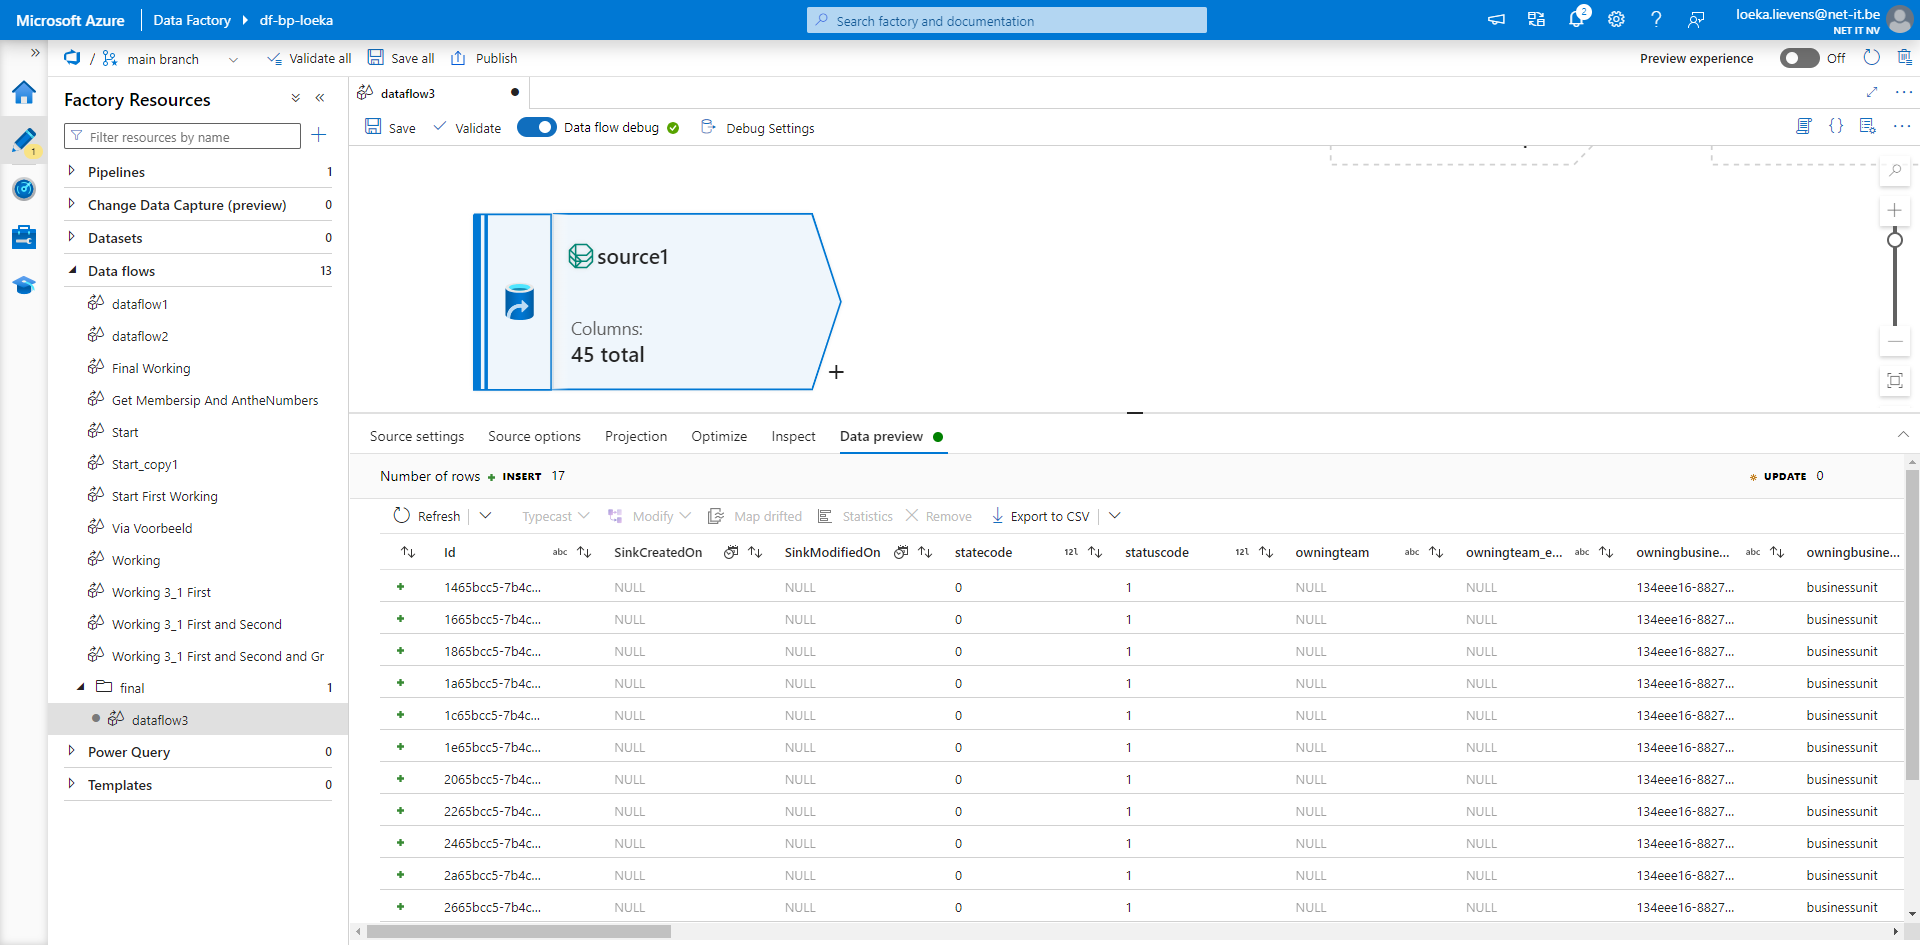
\includegraphics[width=1\textwidth]{./graphics/adf/source_table_8.png}
%\end{center}
%
%Wanneer we naar `Data preview` gaan kunnen we een preview zien van de data uit de gekozen tabel.
%
%\subsubsection{Implementatie ETL}
%
%\begin{center}
%    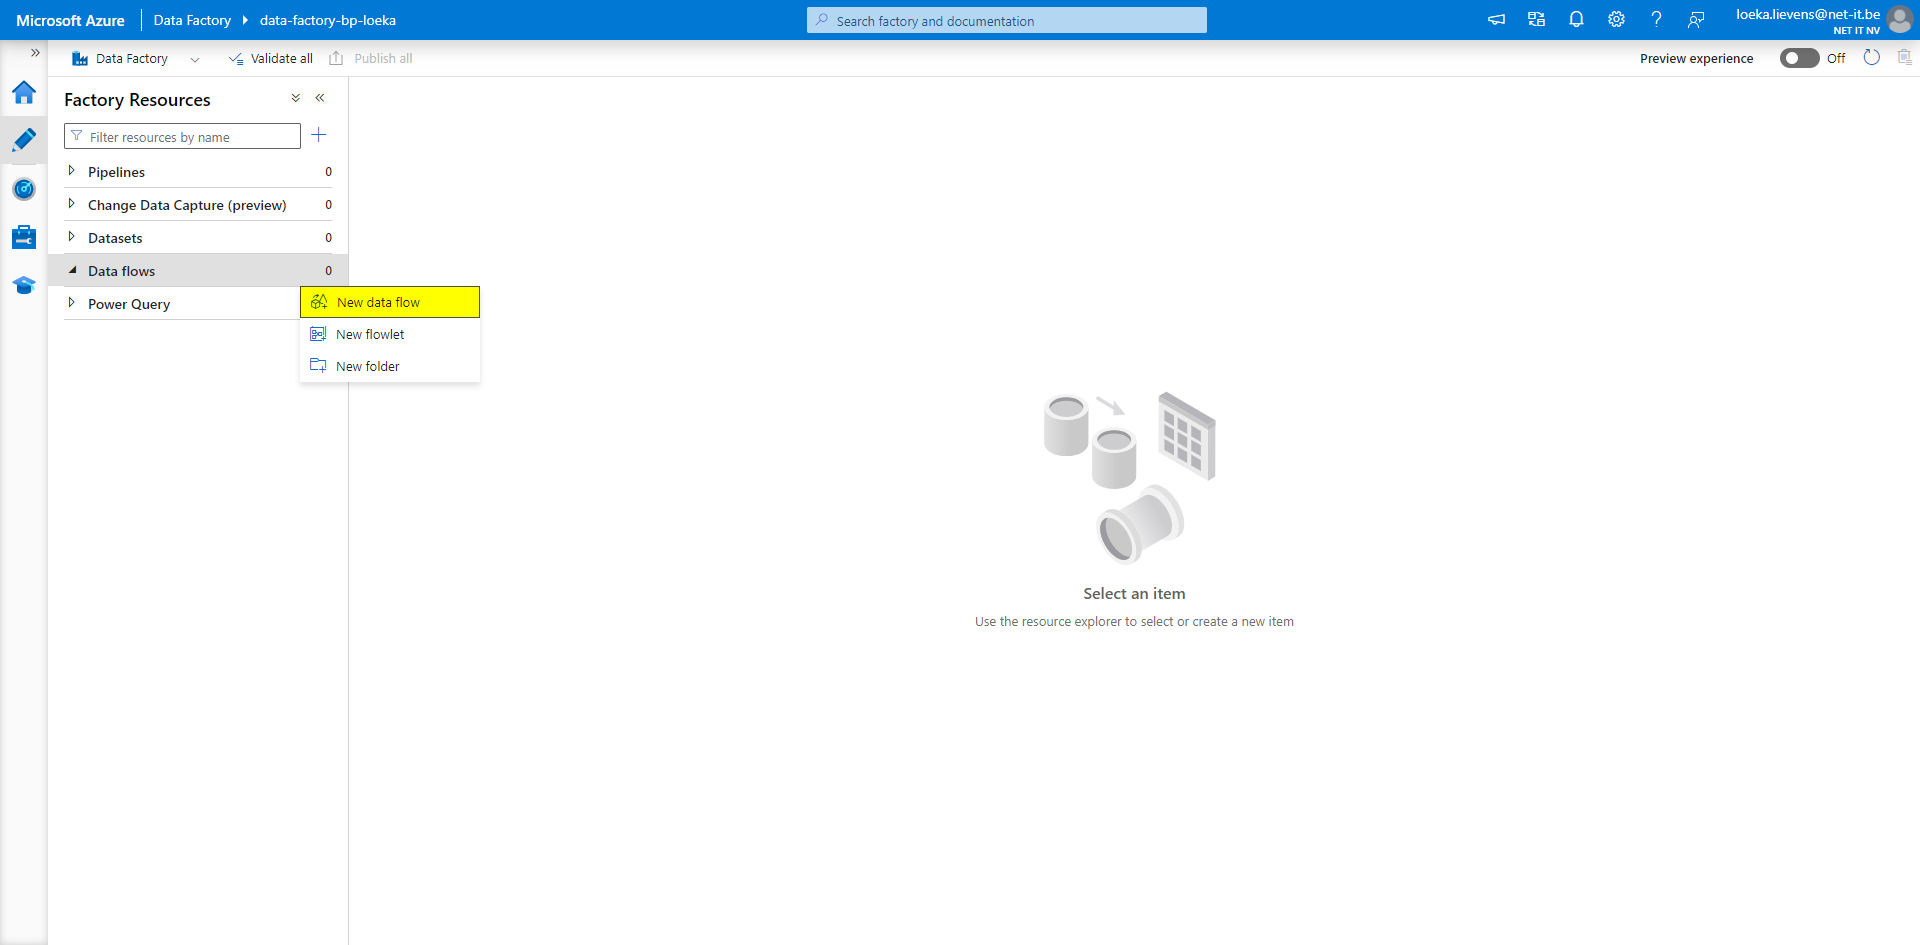
\includegraphics[width=1\textwidth]{./graphics/adf/dataflow.png}
%\end{center}
%
%Voor het implementeren van onze ETL gaan we een nieuwe dataflow gaan aanmaken.
%
%\paragraph{\texttt{Tabel new\_person}}
%
%\begin{center}
%    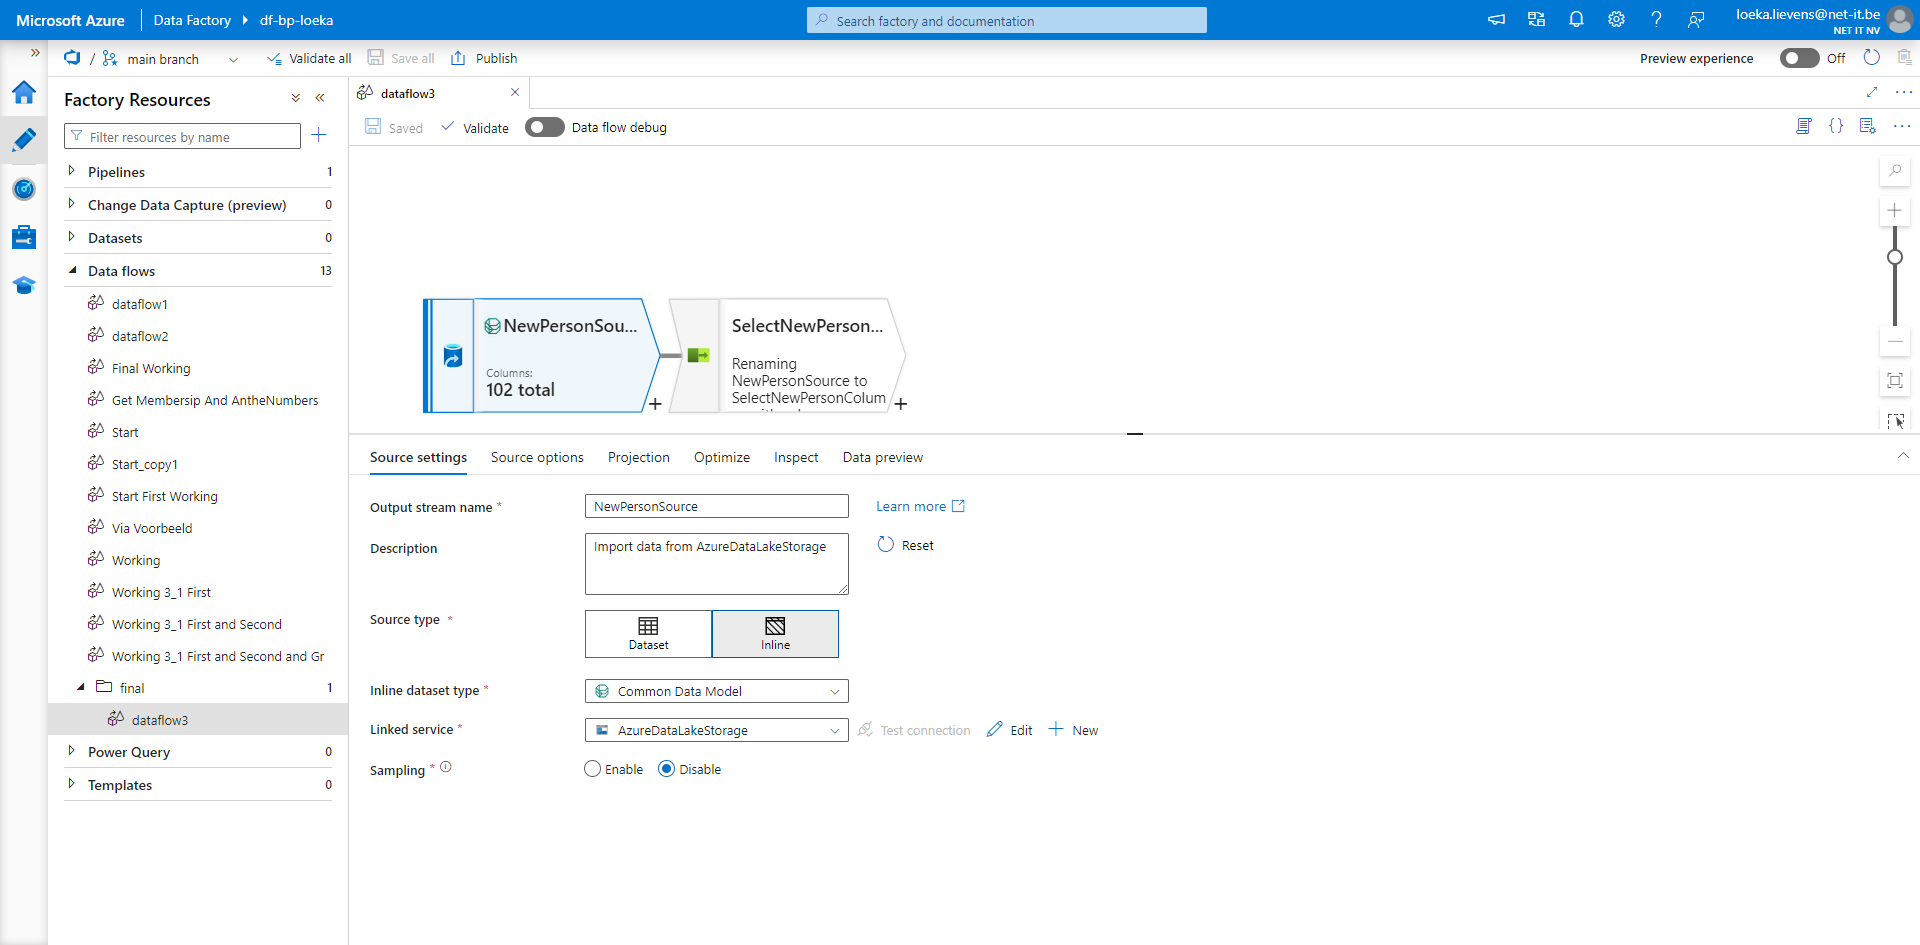
\includegraphics[width=1\textwidth]{./graphics/adf/new_person_source.png}
%\end{center}
%
%\texttt{Er wordt een source toegevoegd voor de tabel new\_person.}
%
%\begin{center}
%    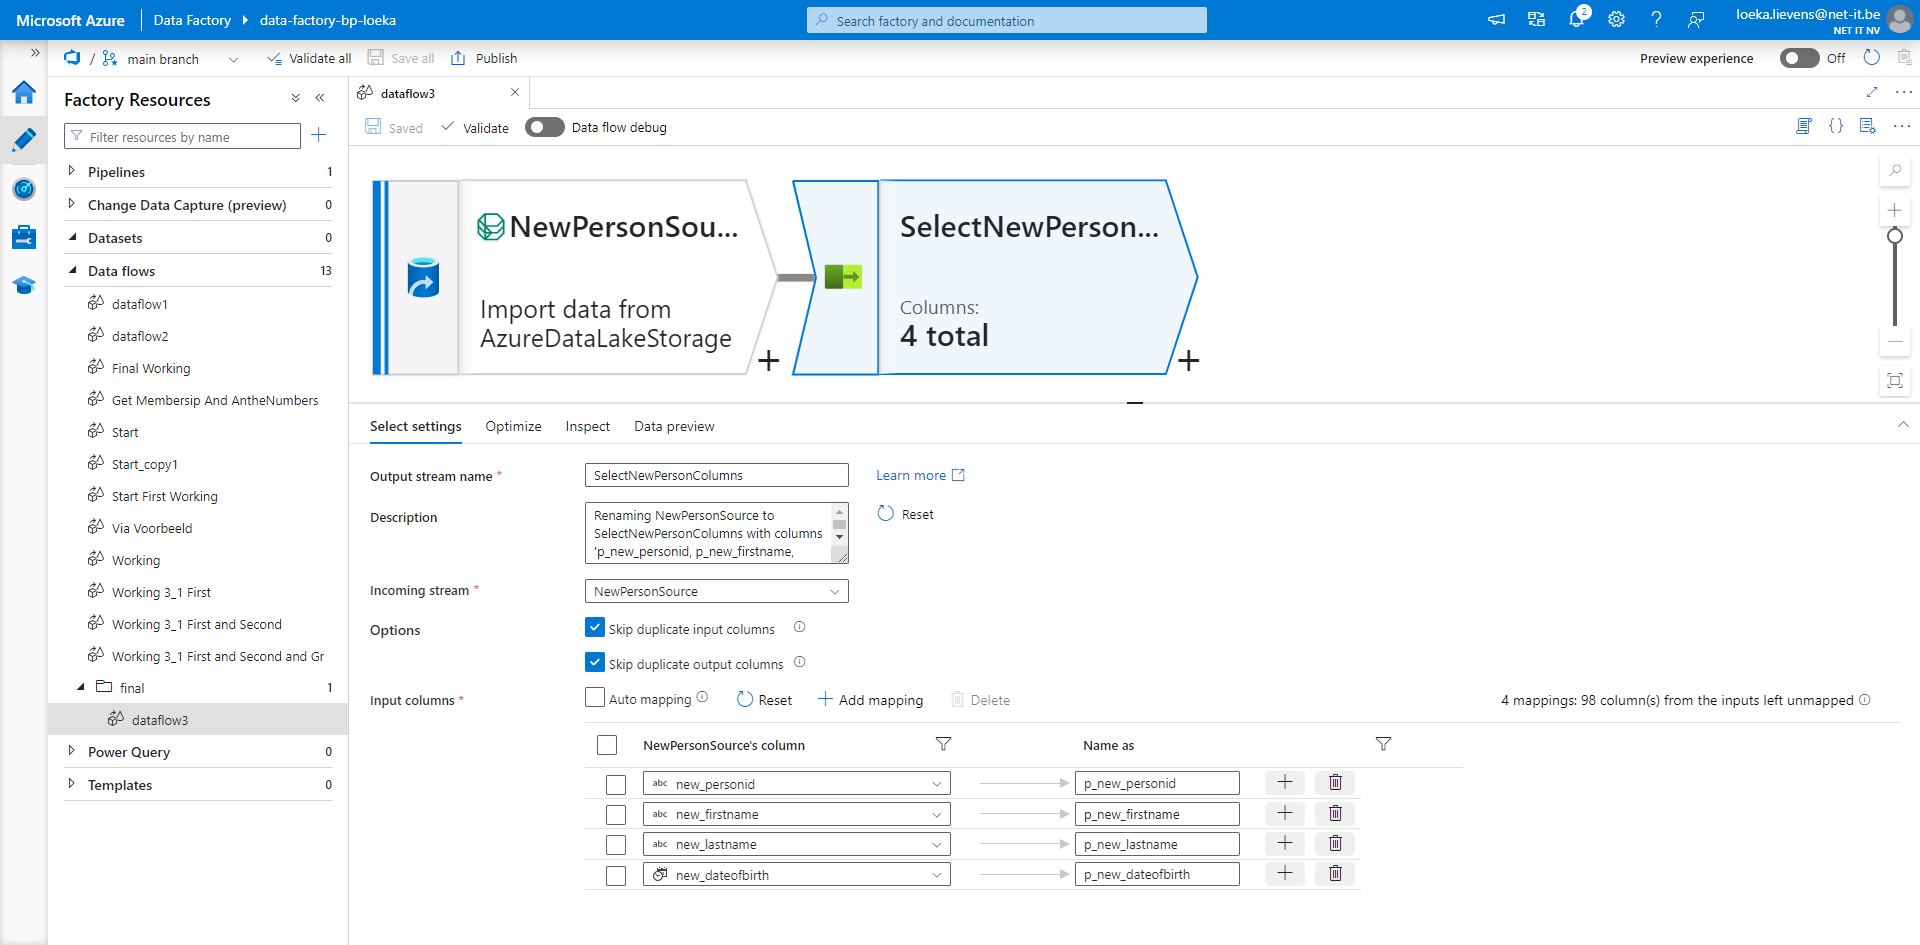
\includegraphics[width=1\textwidth]{./graphics/adf/new_person_select.png}
%\end{center}
%
%\texttt{De nodige kolommen worden geselecteerd en hernoemt met de prefix `p\_`.}
%
%\paragraph{\texttt{Tabel new\_bankaccount}}
%
%\begin{center}
%    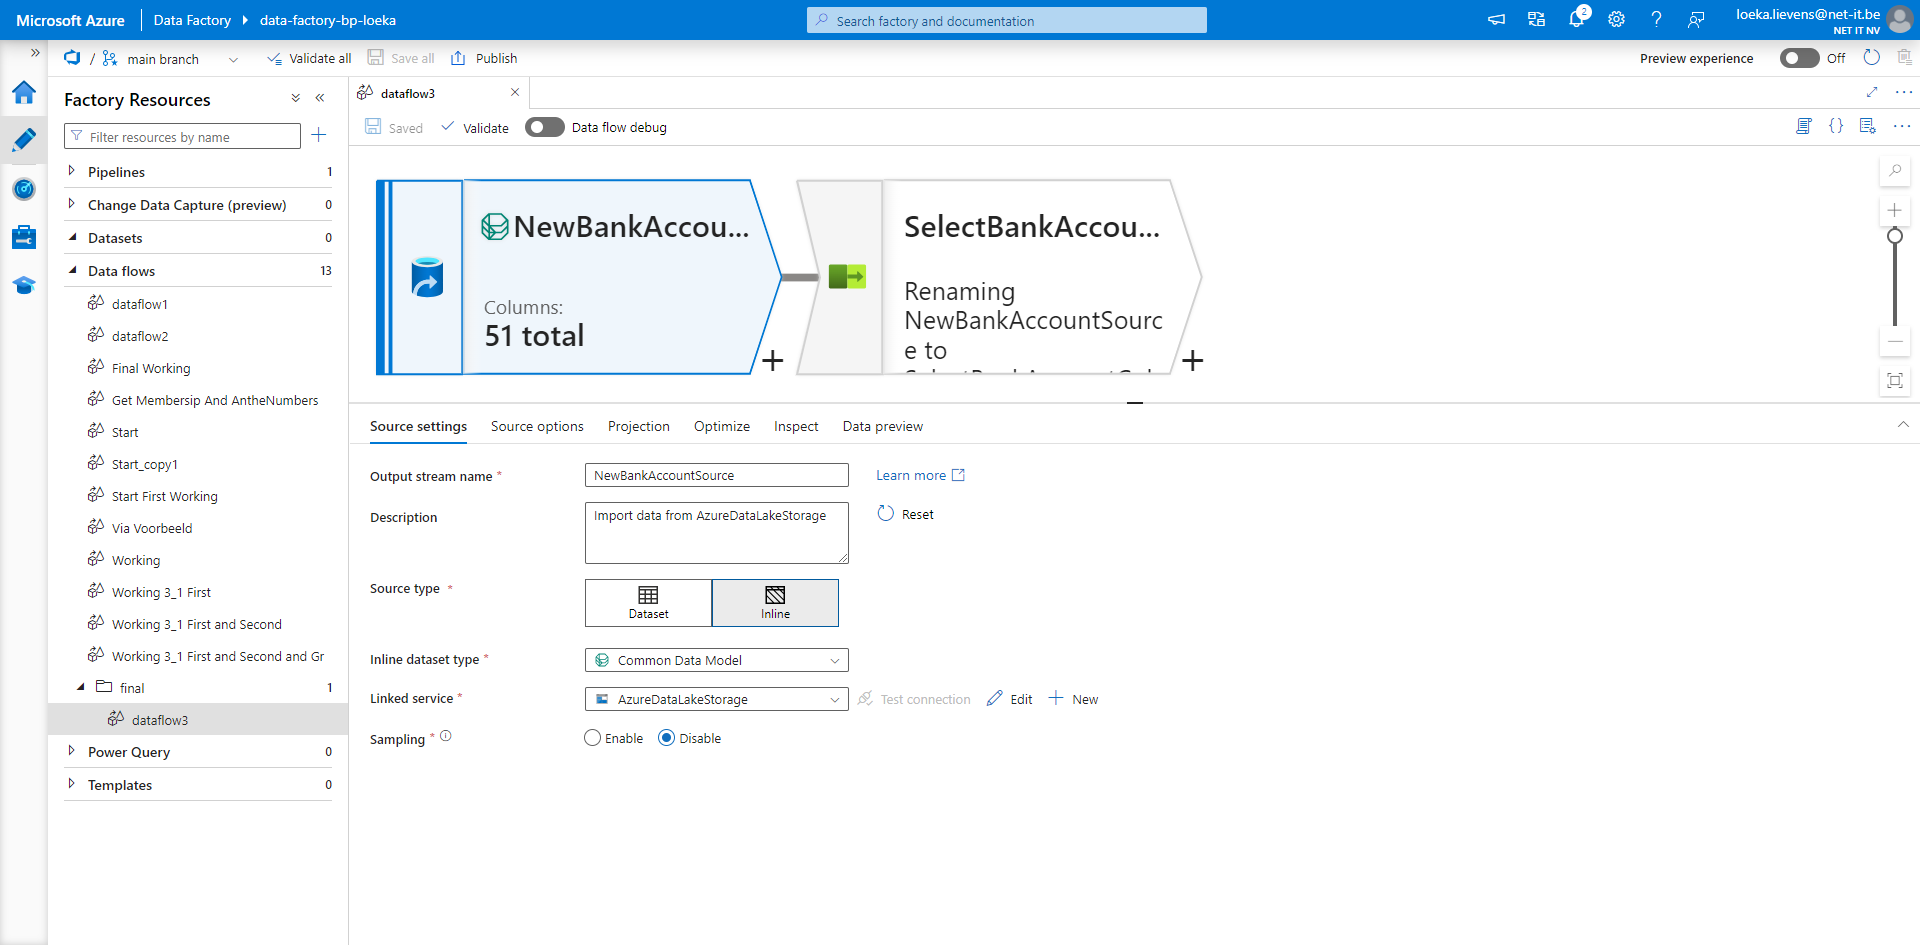
\includegraphics[width=1\textwidth]{./graphics/adf/new_bankaccount_source.png}
%\end{center}
%
%\texttt{Er wordt een source toegevoegd voor de tabel new\_bankaccount.}
%
%\begin{center}
%    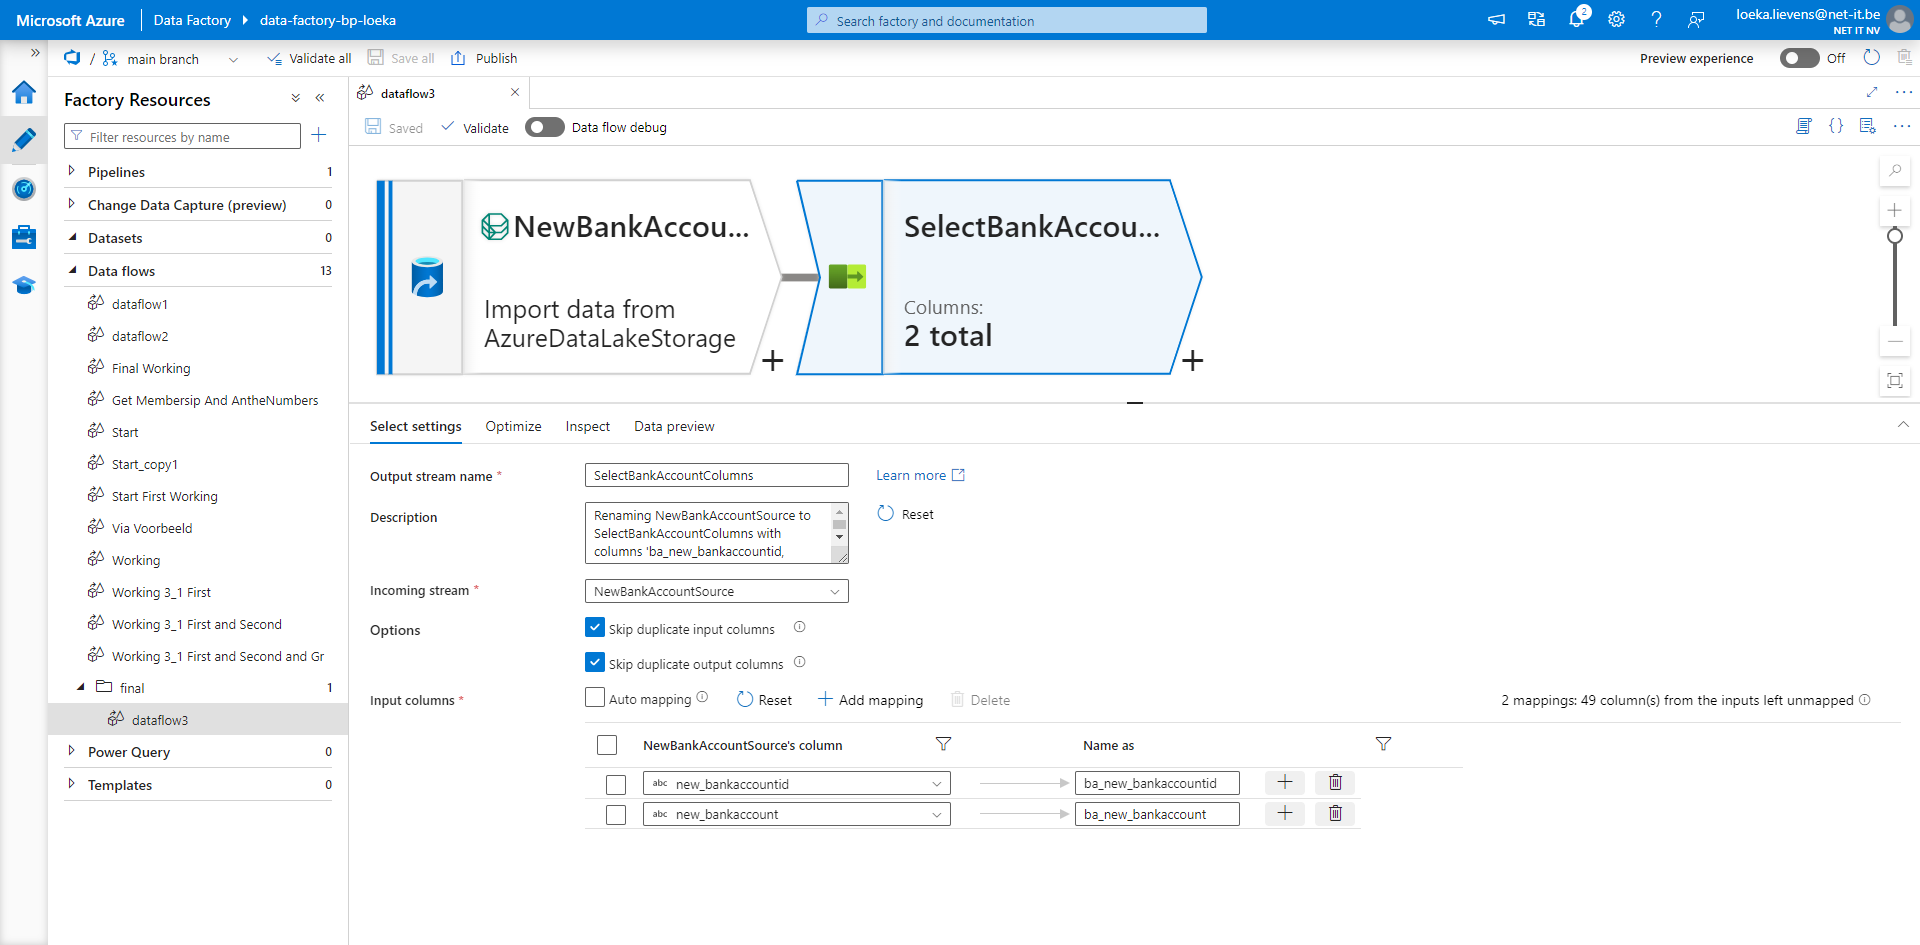
\includegraphics[width=1\textwidth]{./graphics/adf/new_bankaccount_select.png}
%\end{center}
%
%\texttt{De nodige kolommen worden geselecteerd en hernoemt met de prefix `ba\_`.}
%
%\paragraph{\texttt{Tabel new\_year}}
%
%\begin{center}
%    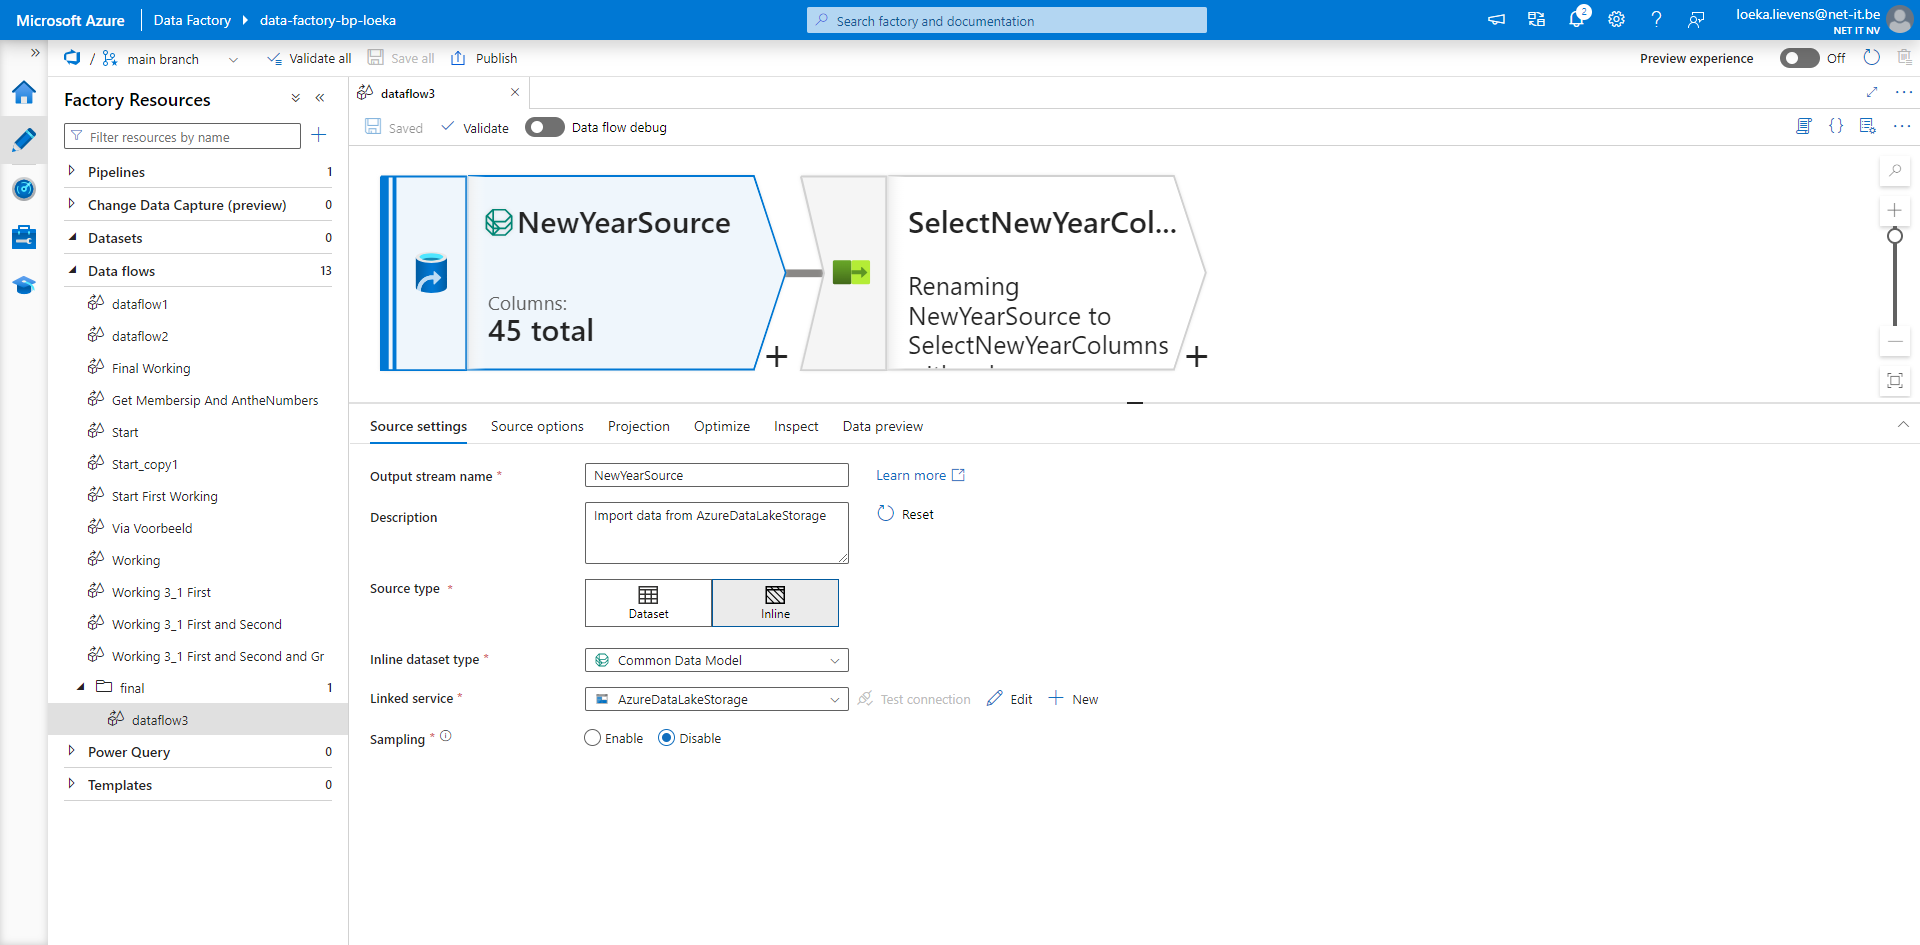
\includegraphics[width=1\textwidth]{./graphics/adf/new_year_source.png}
%\end{center}
%
%\texttt{Er wordt een source toegevoegd voor de tabel new\_year.}
%
%\begin{center}
%    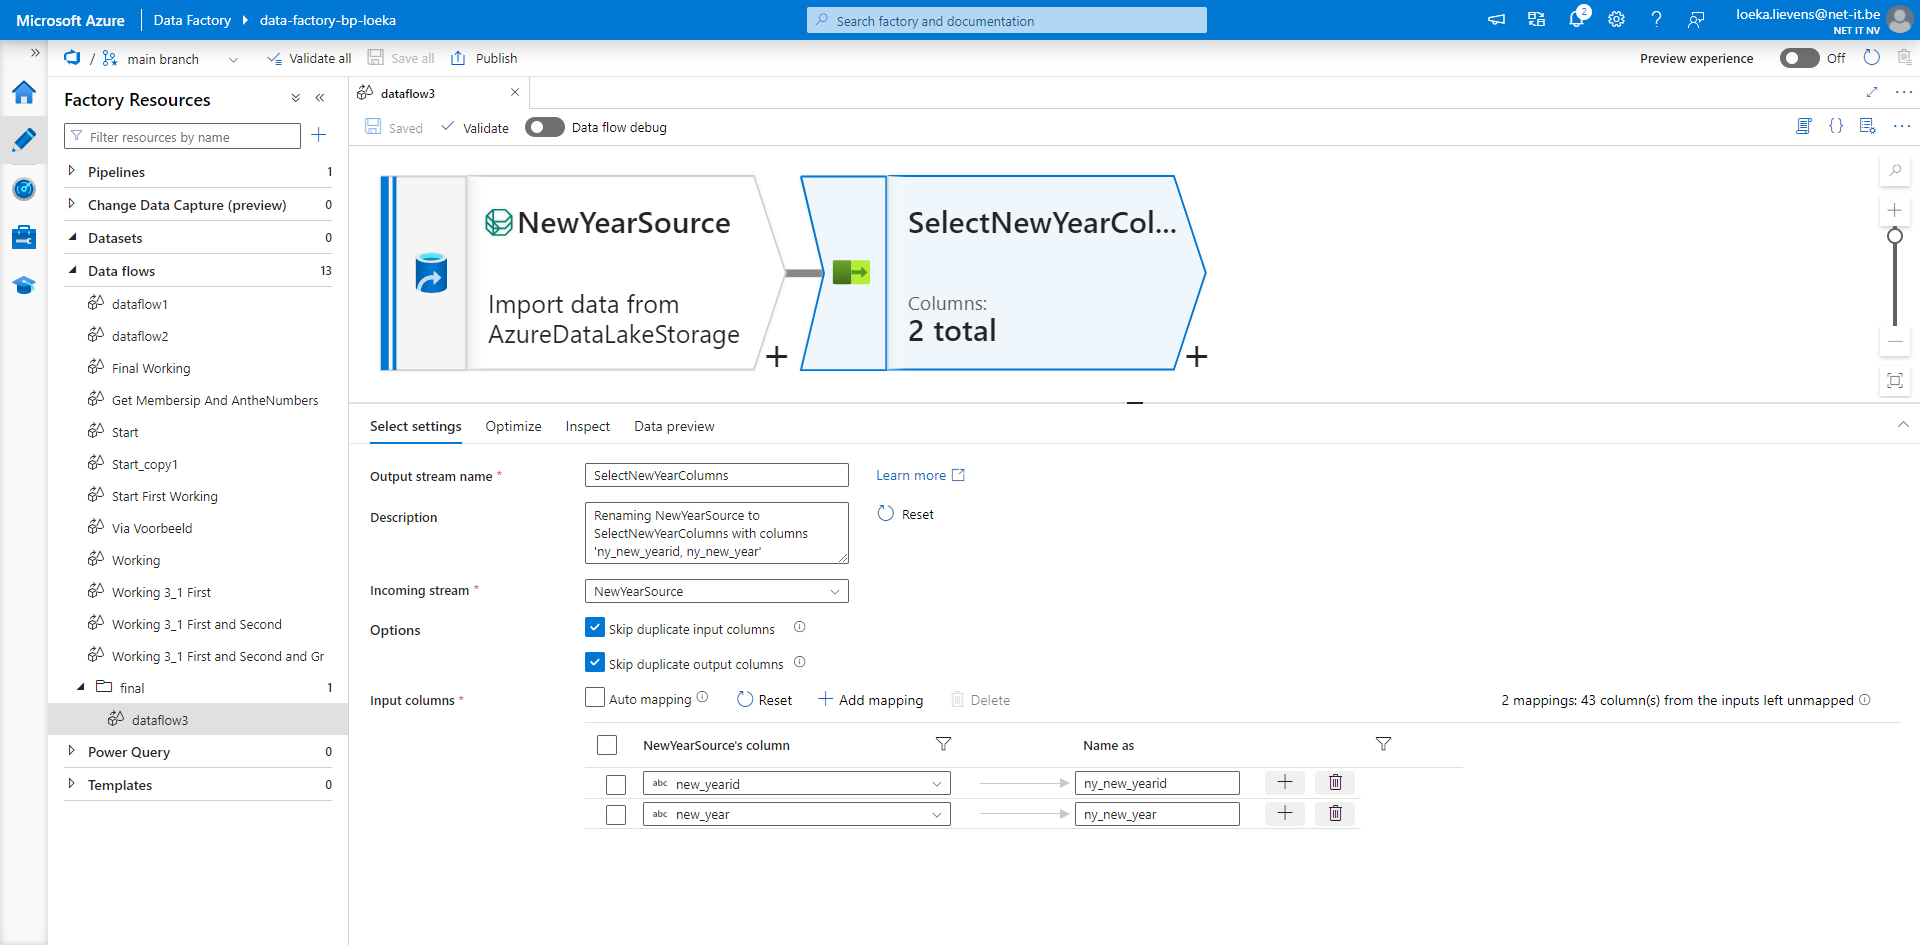
\includegraphics[width=1\textwidth]{./graphics/adf/new_year_select.png}
%\end{center}
%
%\texttt{De nodige kolommen worden geselecteerd en hernoemt met de prefix `ny\_`.}
%
%\paragraph{\texttt{Tabel new\_group}}
%
%\begin{center}
%    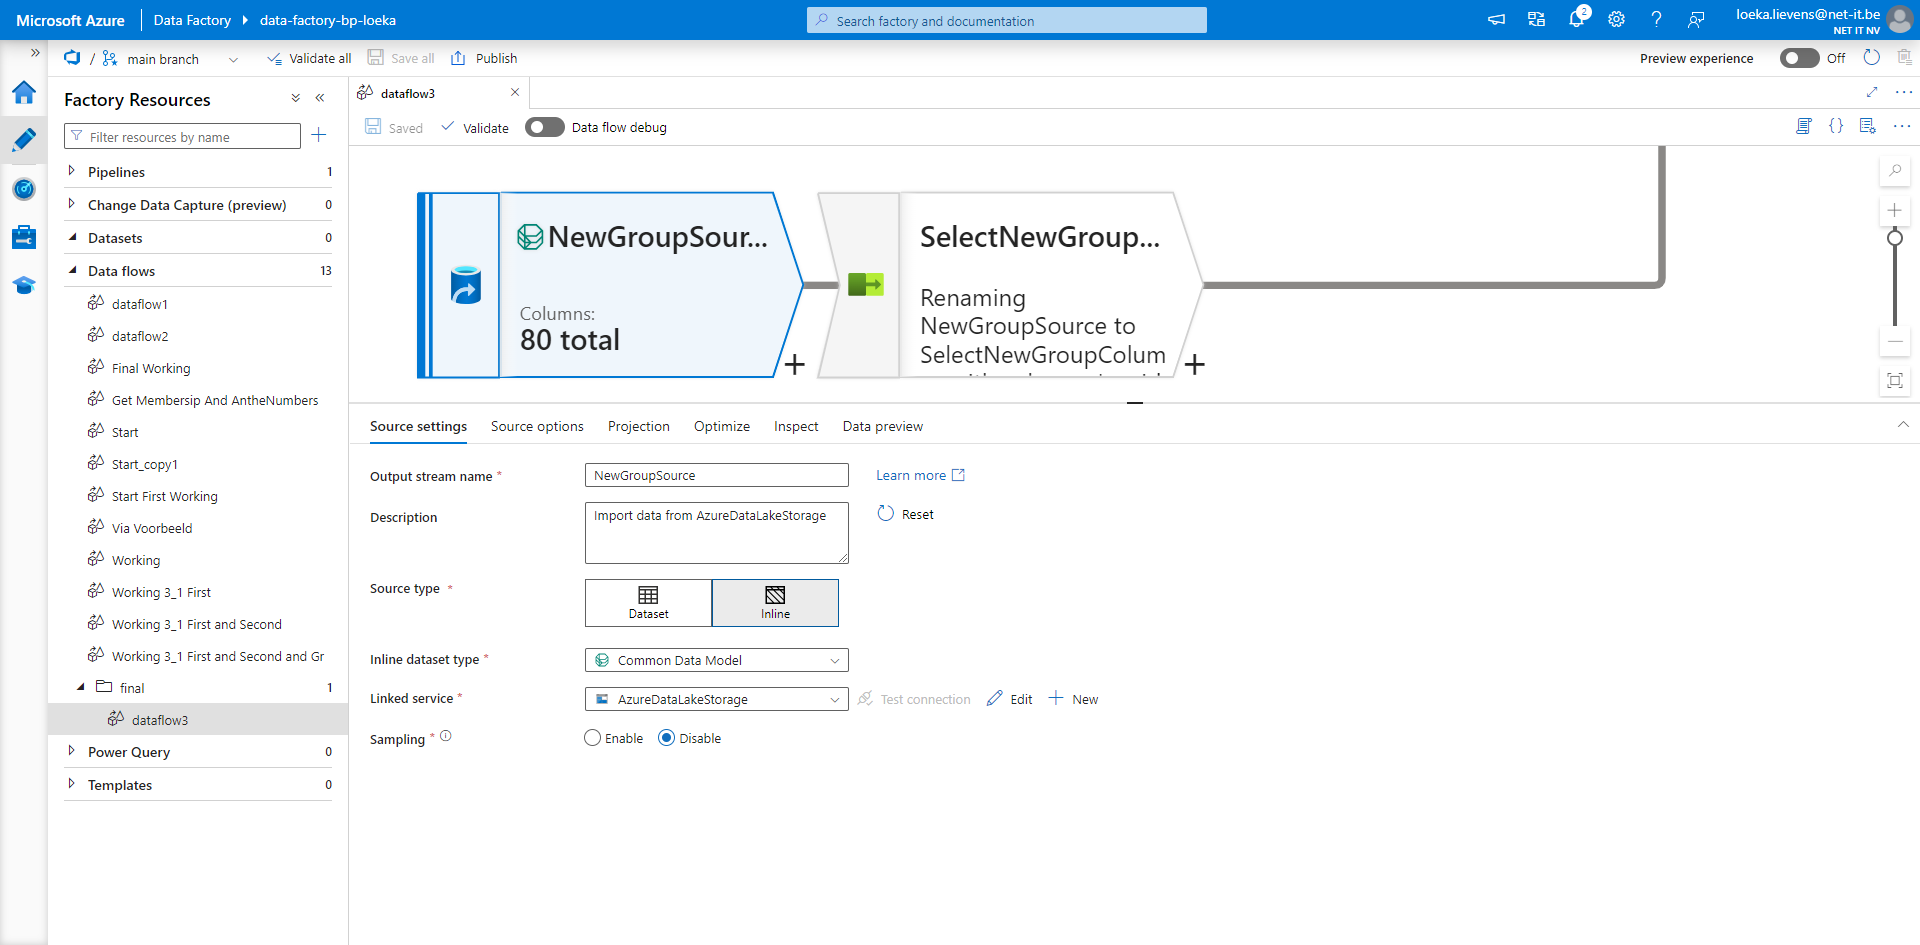
\includegraphics[width=1\textwidth]{./graphics/adf/new_group_source.png}
%\end{center}
%
%\texttt{Er wordt een source toegevoegd voor de tabel new\_group.}
%
%\begin{center}
%    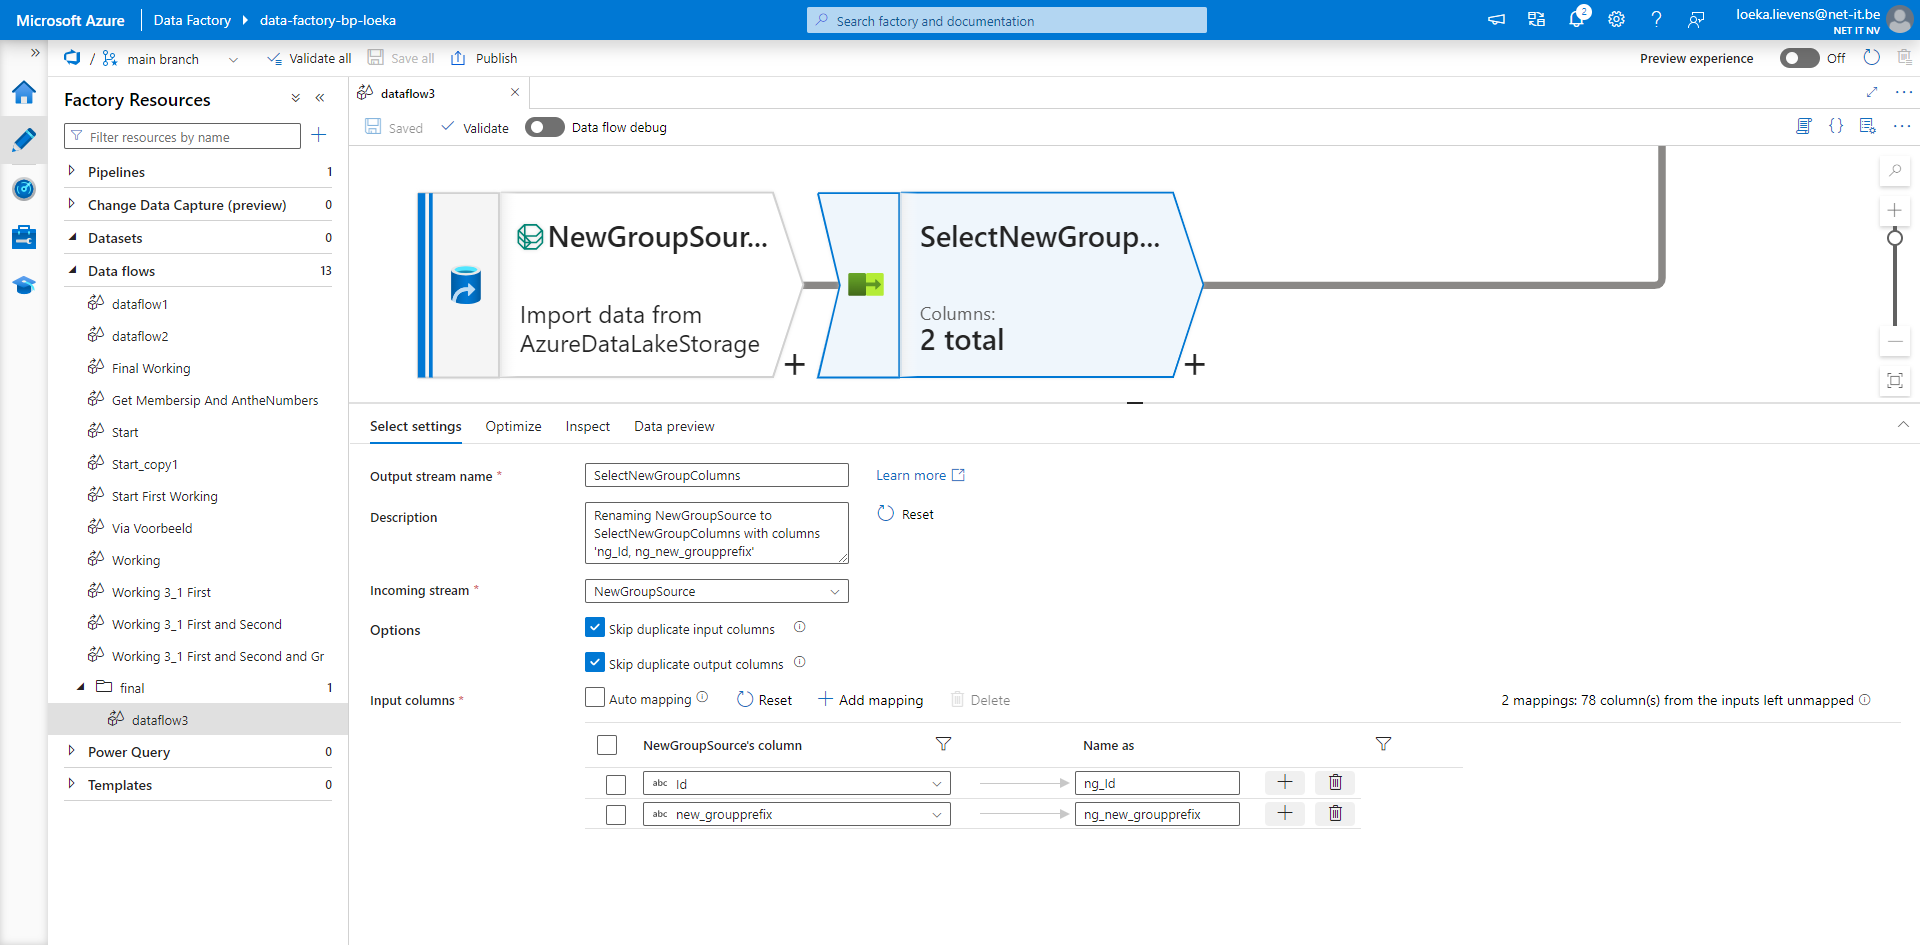
\includegraphics[width=1\textwidth]{./graphics/adf/new_group_select.png}
%\end{center}
%
%\texttt{De nodige kolommen worden geselecteerd en hernoemt met de prefix `ng\_`.}
%
%\paragraph{\texttt{Tabel new\_organizationyear}}
%
%\begin{center}
%    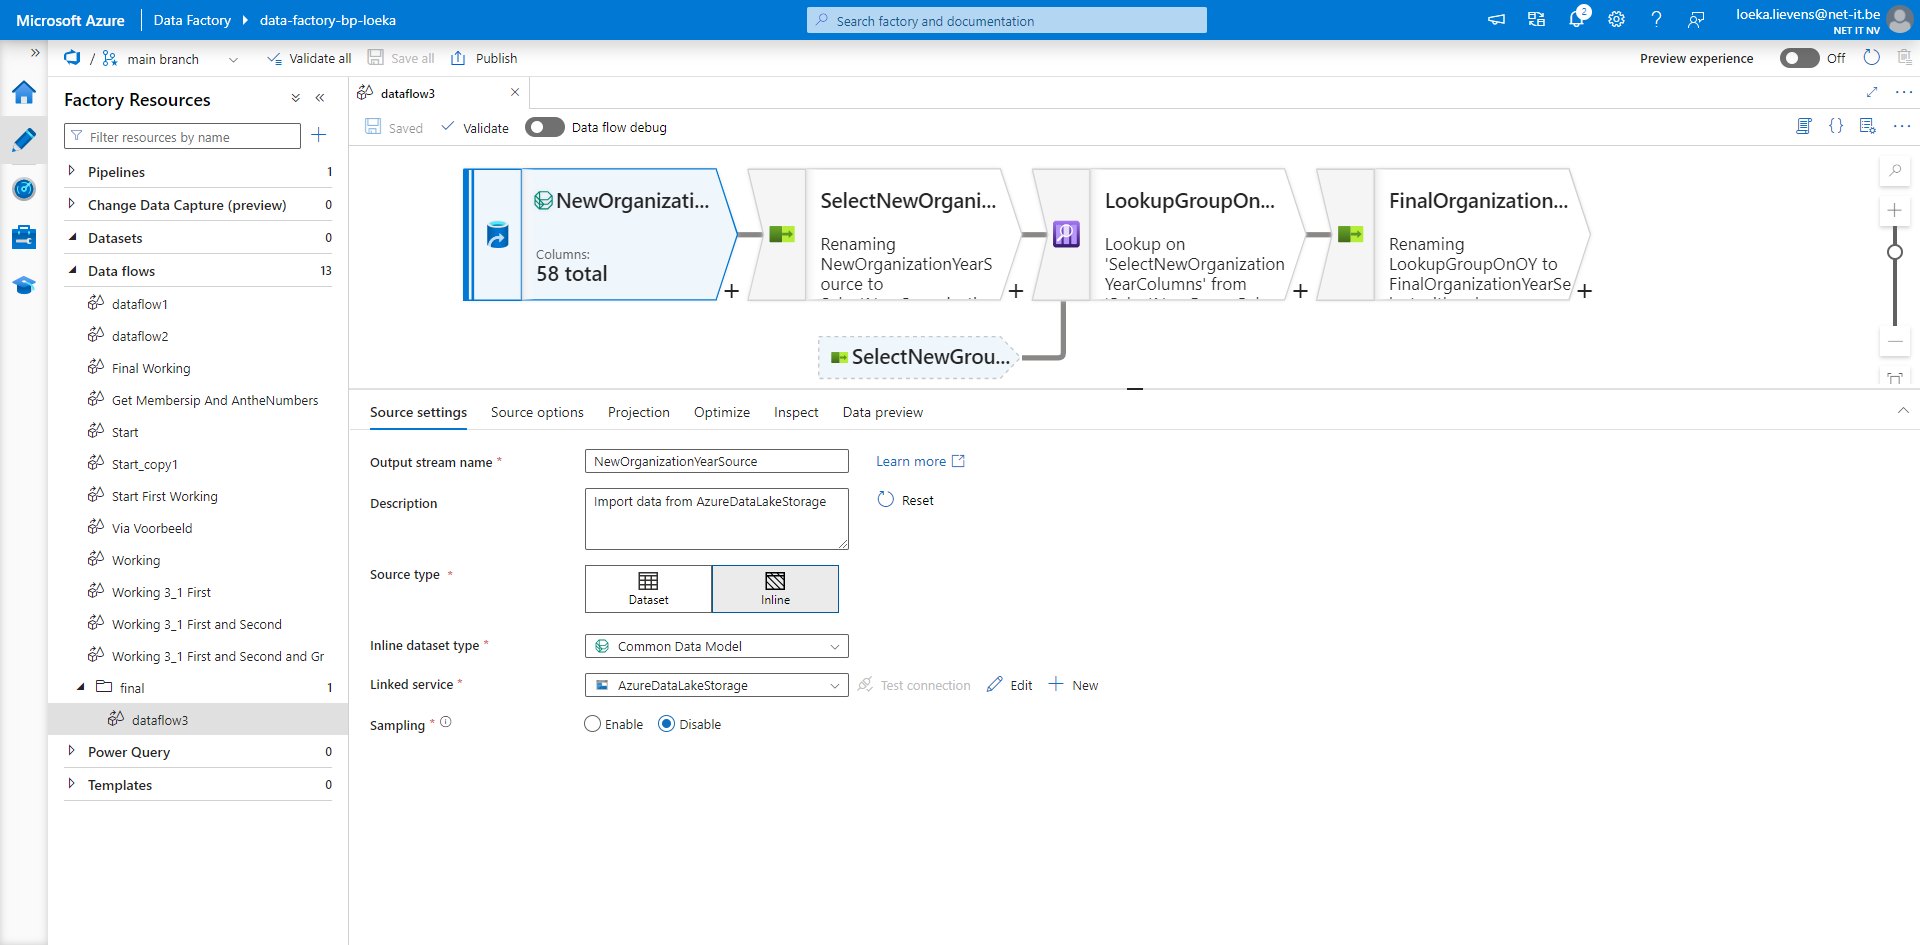
\includegraphics[width=1\textwidth]{./graphics/adf/new_organizationyear_source.png}
%\end{center}
%
%\texttt{Er wordt een source toegevoegd voor de tabel new\_organizationyear.}
%
%\begin{center}
%    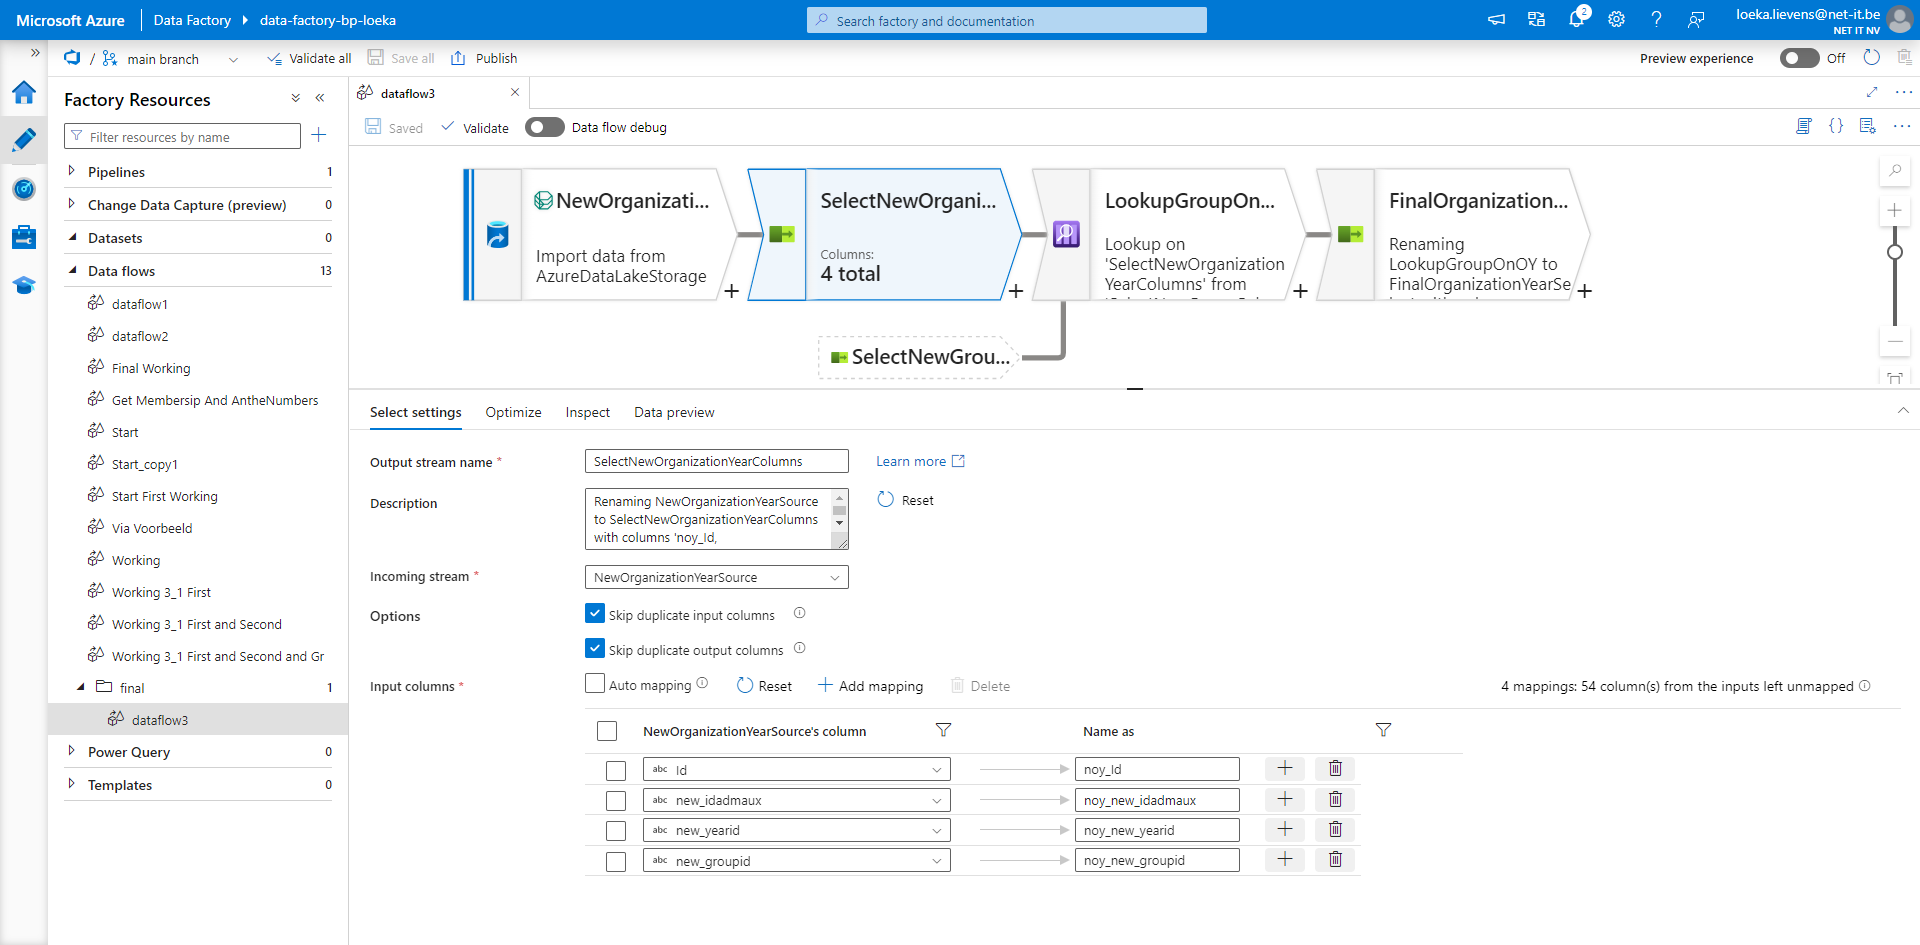
\includegraphics[width=1\textwidth]{./graphics/adf/new_organizationyear_select.png}
%\end{center}
%
%\texttt{De nodige kolommen worden geselecteerd en hernoemt met de prefix `noy\_`.}
%
%\begin{center}
%    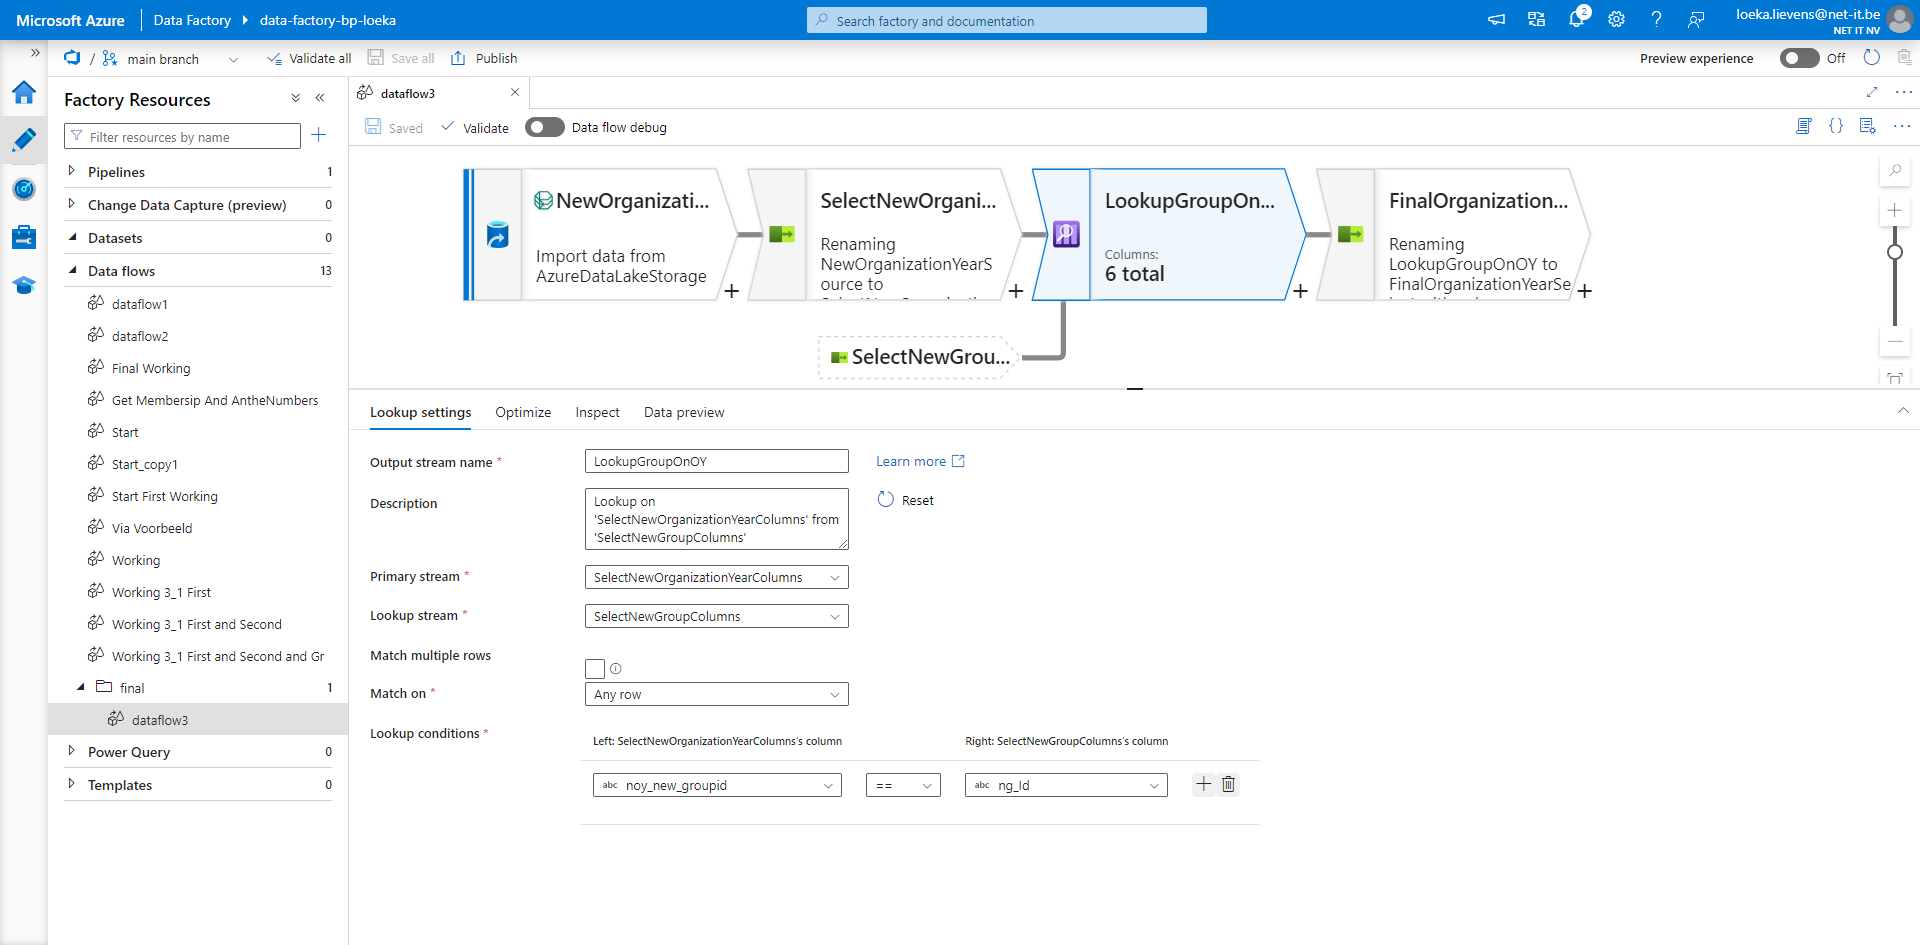
\includegraphics[width=1\textwidth]{./graphics/adf/new_organizationyear_lookup.png}
%\end{center}
%
%\texttt{De tabel new\_group wordt gejoind met een lookup aan de hand van id.}
%
%% TODO: Link naar juiste foto?
%
%\begin{center}
%    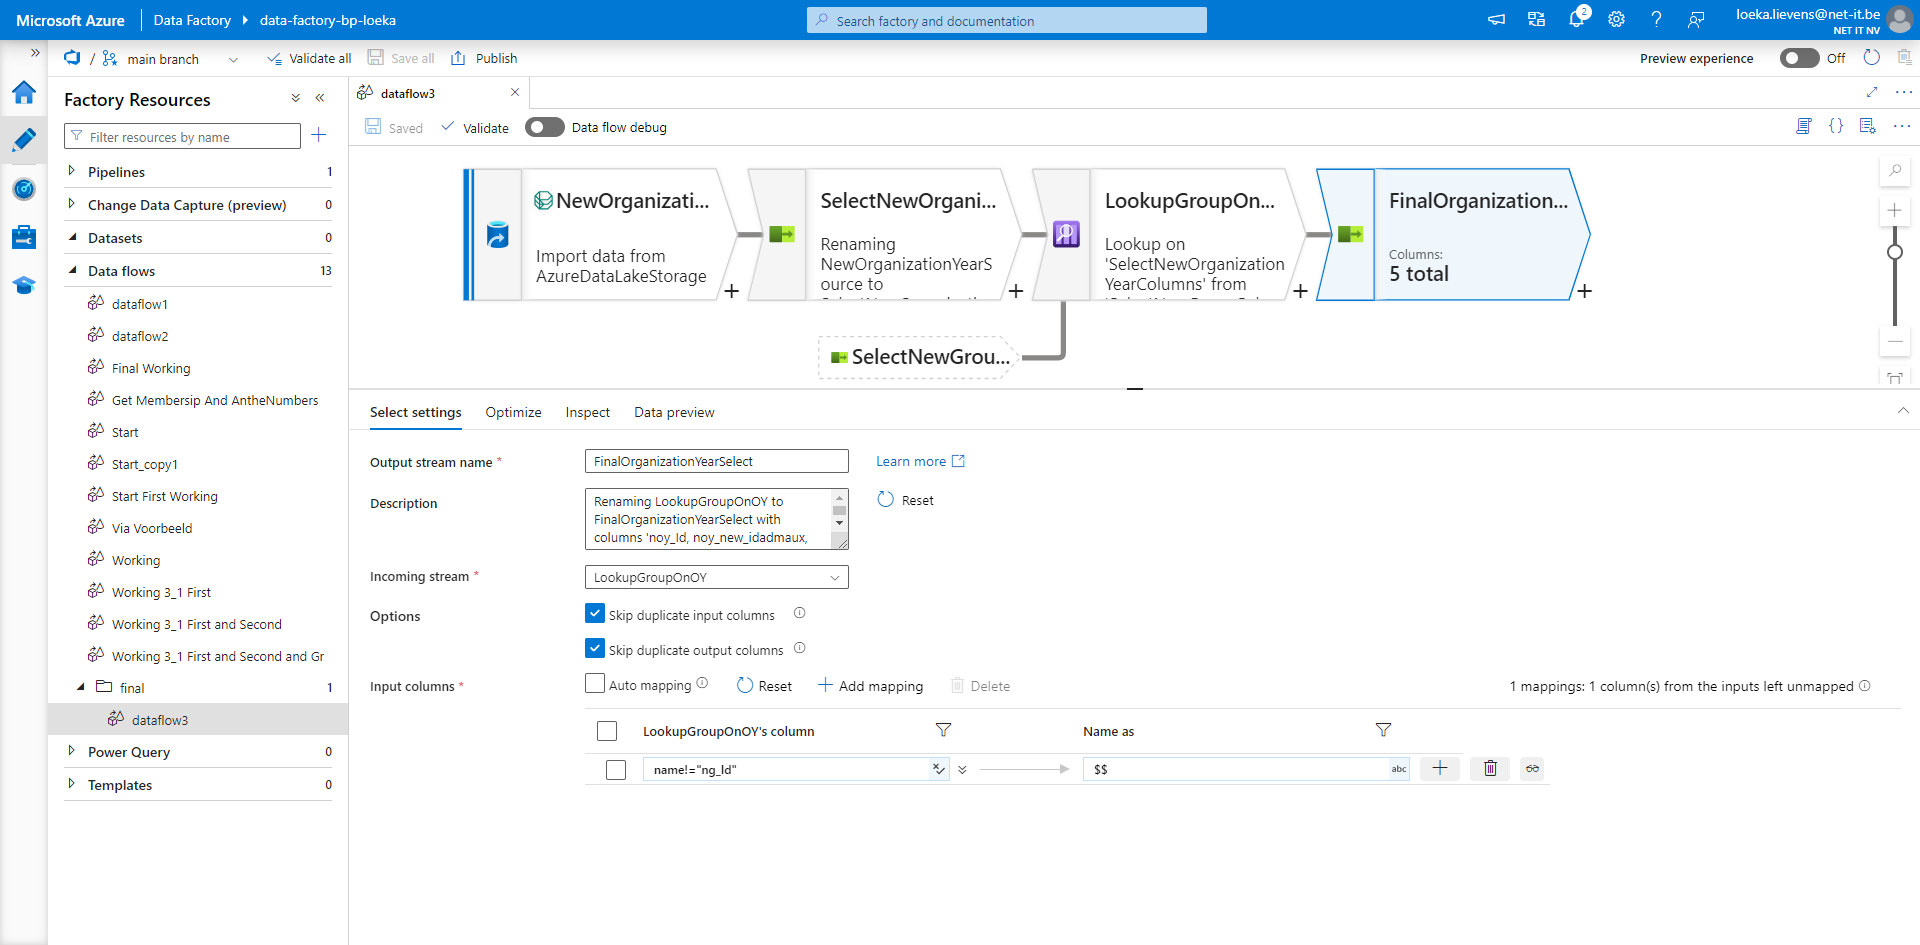
\includegraphics[width=1\textwidth]{./graphics/adf/new_organizationyear_final.png}
%\end{center}
%
%\texttt{We selecteren alle kolommen behalve de kolom met naam ng\_id aangezien deze steeds hetzelfde zal zijn als noy\_new\_groupid.}
%
%\paragraph{\texttt{Tabel new\_membership}}
%
%\begin{center}
%    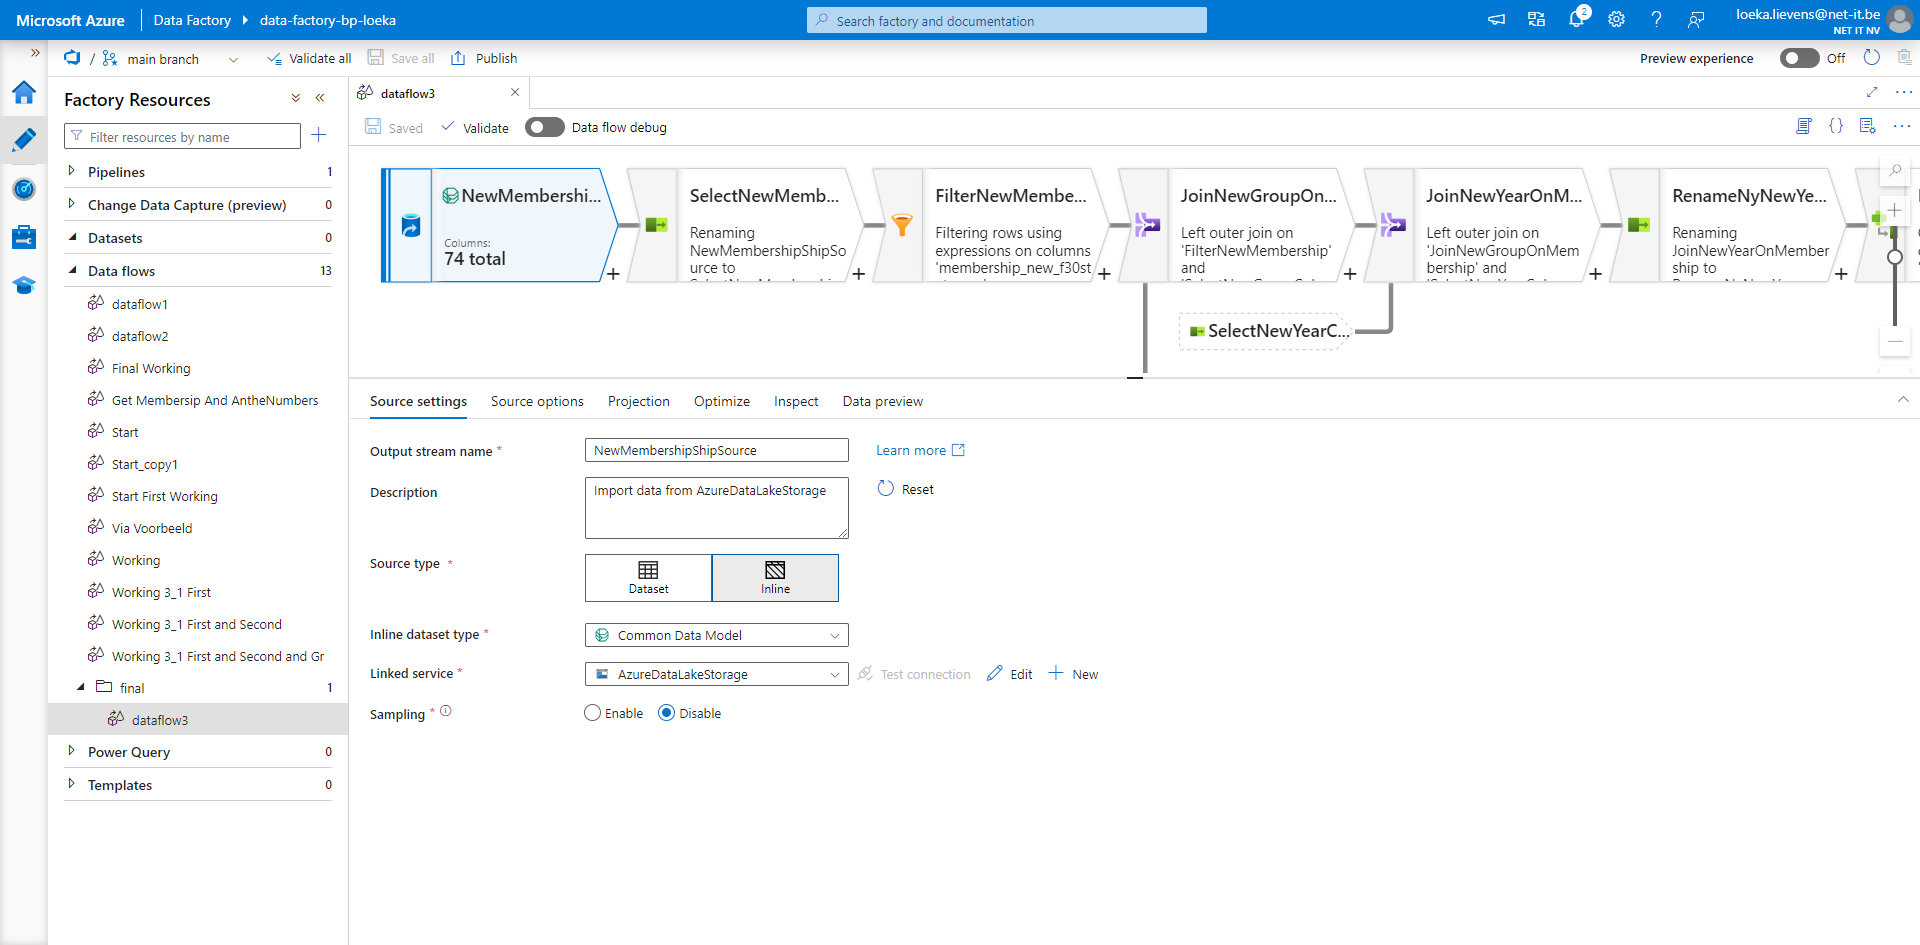
\includegraphics[width=1\textwidth]{./graphics/adf/new_membership_source.png}
%\end{center}
%
%\texttt{Er wordt een source toegevoegd voor de tabel new\_membership.}
%
%\begin{center}
%    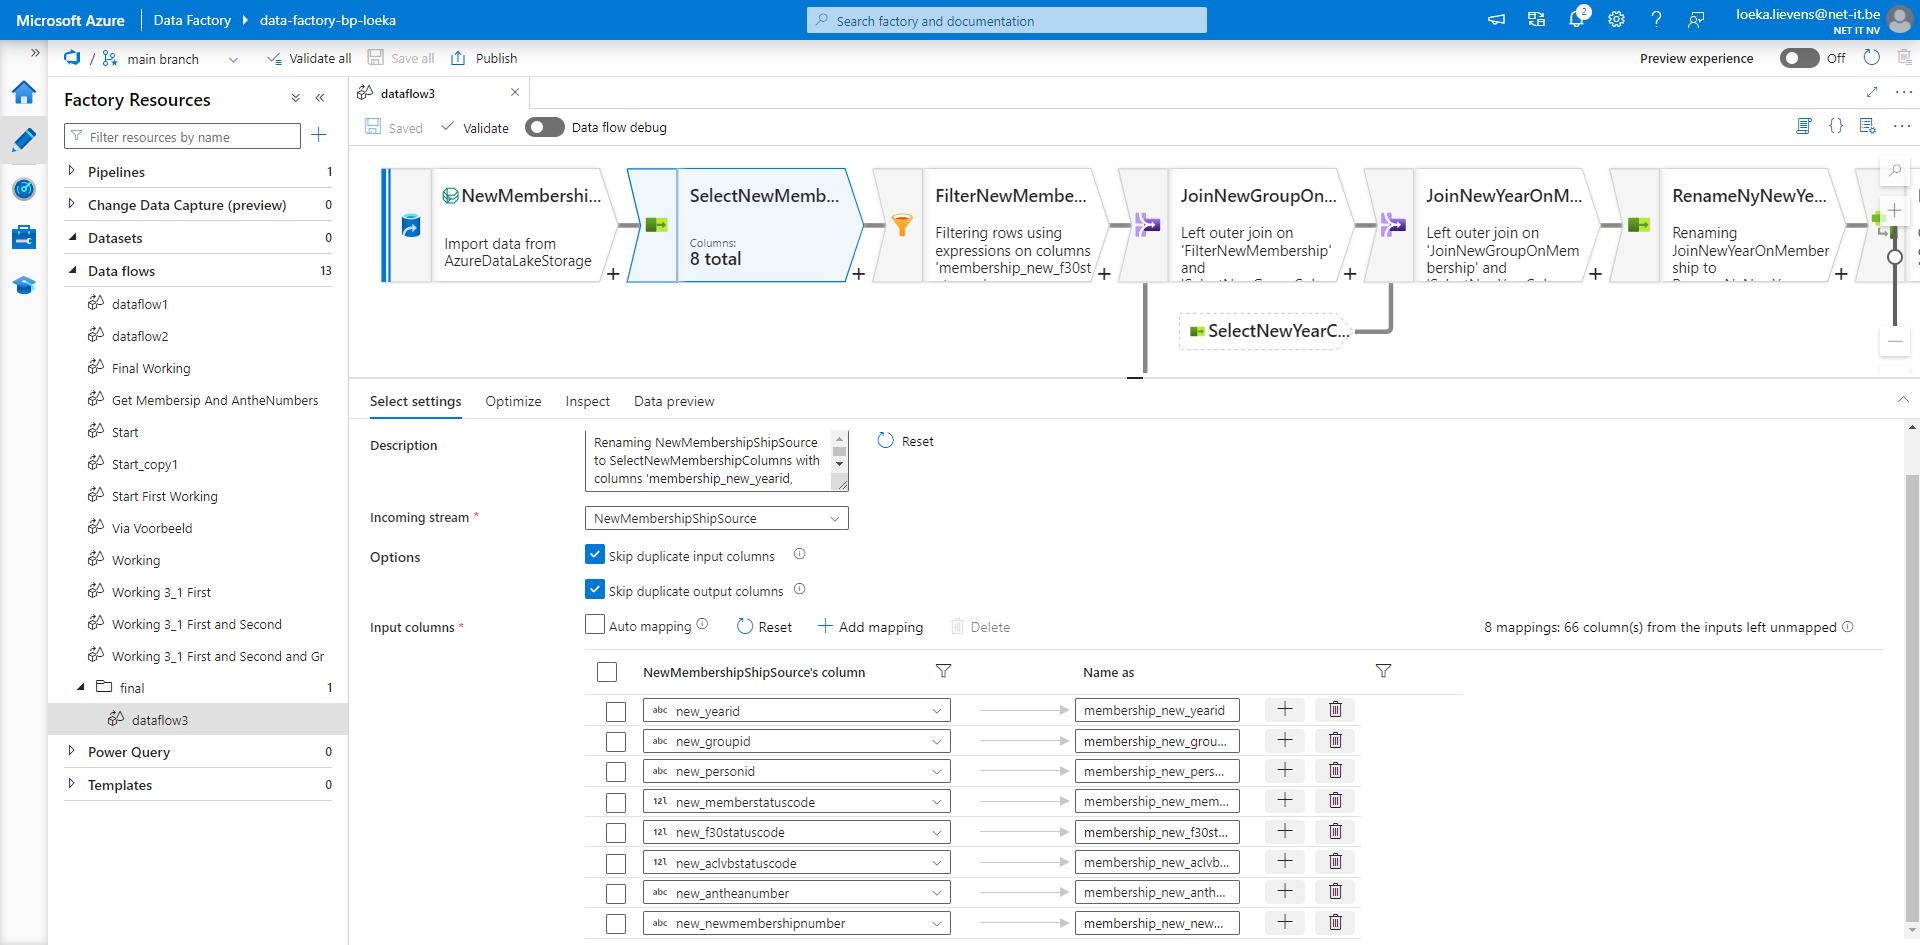
\includegraphics[width=1\textwidth]{./graphics/adf/new_membership_select.png}
%\end{center}
%
%\texttt{De nodige kolommen worden geselecteerd en hernoemt met de prefix `membership\_`.}
%
%\begin{center}
%    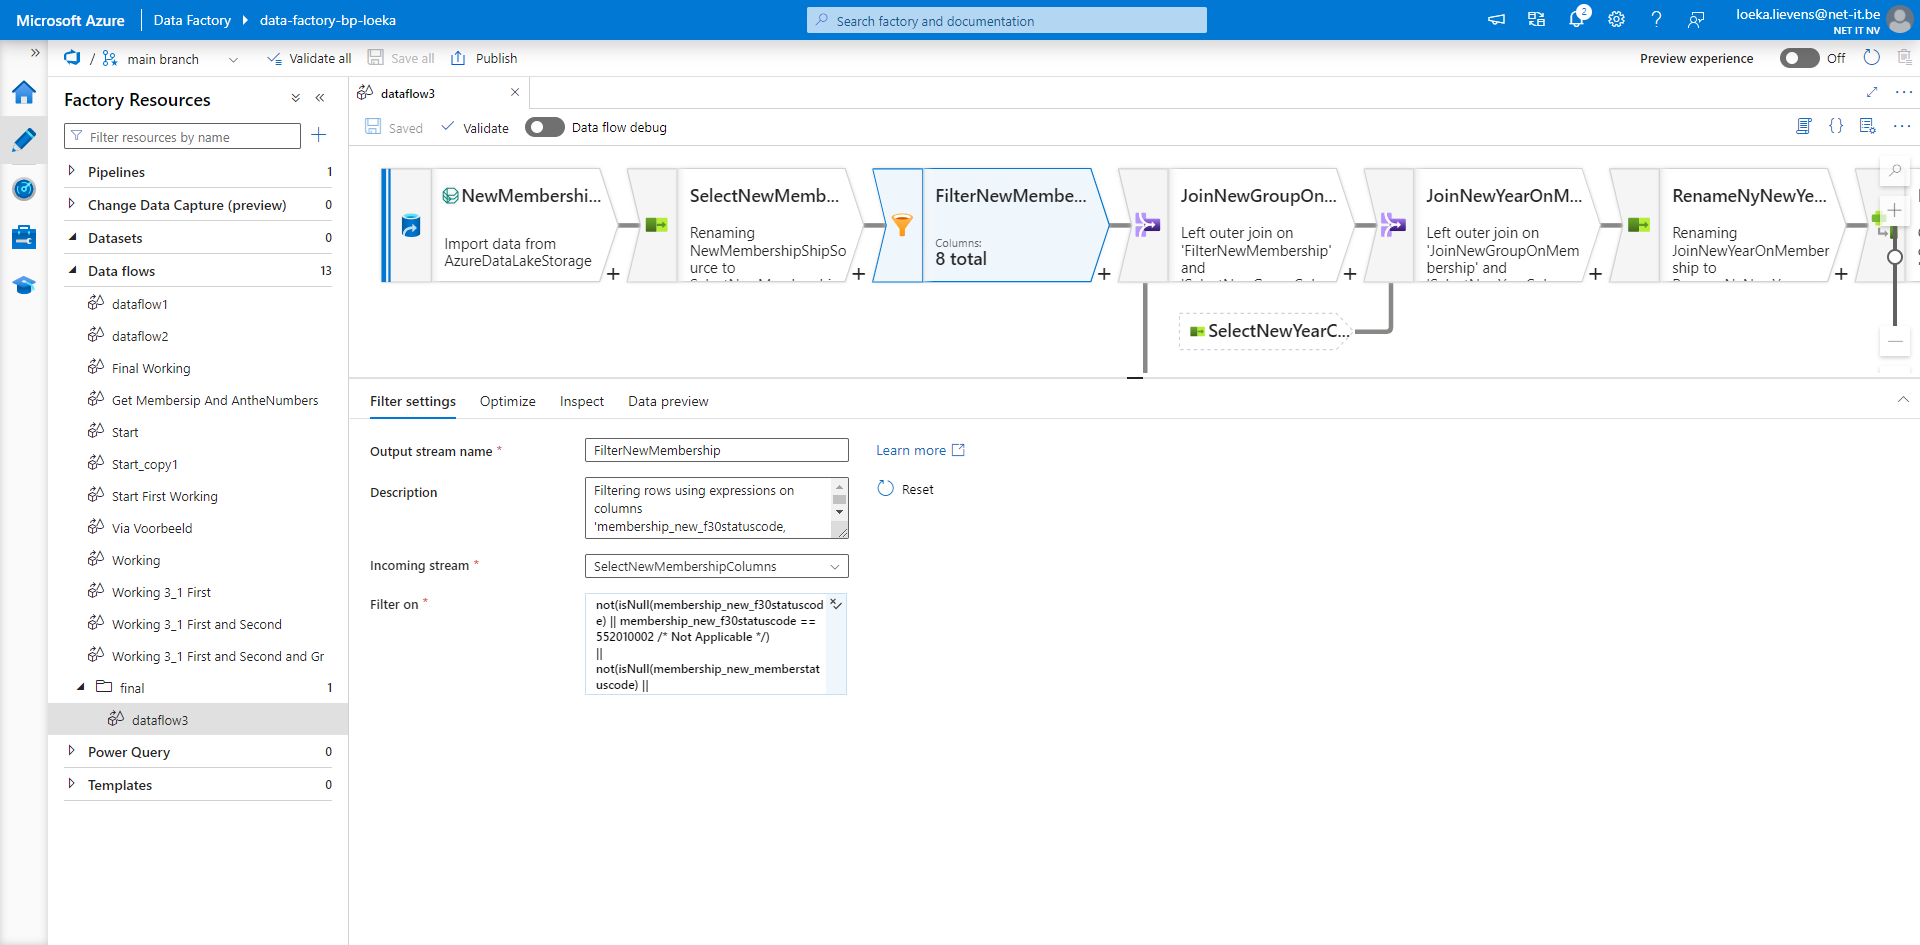
\includegraphics[width=1\textwidth]{./graphics/adf/new_membership_filter_1.png}
%\end{center}
%
%\begin{center}
%    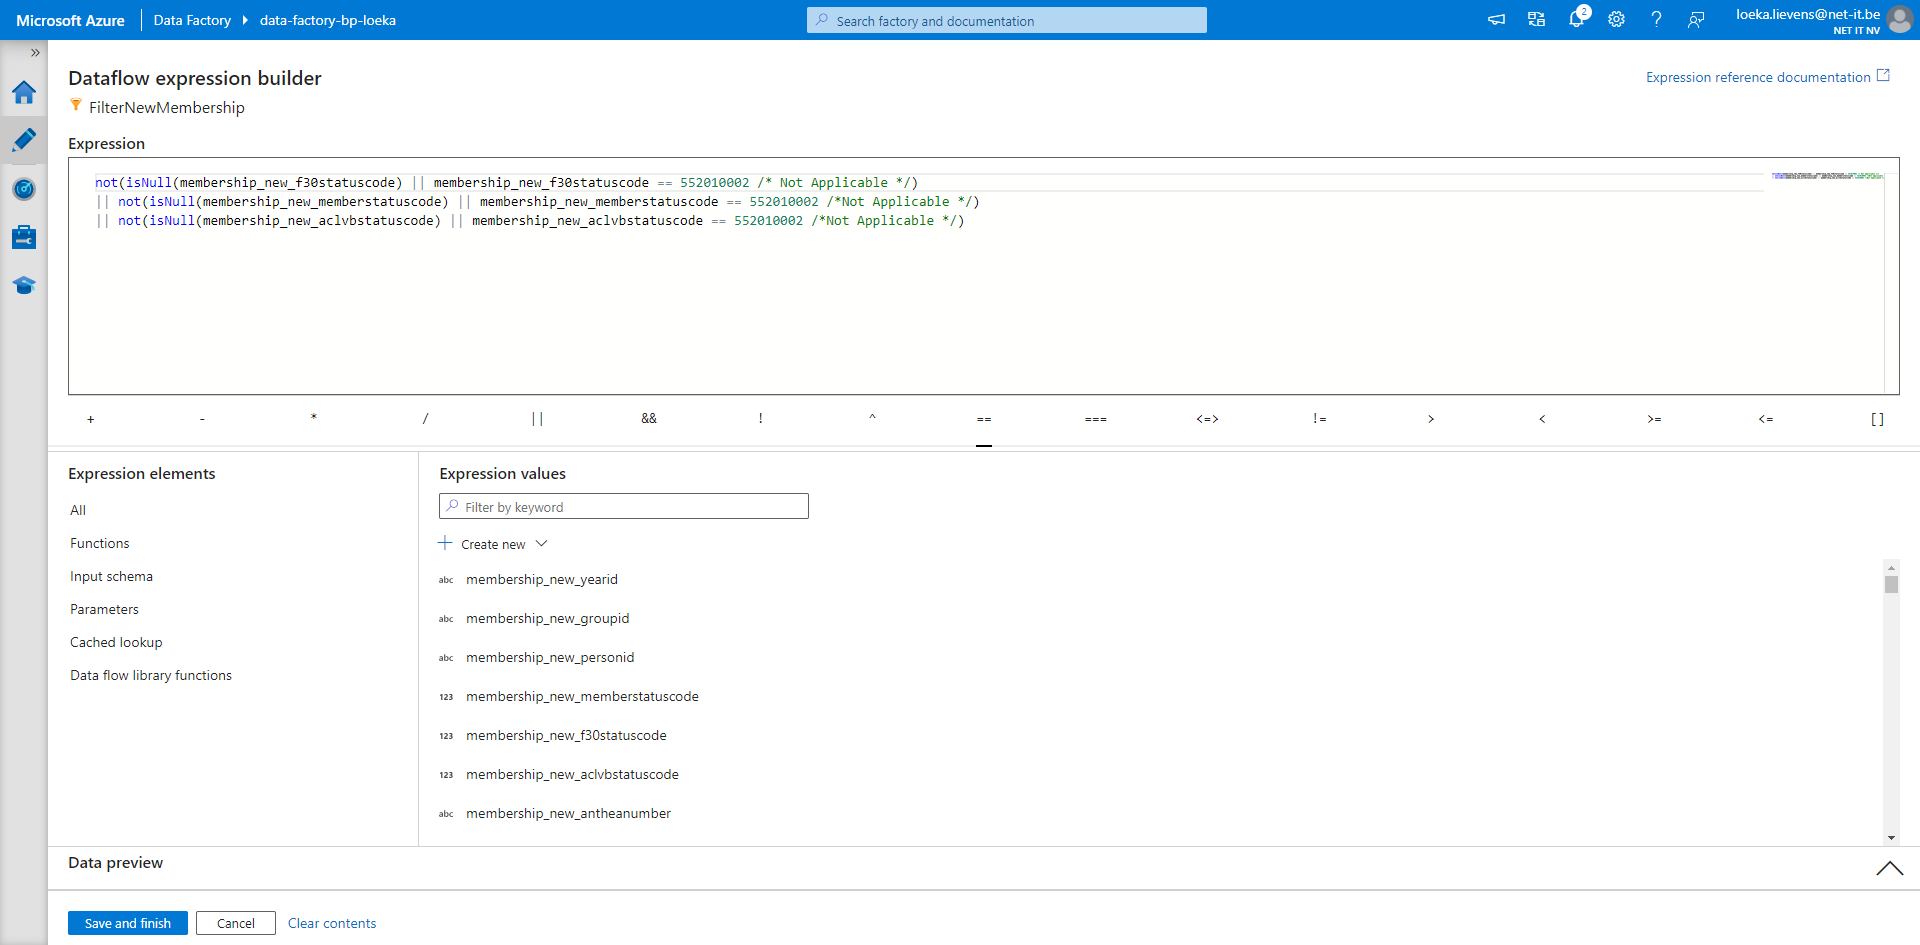
\includegraphics[width=1\textwidth]{./graphics/adf/new_membership_filter_2.png}
%\end{center}
%
%\texttt{De membership records worden gefilterd aan de hand van `new\_f30statuscode`, `new\_memberstatuscode` en `new\_aclvbstatuscode`.}
%
%\begin{center}
%    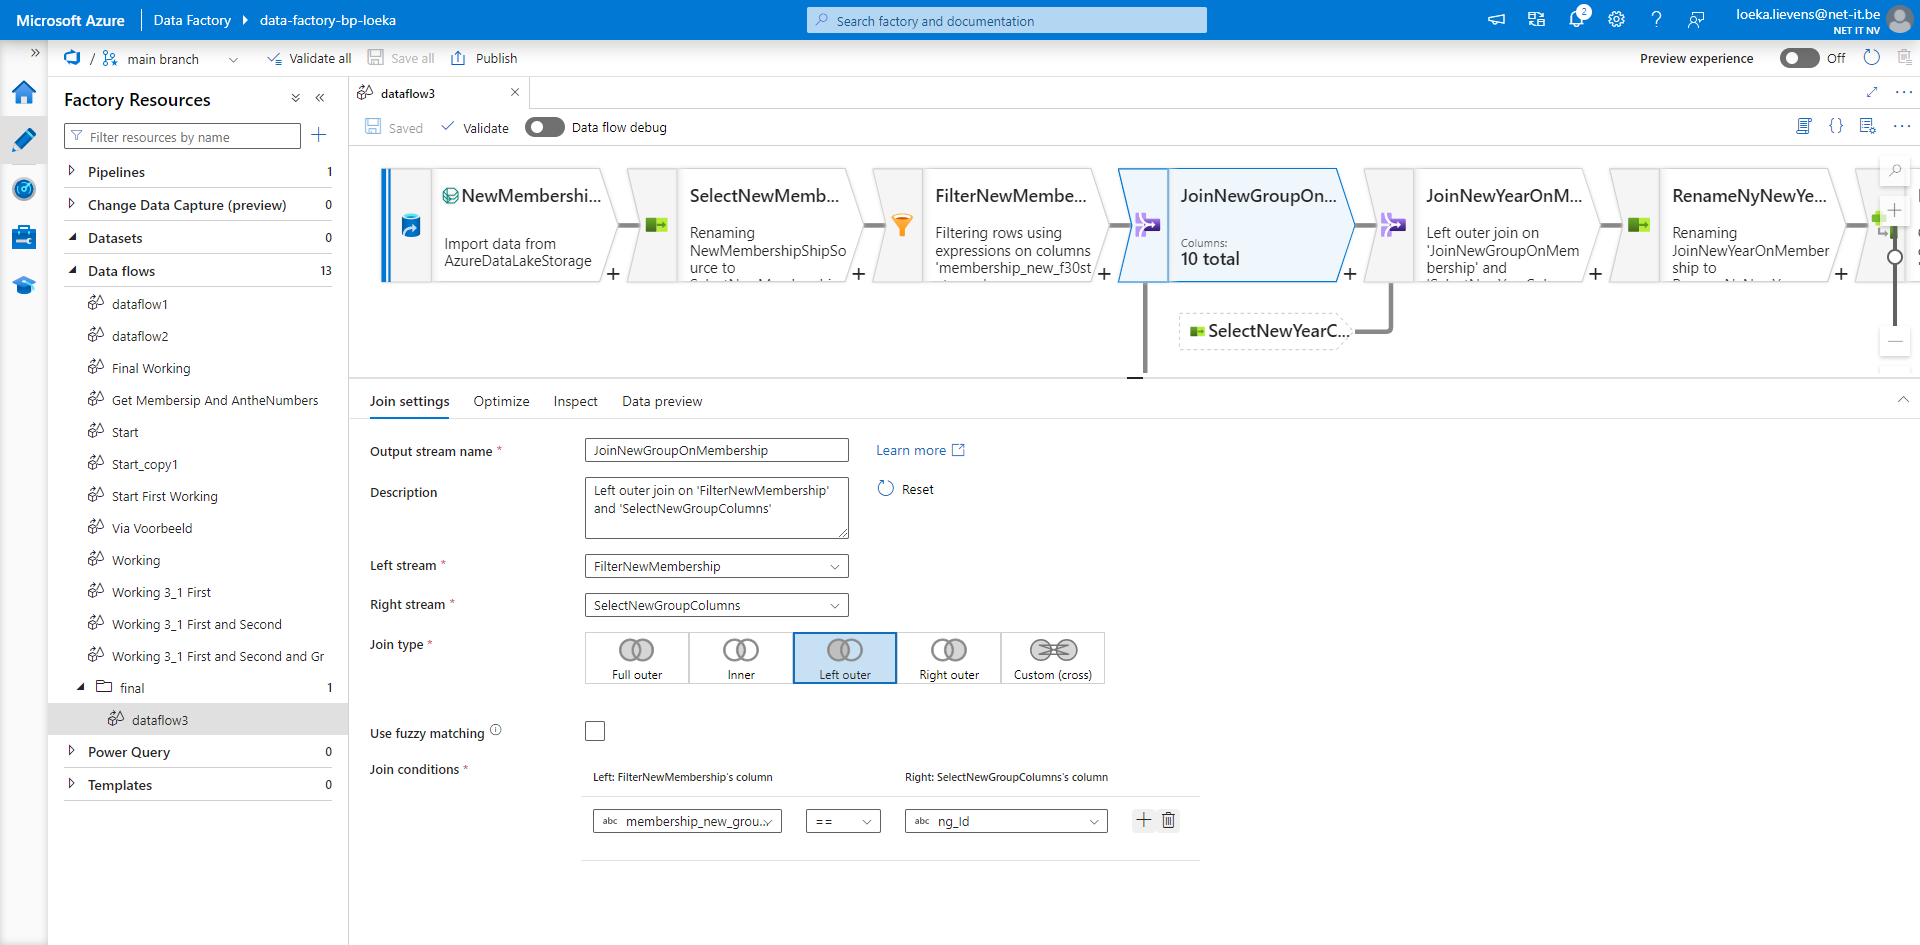
\includegraphics[width=1\textwidth]{./graphics/adf/new_membership_join_1.png}
%\end{center}
%
%\texttt{De tabel new\_group wordt gejoind aan de hand van id.}
%
%\begin{center}
%    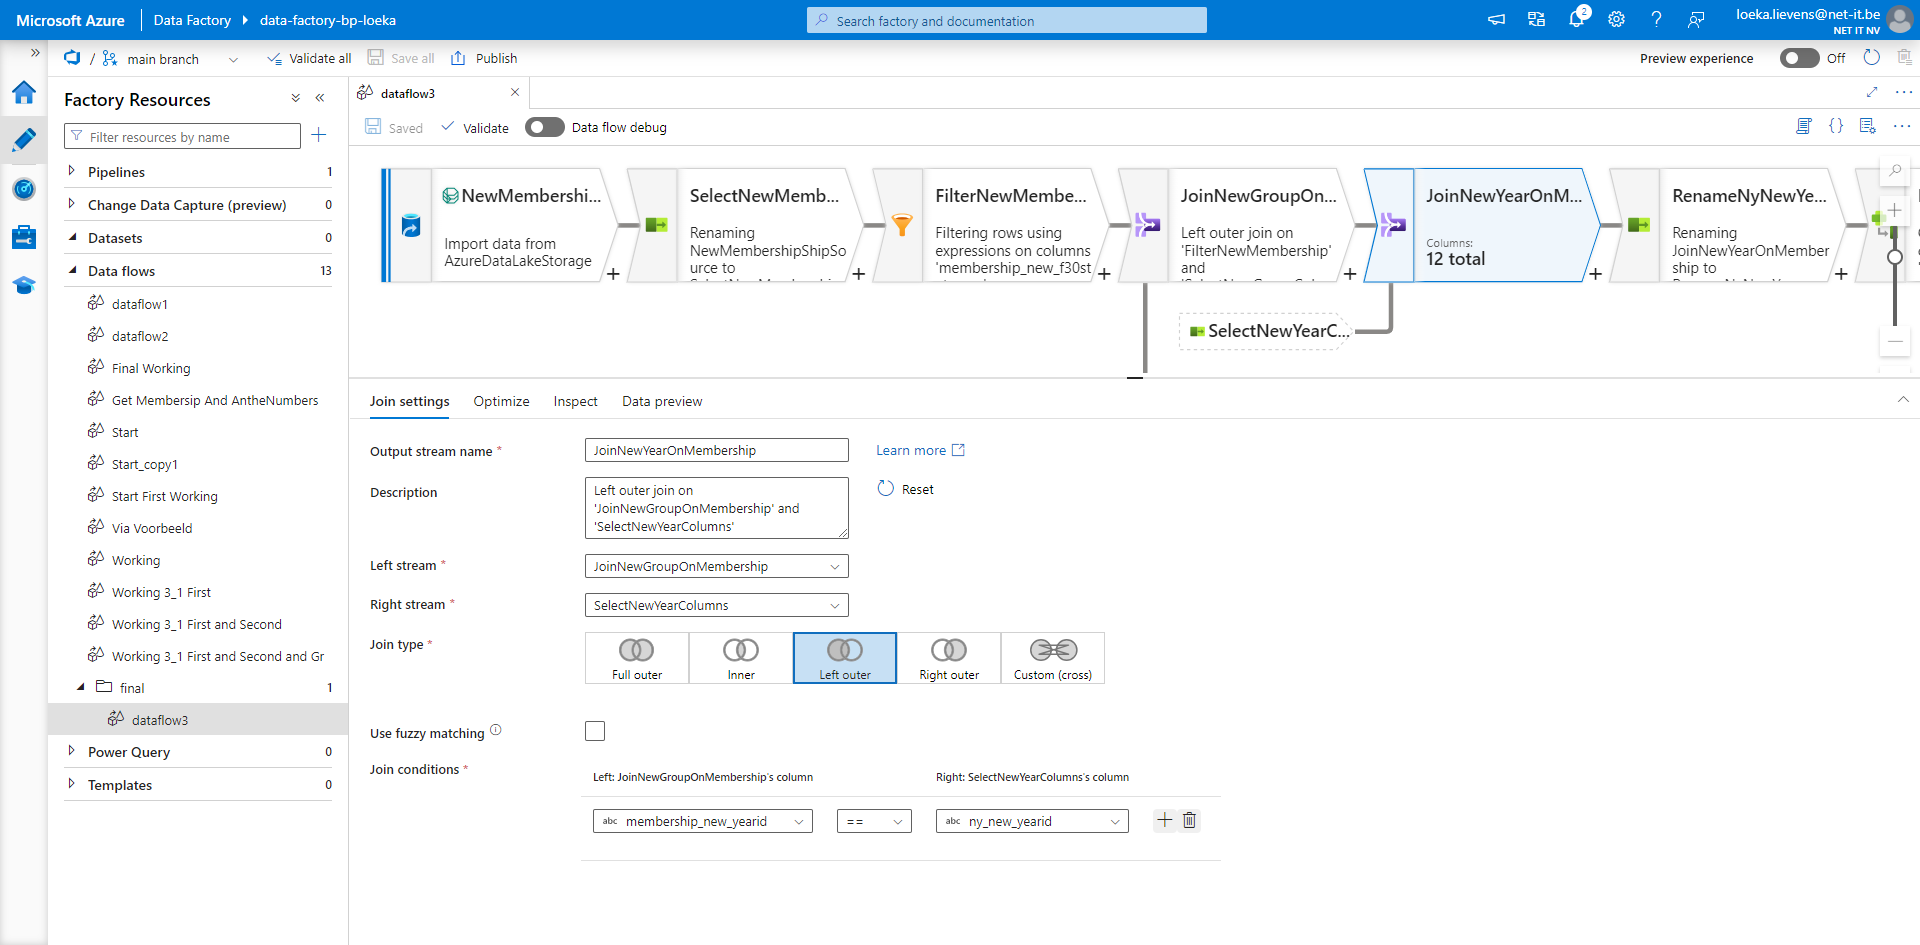
\includegraphics[width=1\textwidth]{./graphics/adf/new_membership_join_2.png}
%\end{center}
%
%\texttt{De tabel new\_year wordt gejoind aan de hand van id.}
%
%\begin{center}
%    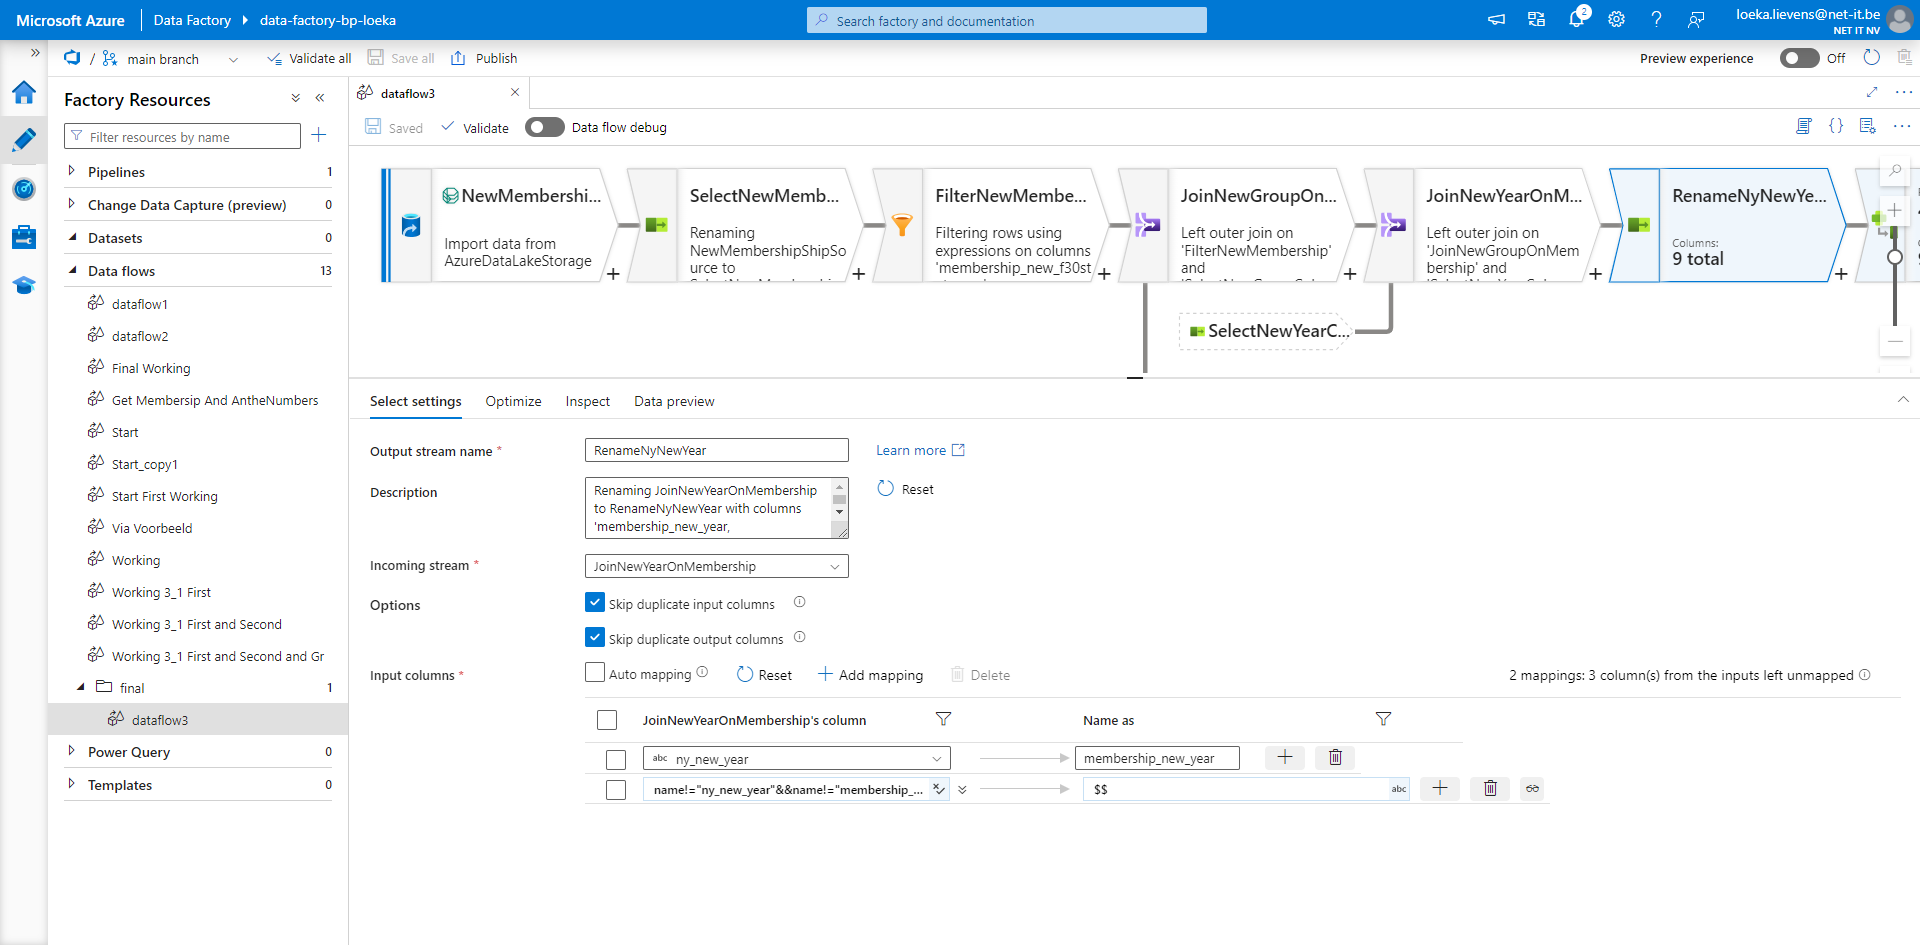
\includegraphics[width=1\textwidth]{./graphics/adf/new_membership_secondselect_1.png}
%\end{center}
%
%\begin{center}
%    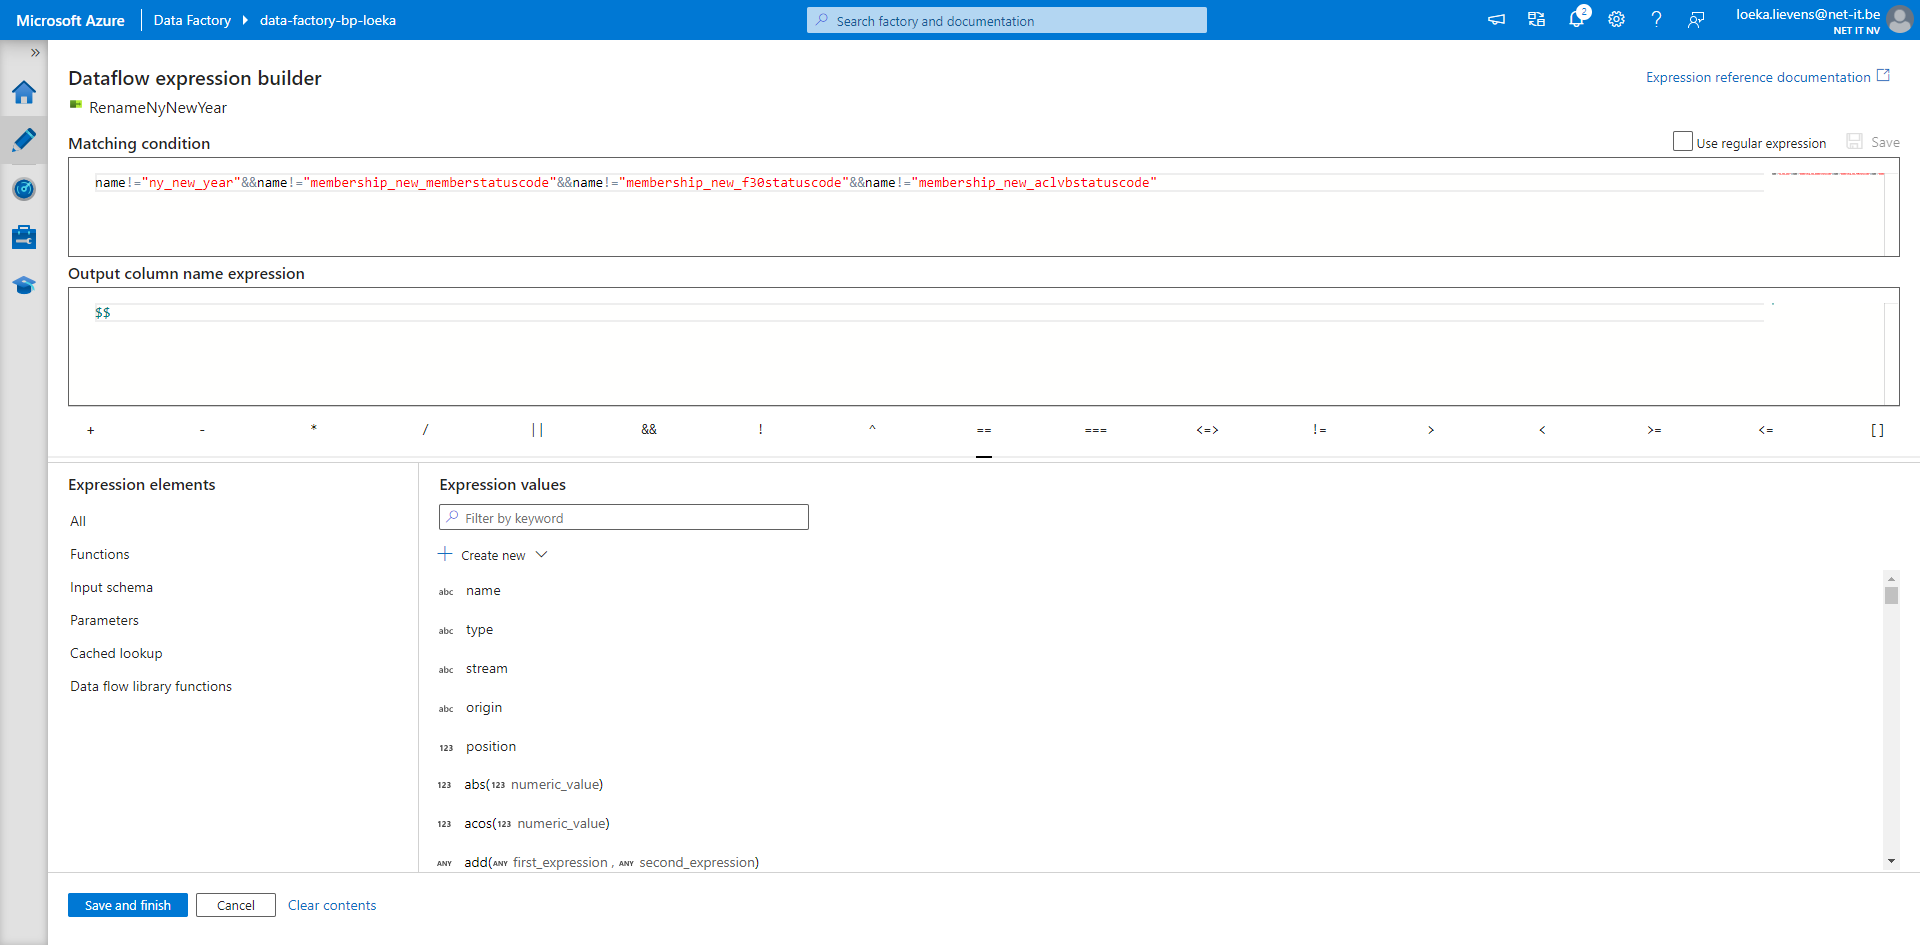
\includegraphics[width=1\textwidth]{./graphics/adf/new_membership_secondselect_2.png}
%\end{center}
%
%\texttt{De kolom `ny\_new\_year` wordt hernoemd naar `membership\_new\_year` en meerdere kolommon worden ongeselecteerd.}
%
%\begin{center}
%    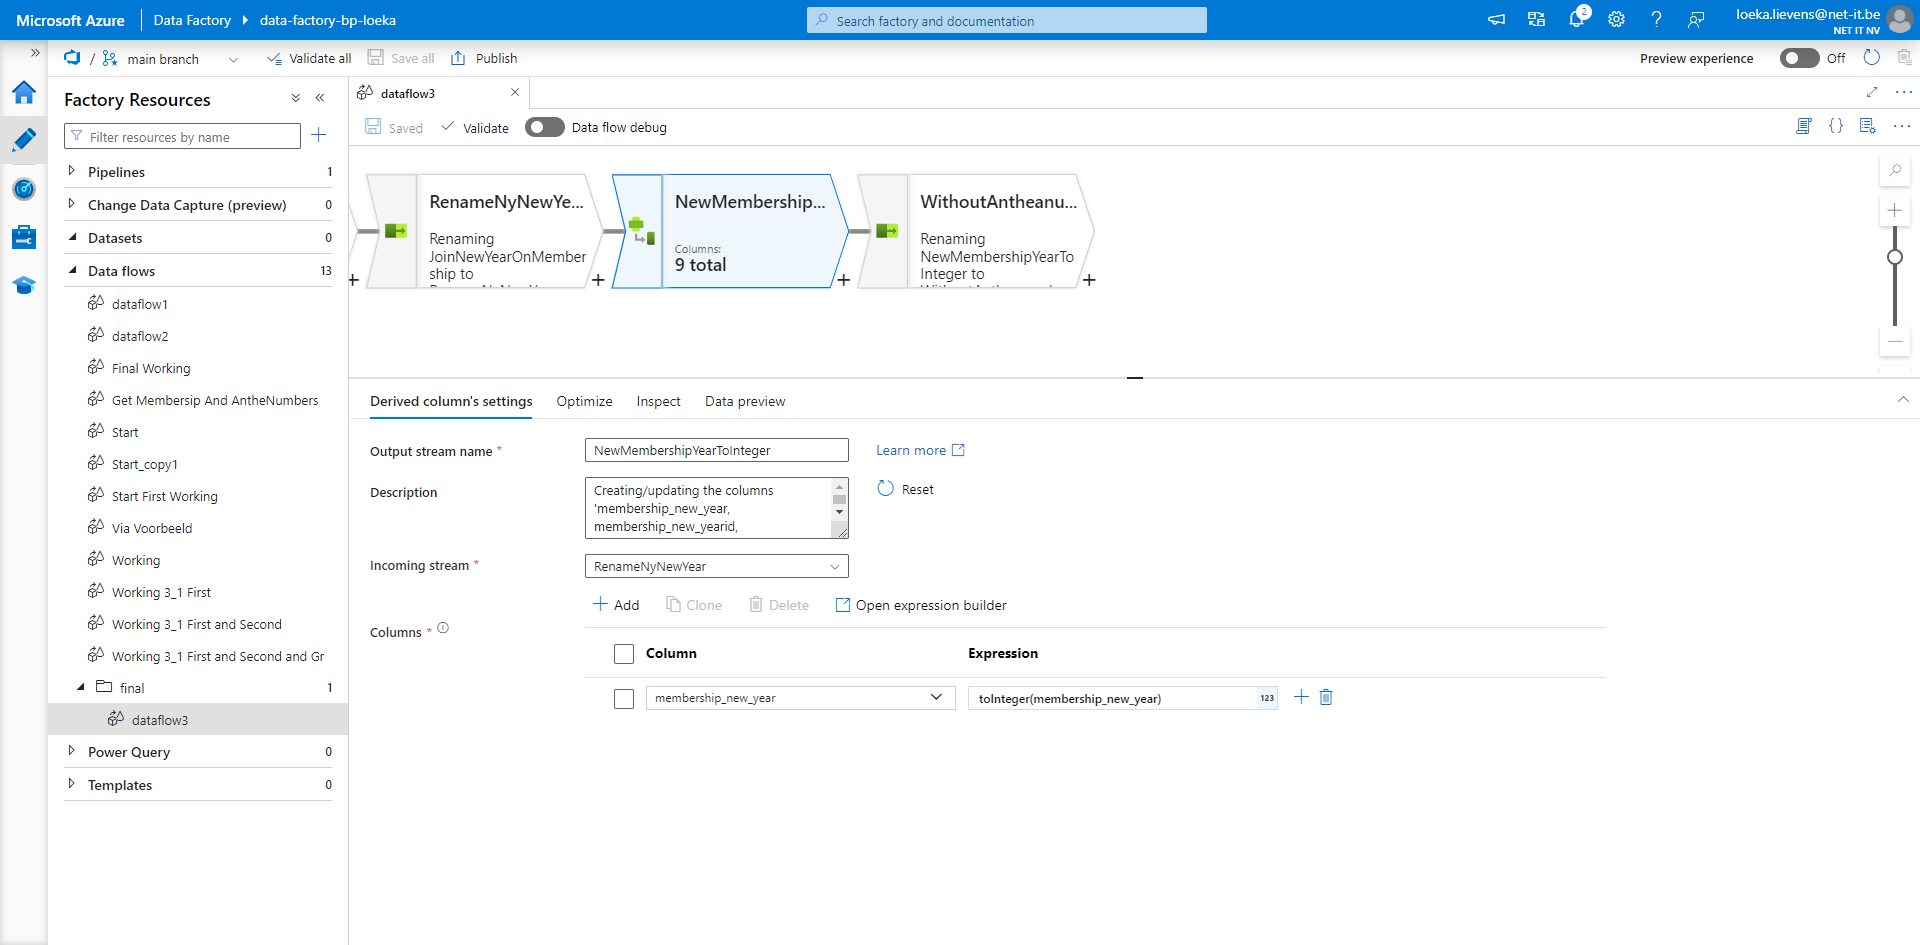
\includegraphics[width=1\textwidth]{./graphics/adf/new_membership_derive.png}
%\end{center}
%
%\texttt{`membership\_new\_year` wordt geparsed naar een integer.}
%
%\begin{center}
%    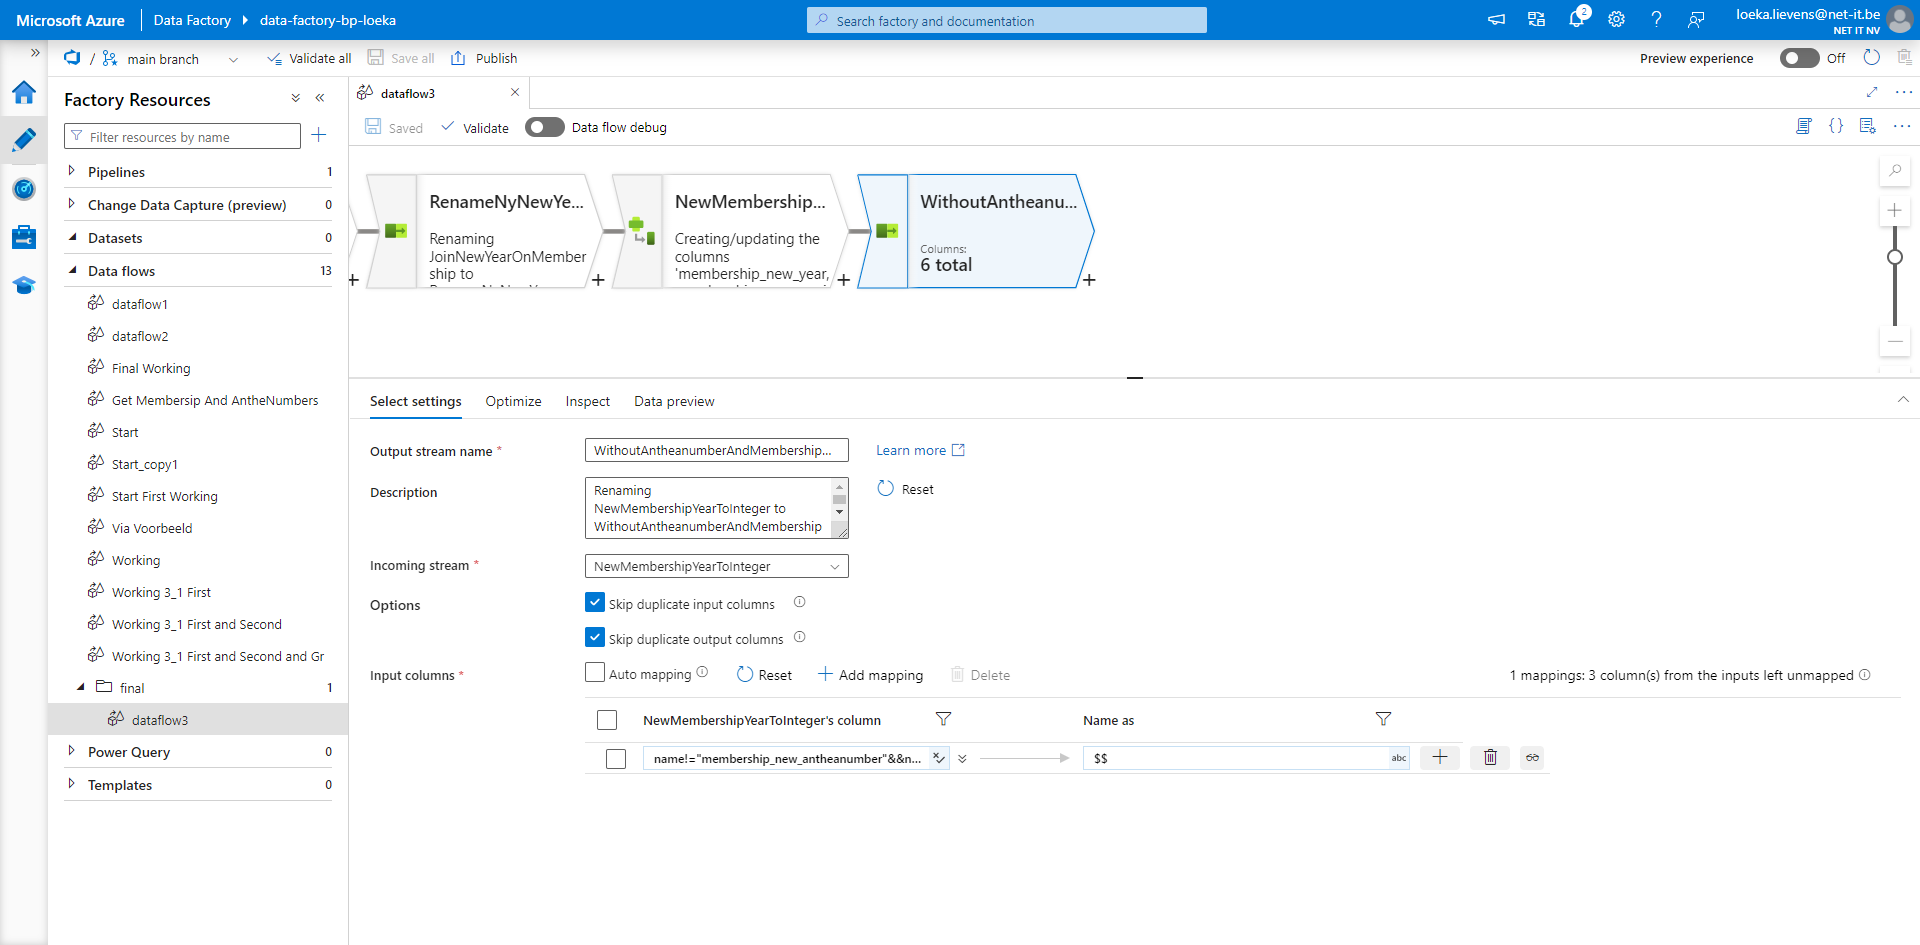
\includegraphics[width=1\textwidth]{./graphics/adf/new_membership_remove.png}
%\end{center}
%
%\begin{center}
%    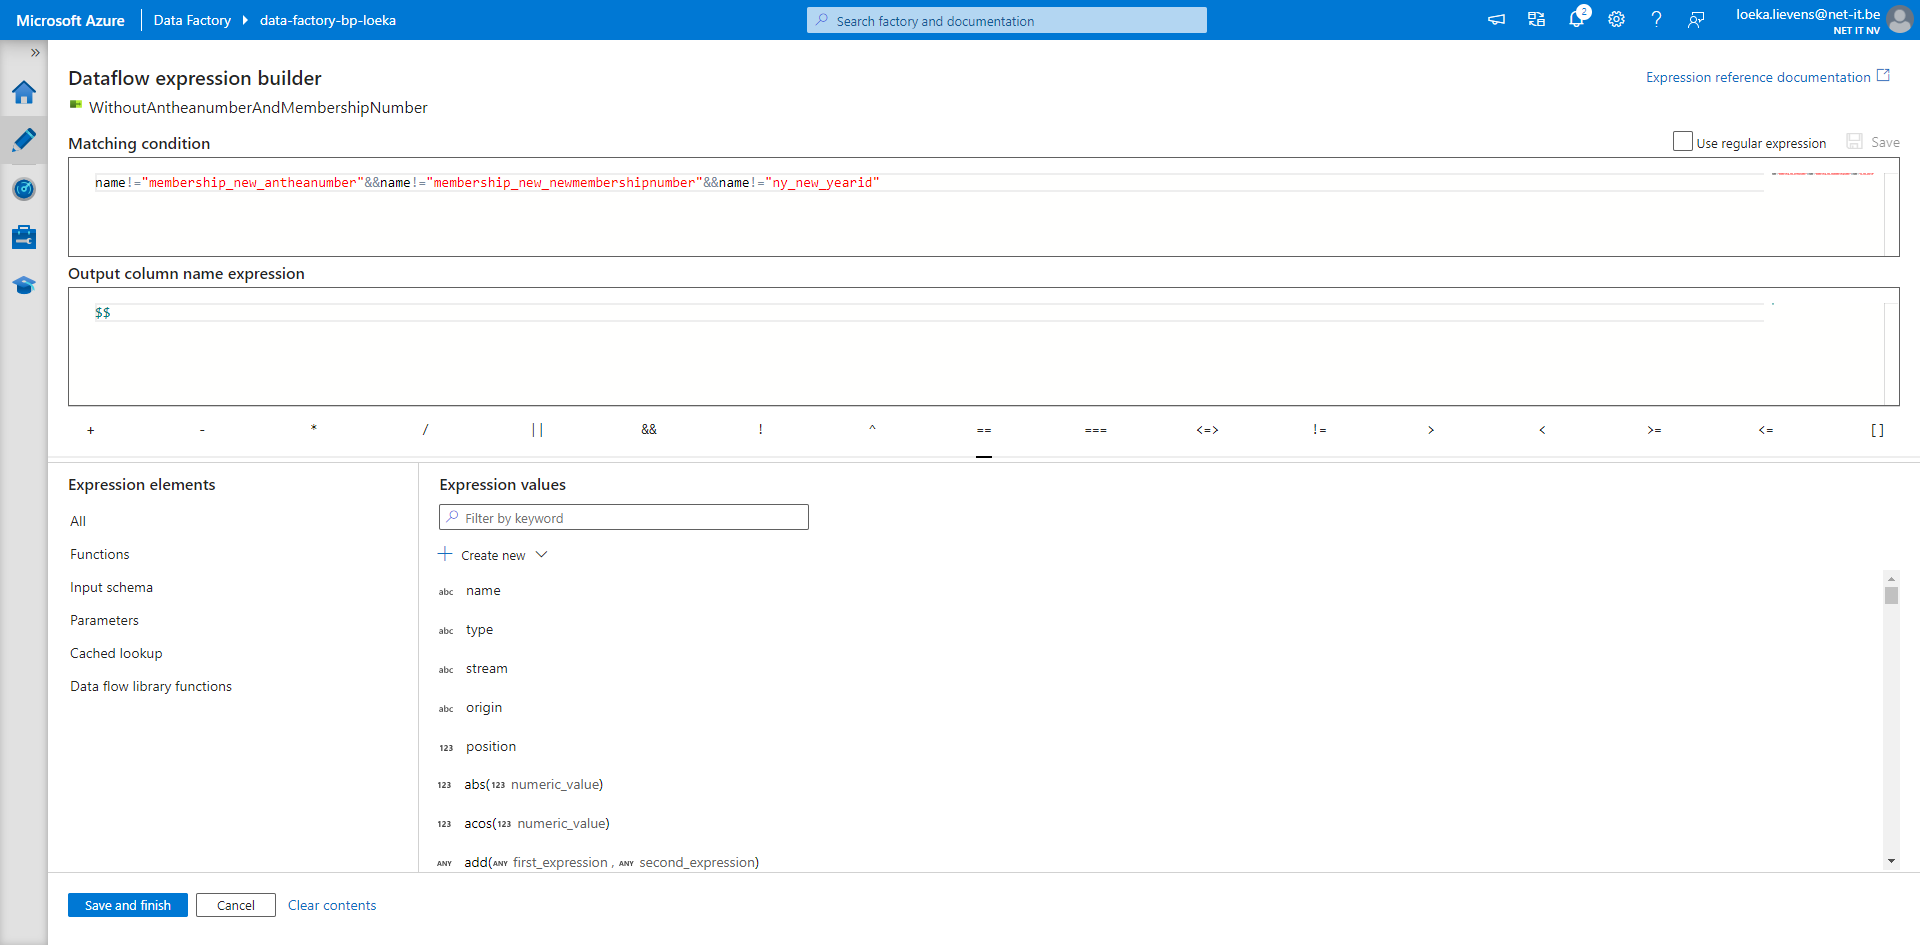
\includegraphics[width=1\textwidth]{./graphics/adf/new_membership_remove_2.png}
%\end{center}
%
%Meerdere kolommen worden ongeselecteerd.
%
%\paragraph{\texttt{Tabel new\_syndicalpremiumrequest}}
%
%\begin{center}
%    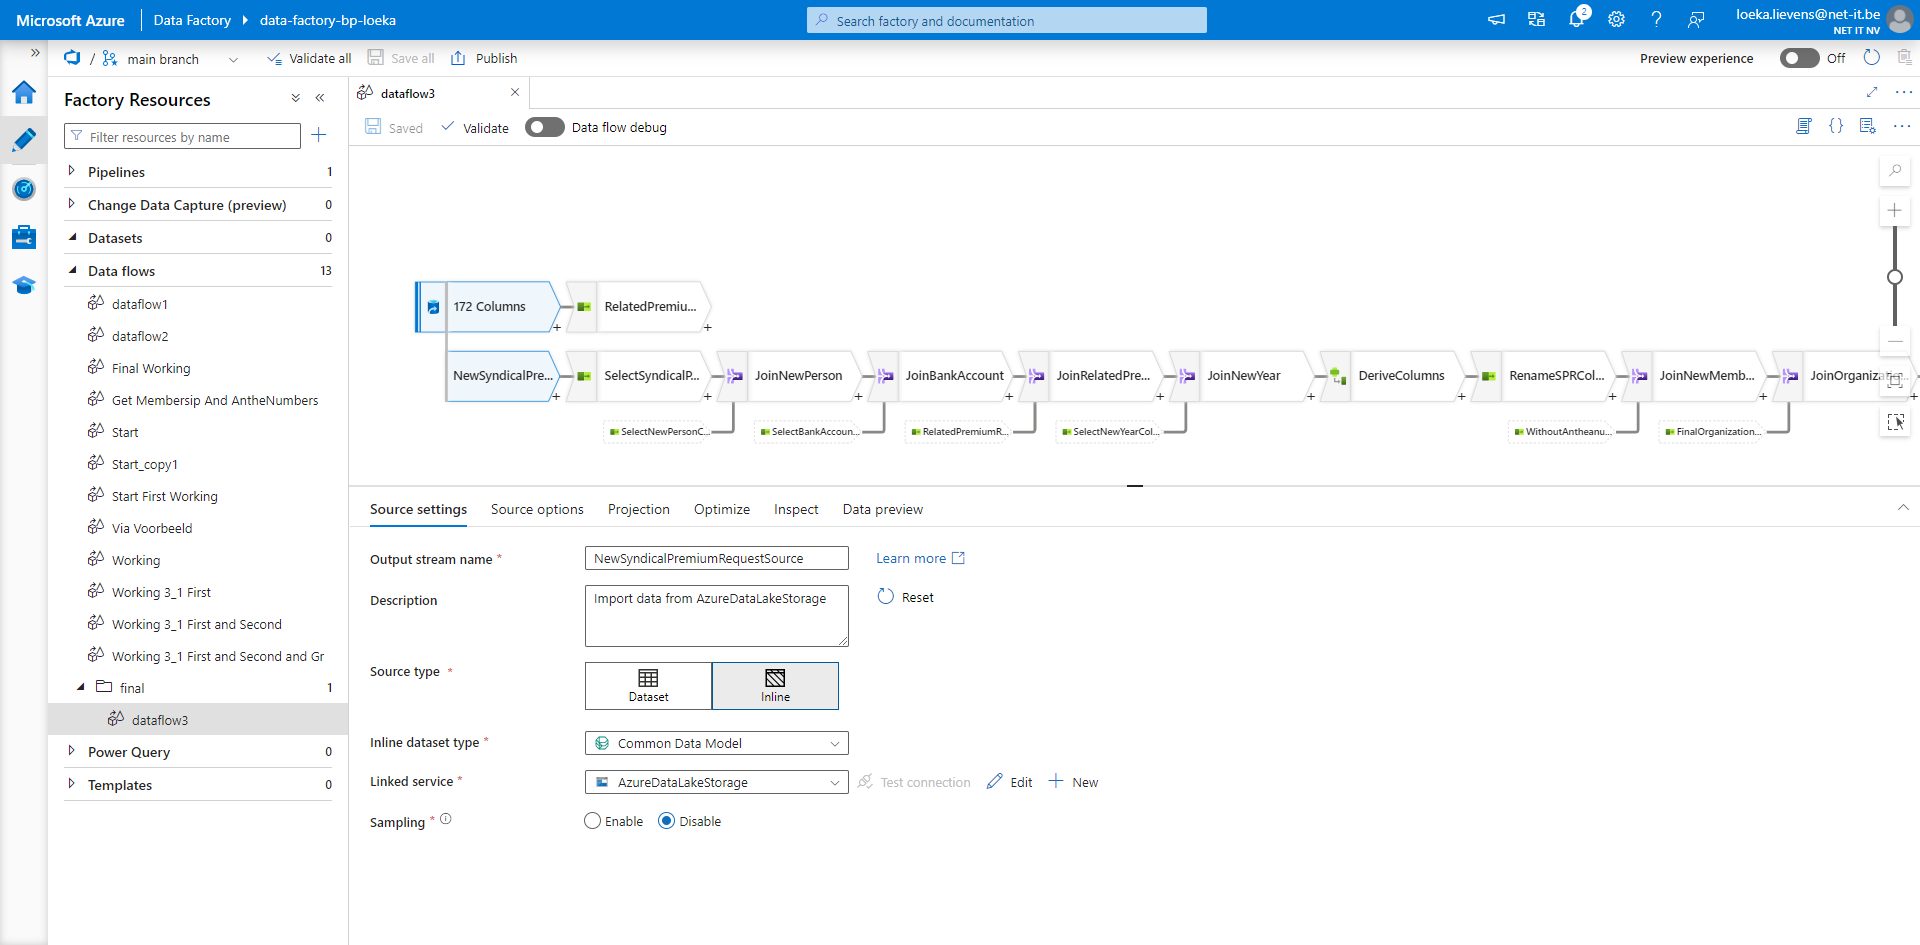
\includegraphics[width=1\textwidth]{./graphics/adf/spr_source.png}
%\end{center}
%
%\texttt{Er wordt een source toegevoegd voor de tabel new\_syndicalpremiumrequest. Na deze source is er een split, bij het bovenste gaan de kolommen voor de related syndical premium requests geselecteerd worden. Deze zijn belangrijk aangezien dit later gejoind wordt op syndical premium requests.}
%
%\begin{center}
%    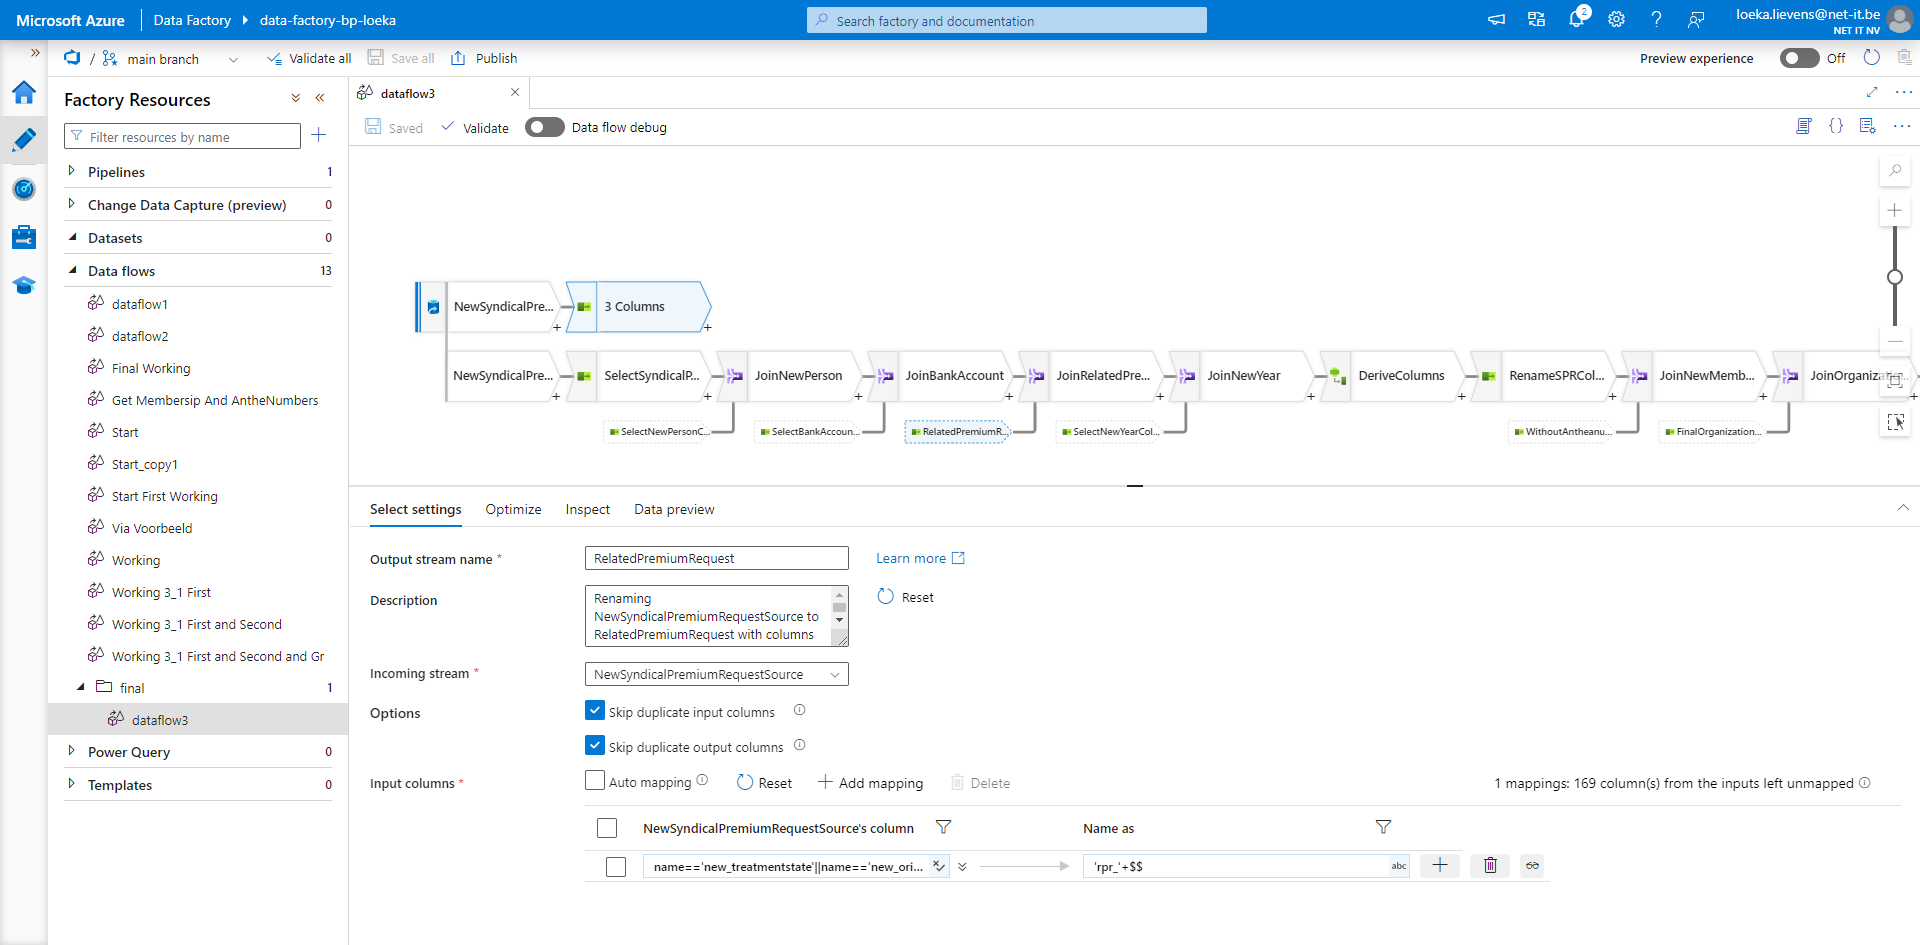
\includegraphics[width=1\textwidth]{./graphics/adf/spr_rpr_1.png}
%\end{center}
%
%\begin{center}
%    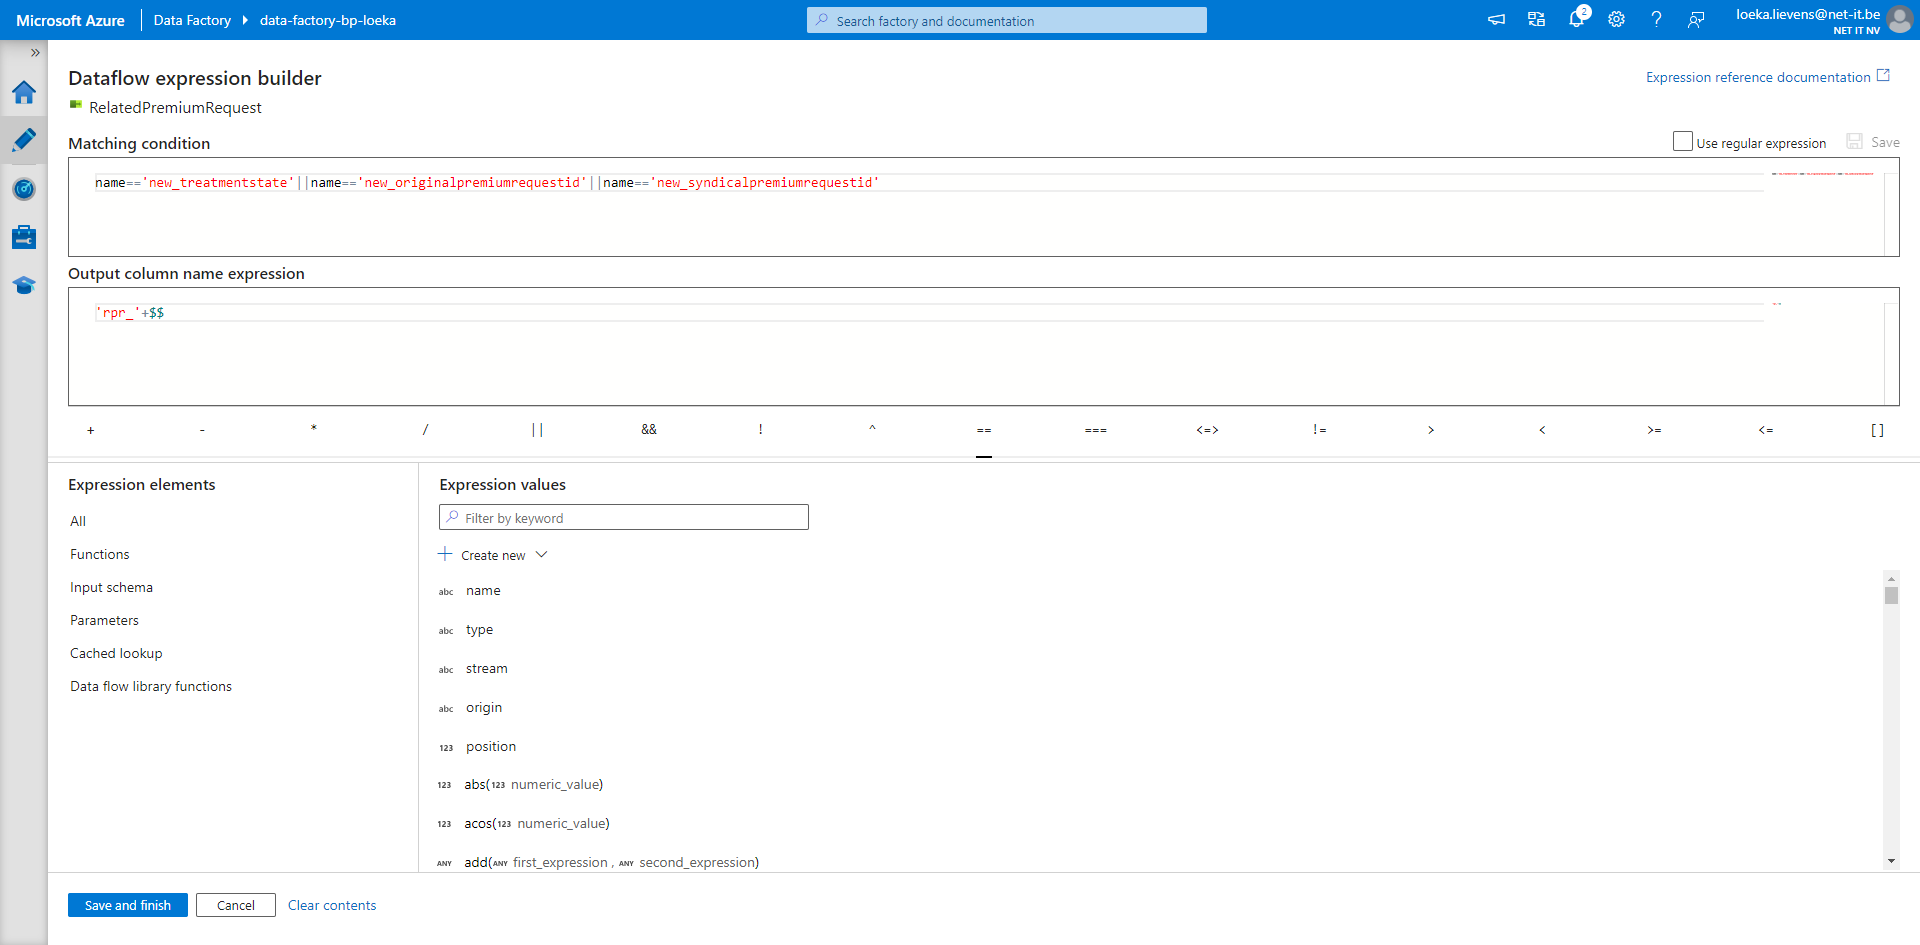
\includegraphics[width=1\textwidth]{./graphics/adf/spr_rpr_2.png}
%\end{center}
%
%\texttt{De nodige kolommen voor de related syndical premium requests worden geselecteerd en hernoemt met de prefix `rpr\_`.}
%
%\begin{center}
%    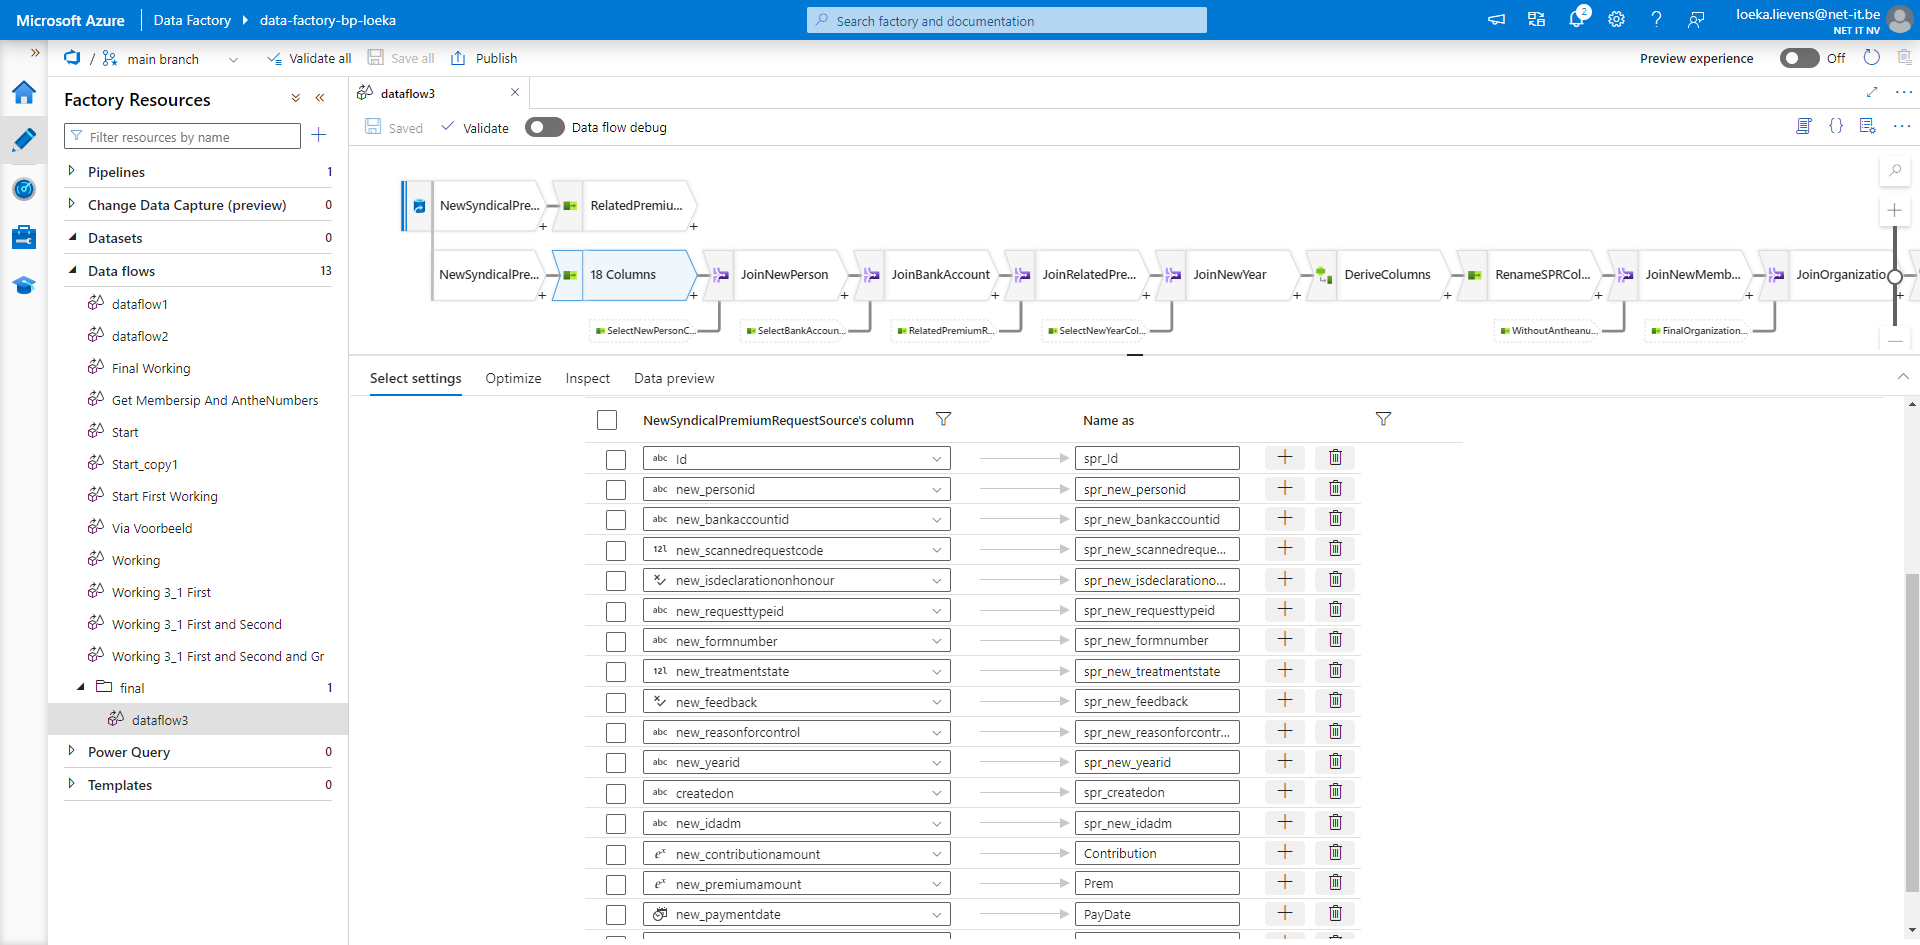
\includegraphics[width=1\textwidth]{./graphics/adf/spr_select.png}
%\end{center}
%
%\texttt{De nodige kolommen die gebruikt worden verder in de pipeline worden geselecteerd en hernoemt met de prefix `spr\_`. Ook zijn er kolommen zonder deze prefix, deze zullen later in het export bestand terecht komen.}
%
%\begin{center}
%    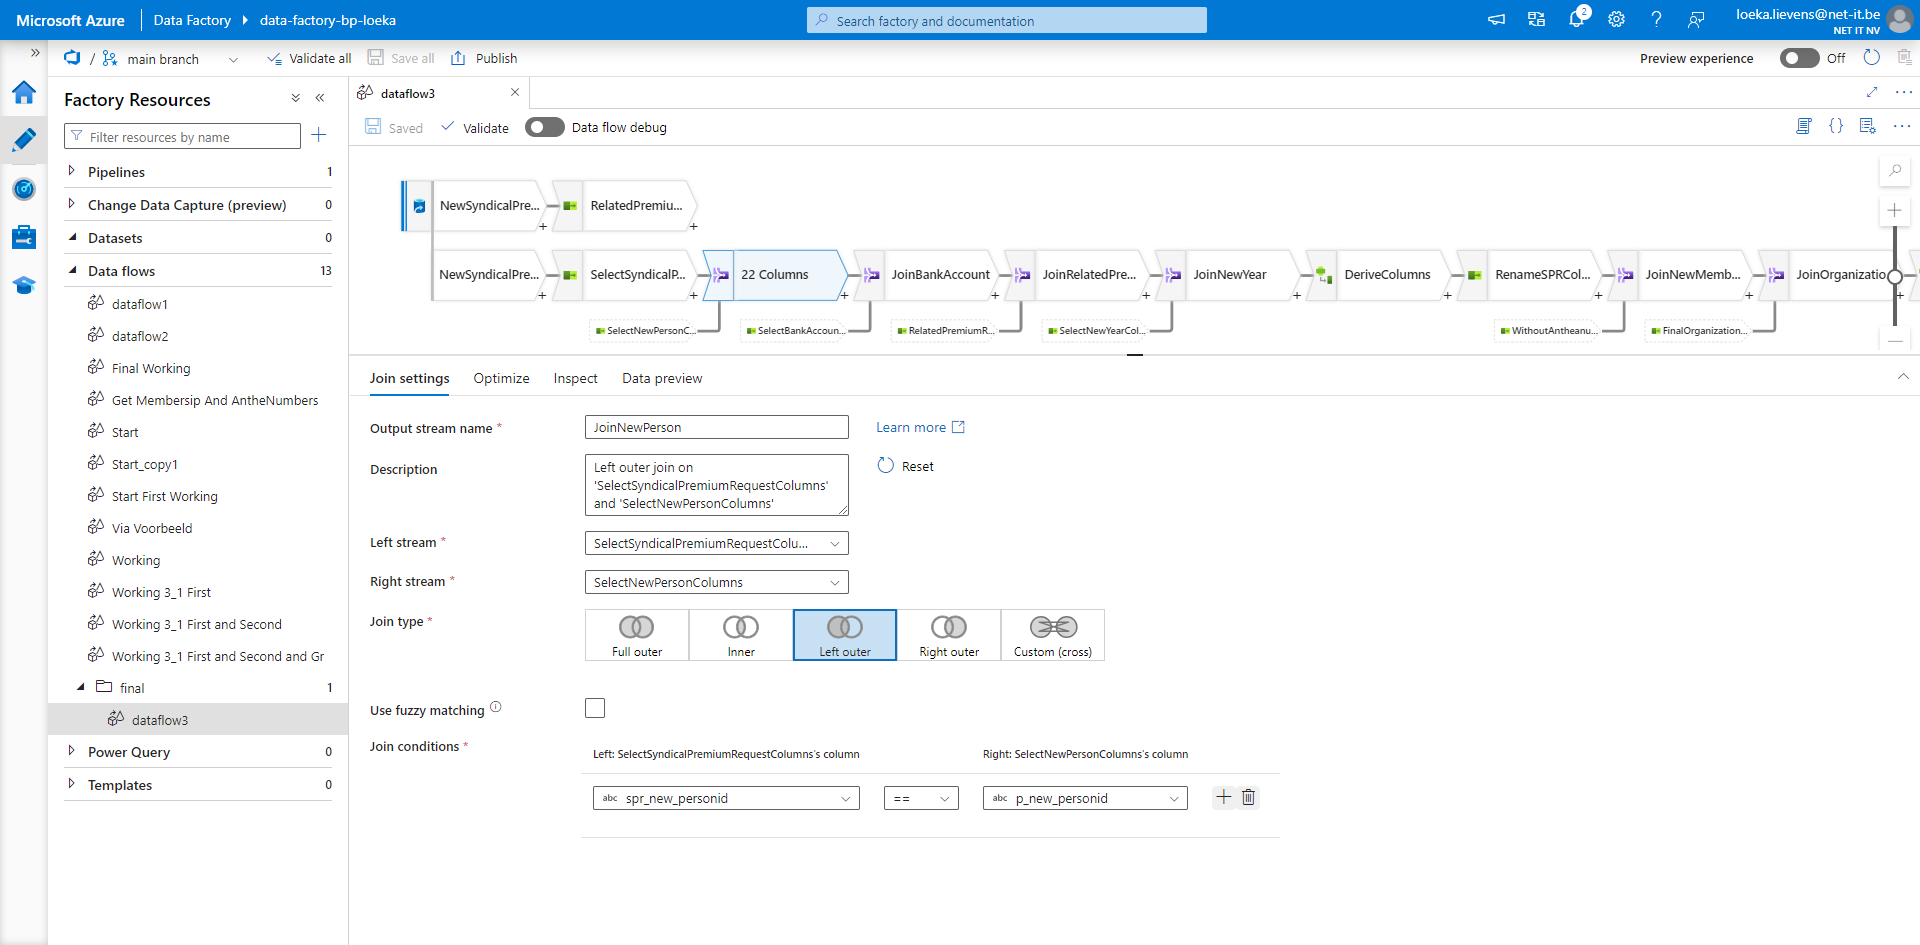
\includegraphics[width=1\textwidth]{./graphics/adf/spr_join_person.png}
%\end{center}
%
%\texttt{De tabel new\_person wordt gejoind aan de hand van id.}
%
%\begin{center}
%    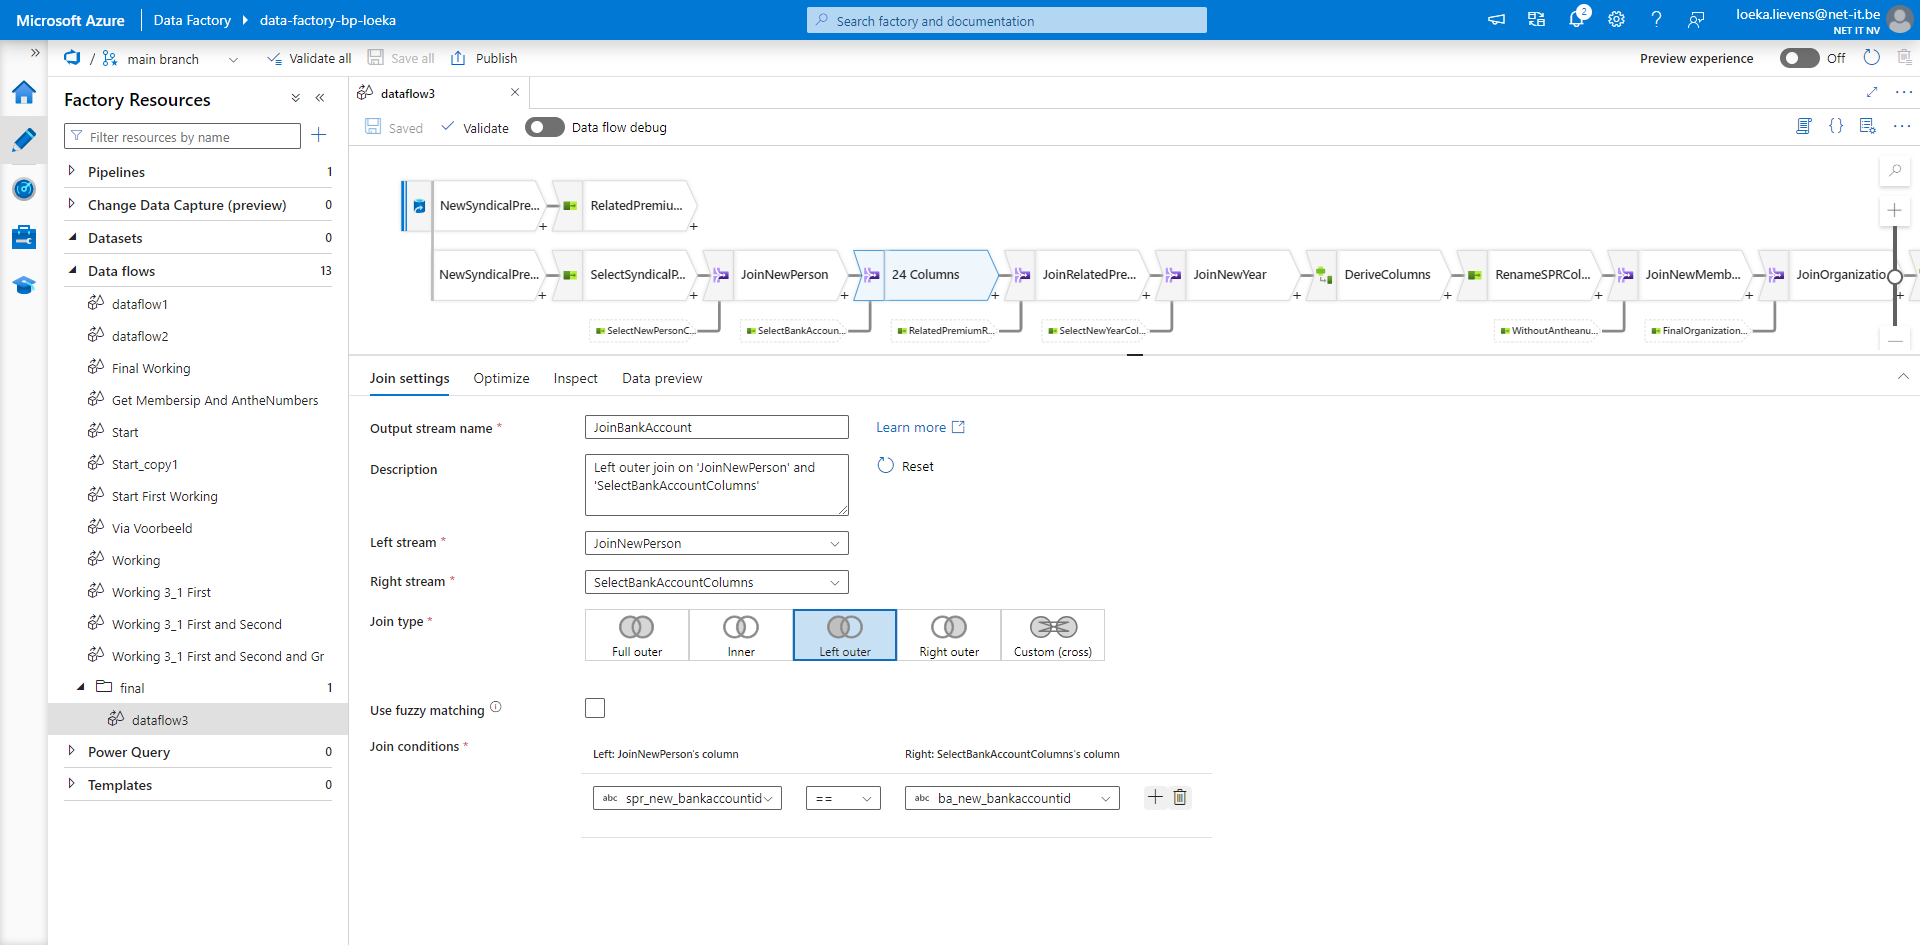
\includegraphics[width=1\textwidth]{./graphics/adf/spr_join_bankaccount.png}
%\end{center}
%
%\texttt{De tabel new\_bankaccount wordt gejoind aan de hand van id.}
%
%\begin{center}
%    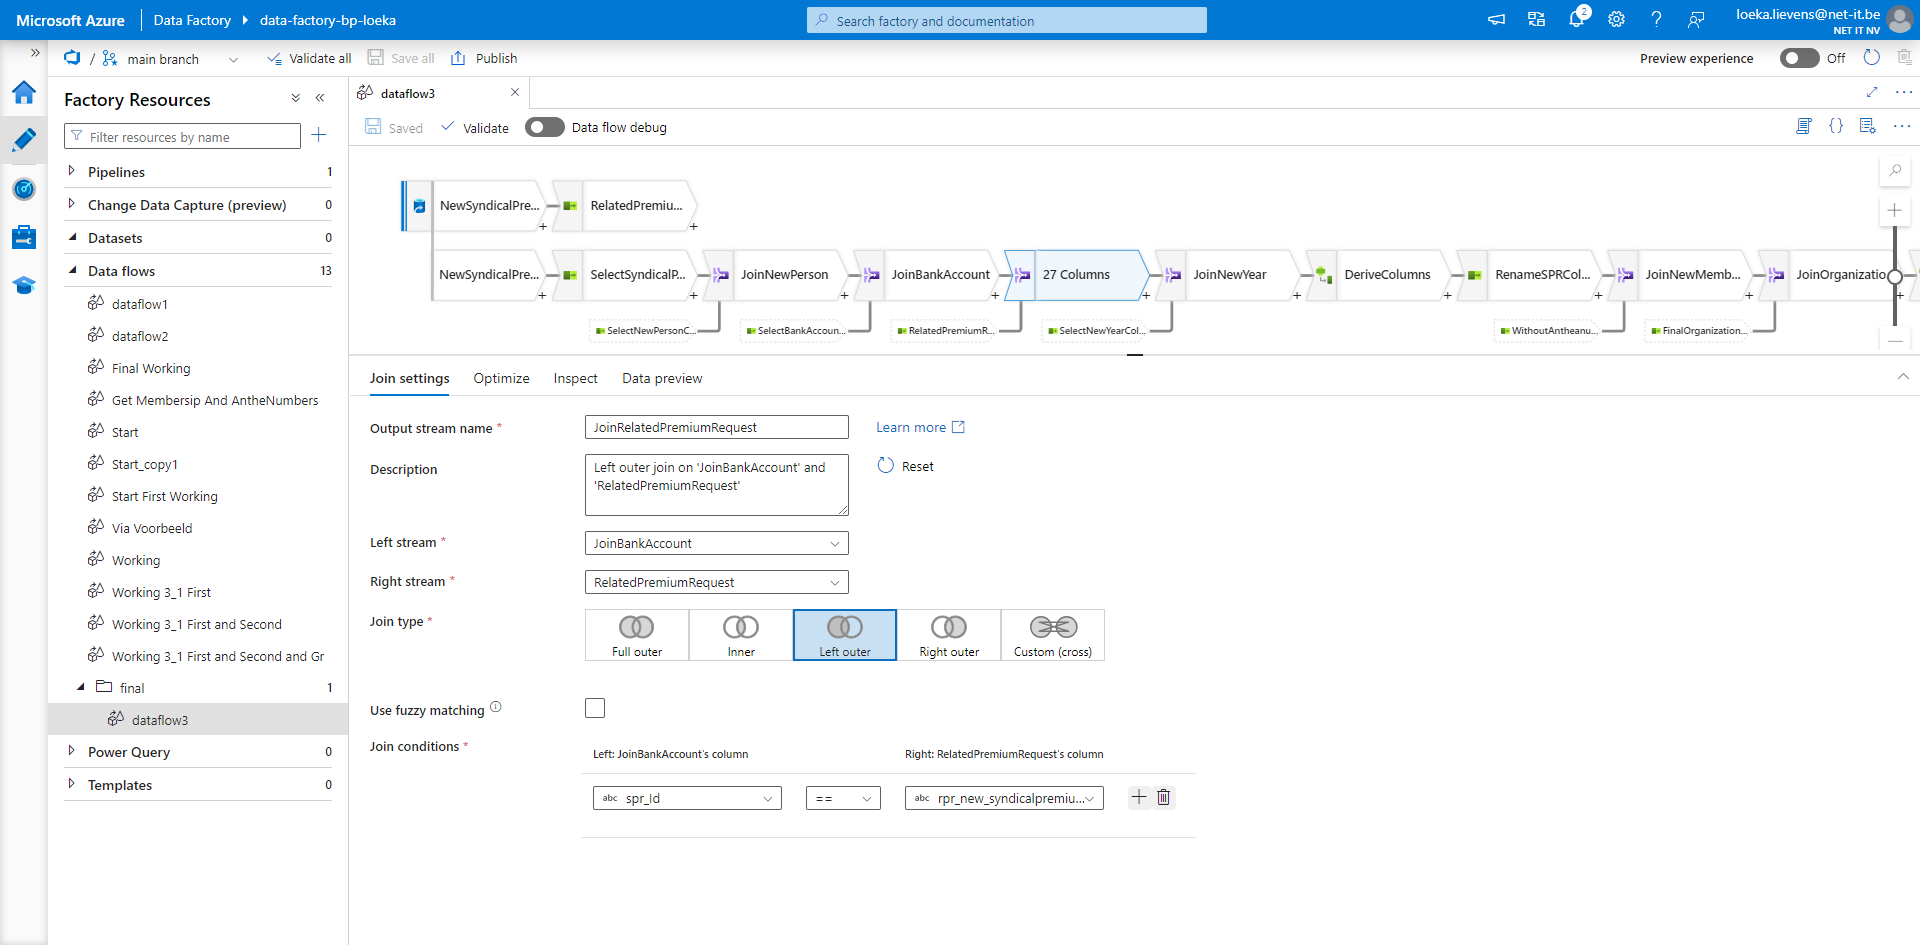
\includegraphics[width=1\textwidth]{./graphics/adf/spr_join_rpr.png}
%\end{center}
%
%\texttt{De related premium requests worden gejoind aan de hand van id.}
%
%\begin{center}
%    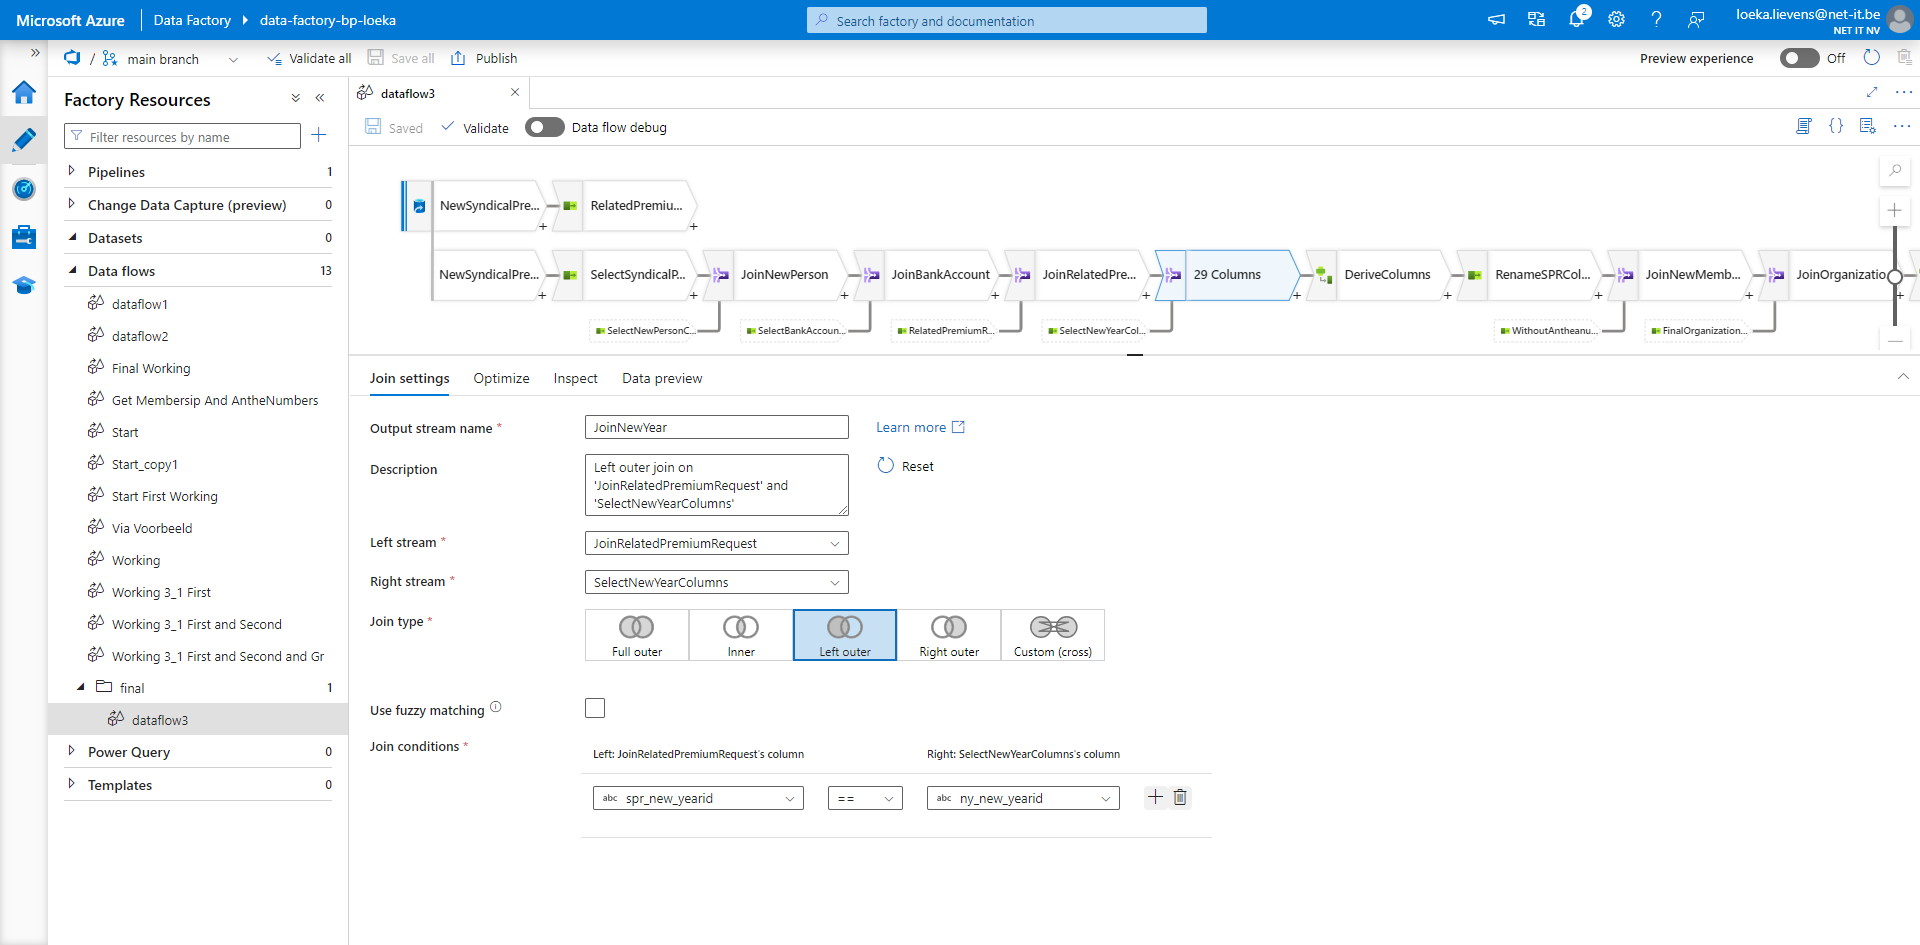
\includegraphics[width=1\textwidth]{./graphics/adf/spr_join_year.png}
%\end{center}
%
%\texttt{De tabel new\_year wordt gejoind aan de hand van id.}
%
%\begin{center}
%    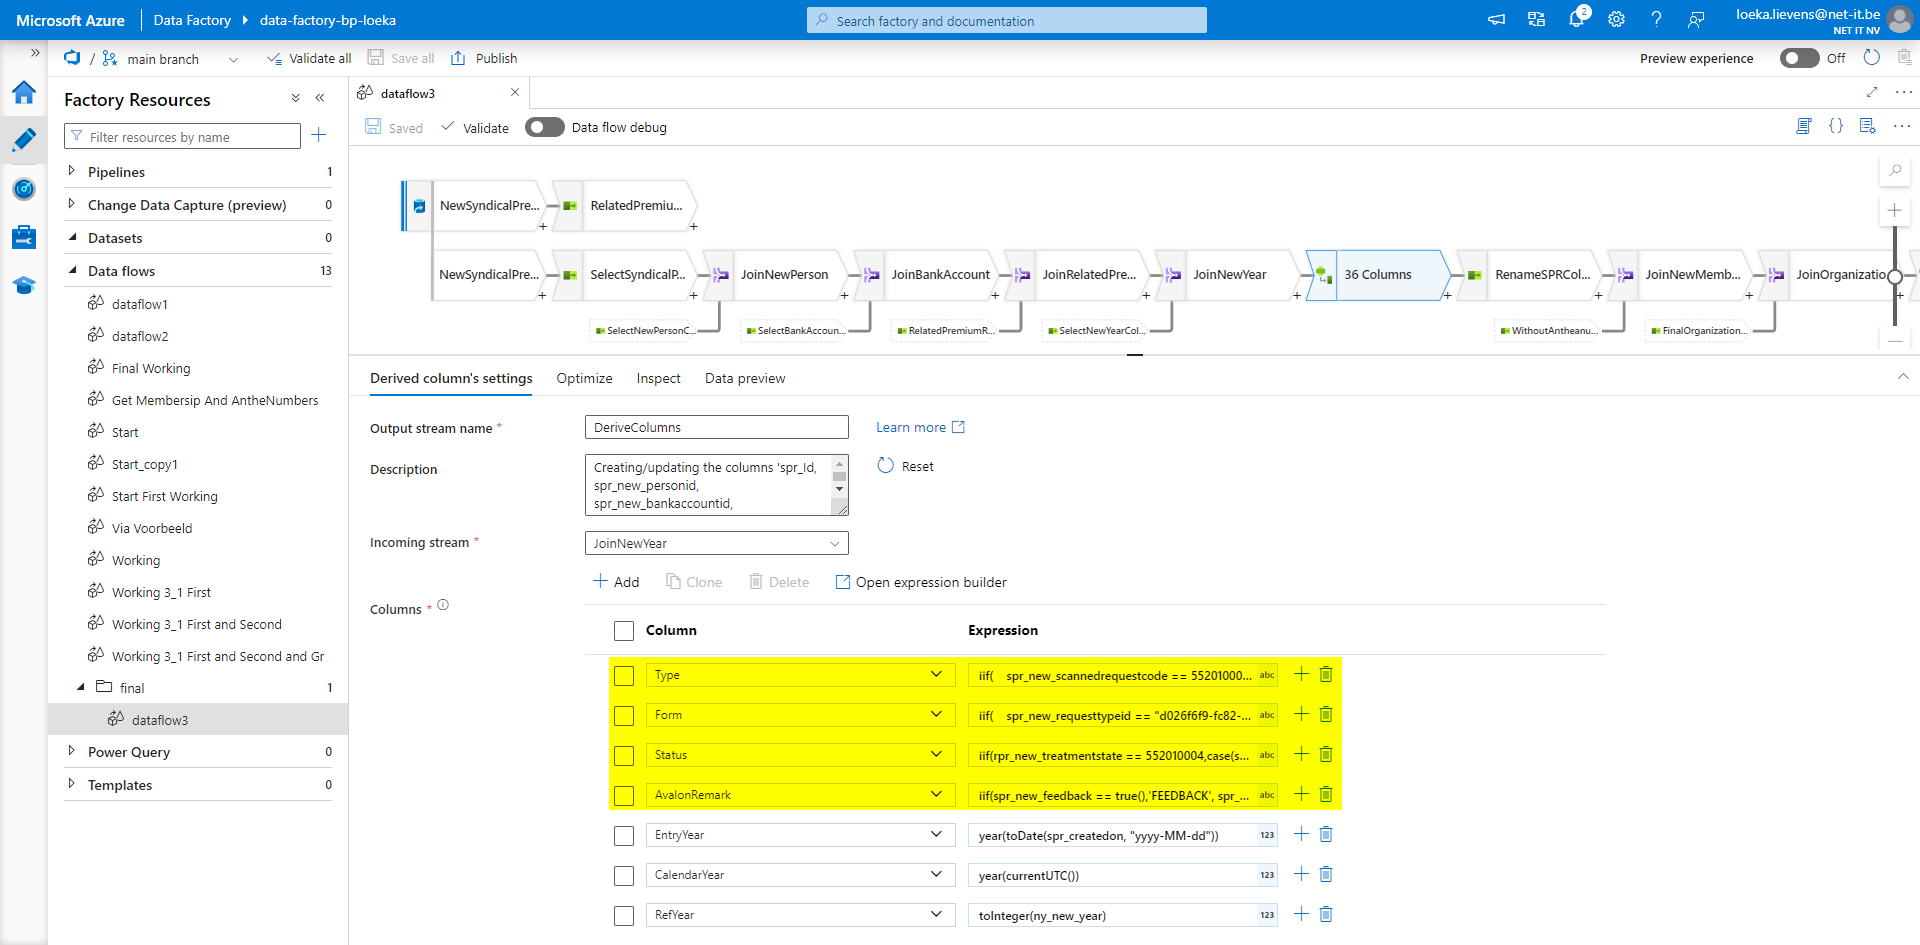
\includegraphics[width=1\textwidth]{./graphics/adf/spr_derive_1.png}
%\end{center}
%
%Er worden kolommen berekend die later in het export bestand zullen terecht komen.
%
%\begin{center}
%    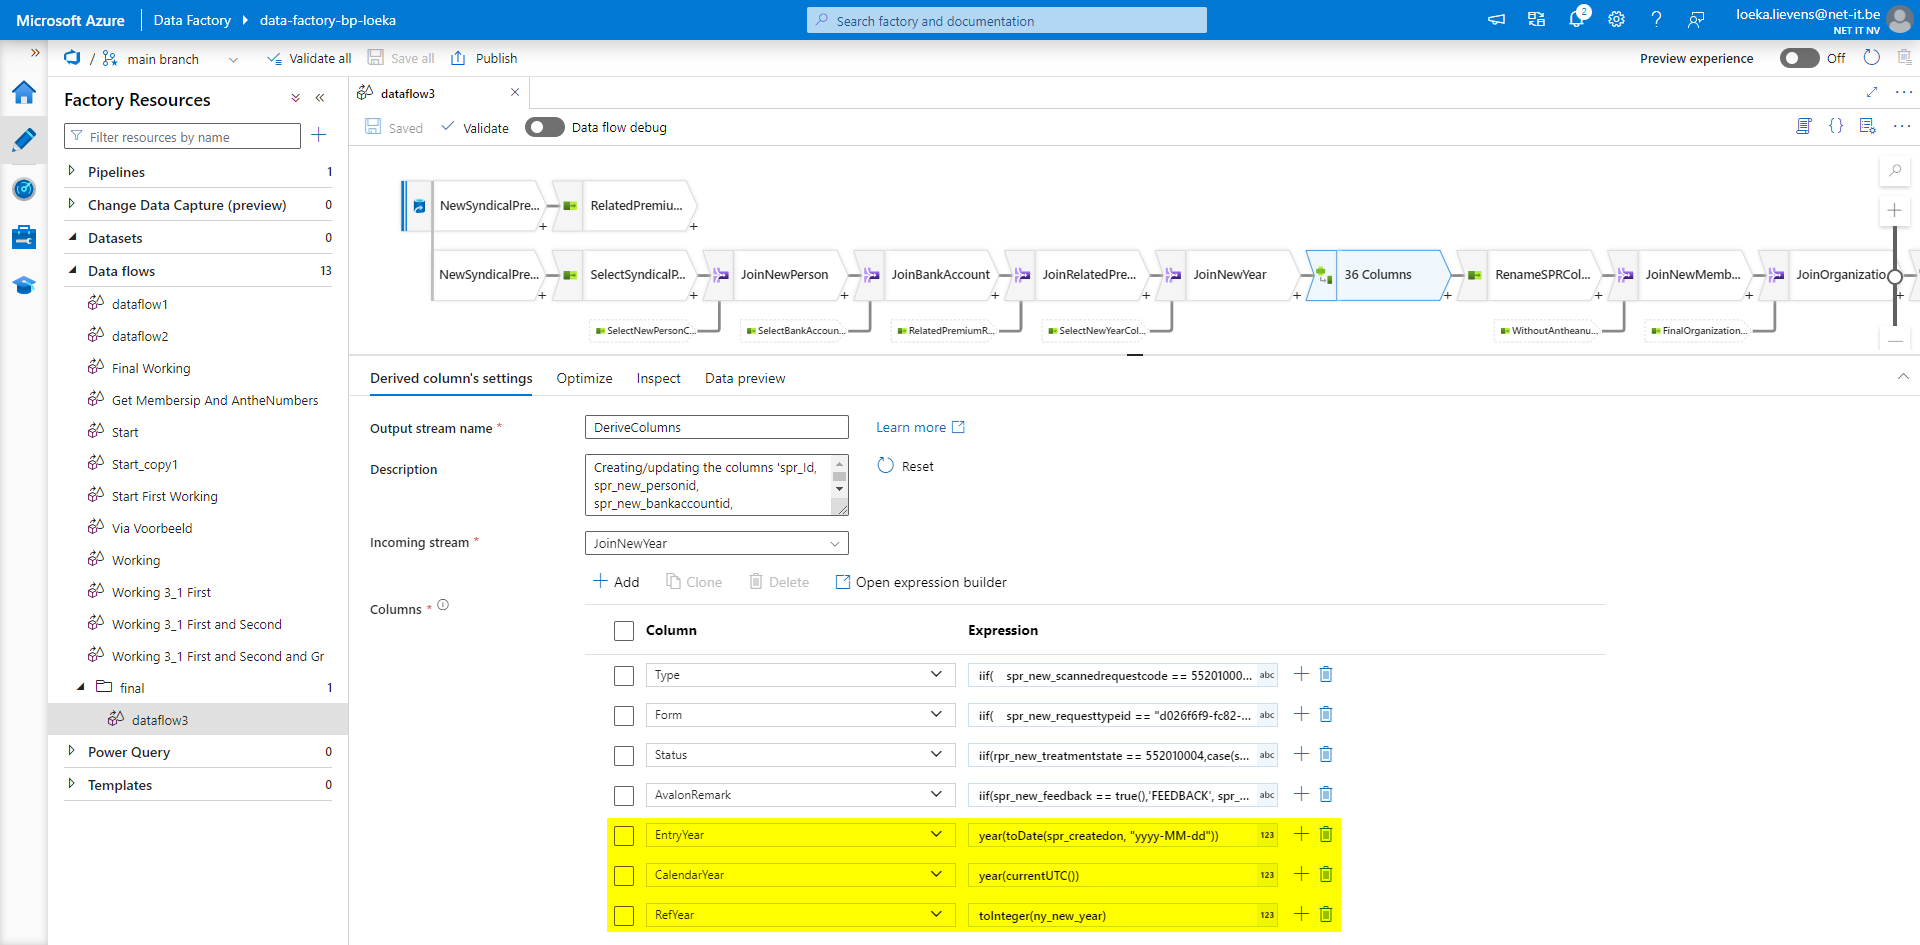
\includegraphics[width=1\textwidth]{./graphics/adf/spr_derive_2.png}
%\end{center}
%
%\texttt{De kolommen `EntryYear`, `CalendarYear` en `RefYear` zijn belangrijk. Met behulp van deze kolommen wordt er gekeken naar welke groepen een bepaalde premie (new\_syndicalpremiumrequest) zal gestuurd moeten worden.}
%
%\begin{center}
%    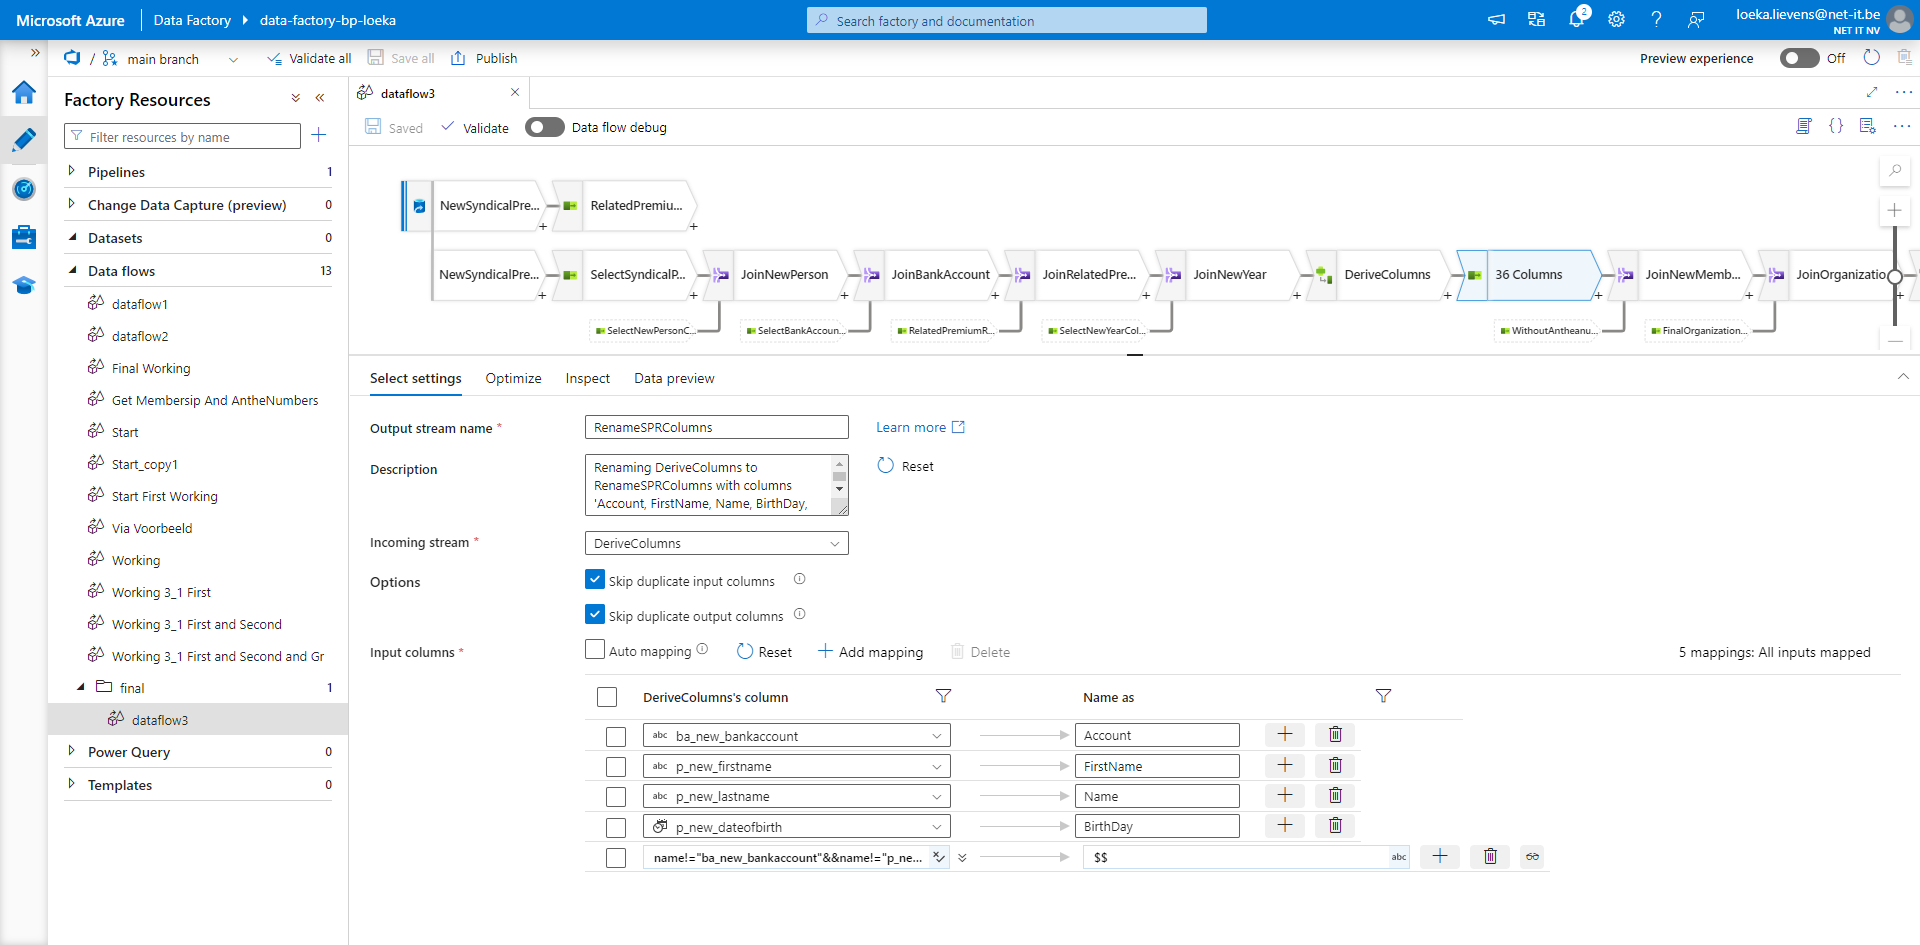
\includegraphics[width=1\textwidth]{./graphics/adf/spr_rename_1.png}
%\end{center}
%
%\begin{center}
%    \includegraphics[width=1\textwidth]{./graphics/adf/spr_rename_2.png}
%\end{center}
%
%Ook nu worden er kolommen hernoemd die in het export bestand zullen terecht komen. Daarnaast zijn er ook kolommen die ongeselecteerd worden doordat we deze verder in de pipeline niet meer nodig hebben.